\PassOptionsToPackage{unicode=true}{hyperref} % options for packages loaded elsewhere
\PassOptionsToPackage{hyphens}{url}
%
\documentclass[]{book}
\usepackage{lmodern}
\usepackage{amssymb,amsmath}
\usepackage{ifxetex,ifluatex}
\usepackage{fixltx2e} % provides \textsubscript
\ifnum 0\ifxetex 1\fi\ifluatex 1\fi=0 % if pdftex
  \usepackage[T1]{fontenc}
  \usepackage[utf8]{inputenc}
  \usepackage{textcomp} % provides euro and other symbols
\else % if luatex or xelatex
  \usepackage{unicode-math}
  \defaultfontfeatures{Ligatures=TeX,Scale=MatchLowercase}
\fi
% use upquote if available, for straight quotes in verbatim environments
\IfFileExists{upquote.sty}{\usepackage{upquote}}{}
% use microtype if available
\IfFileExists{microtype.sty}{%
\usepackage[]{microtype}
\UseMicrotypeSet[protrusion]{basicmath} % disable protrusion for tt fonts
}{}
\IfFileExists{parskip.sty}{%
\usepackage{parskip}
}{% else
\setlength{\parindent}{0pt}
\setlength{\parskip}{6pt plus 2pt minus 1pt}
}
\usepackage{hyperref}
\hypersetup{
            pdftitle={dads manual},
            pdfauthor={Thomas Guillerme (guillert@tcd.ie), Alex Slavenko (email) and others},
            pdfborder={0 0 0},
            breaklinks=true}
\urlstyle{same}  % don't use monospace font for urls
\usepackage{color}
\usepackage{fancyvrb}
\newcommand{\VerbBar}{|}
\newcommand{\VERB}{\Verb[commandchars=\\\{\}]}
\DefineVerbatimEnvironment{Highlighting}{Verbatim}{commandchars=\\\{\}}
% Add ',fontsize=\small' for more characters per line
\usepackage{framed}
\definecolor{shadecolor}{RGB}{248,248,248}
\newenvironment{Shaded}{\begin{snugshade}}{\end{snugshade}}
\newcommand{\AlertTok}[1]{\textcolor[rgb]{0.94,0.16,0.16}{#1}}
\newcommand{\AnnotationTok}[1]{\textcolor[rgb]{0.56,0.35,0.01}{\textbf{\textit{#1}}}}
\newcommand{\AttributeTok}[1]{\textcolor[rgb]{0.77,0.63,0.00}{#1}}
\newcommand{\BaseNTok}[1]{\textcolor[rgb]{0.00,0.00,0.81}{#1}}
\newcommand{\BuiltInTok}[1]{#1}
\newcommand{\CharTok}[1]{\textcolor[rgb]{0.31,0.60,0.02}{#1}}
\newcommand{\CommentTok}[1]{\textcolor[rgb]{0.56,0.35,0.01}{\textit{#1}}}
\newcommand{\CommentVarTok}[1]{\textcolor[rgb]{0.56,0.35,0.01}{\textbf{\textit{#1}}}}
\newcommand{\ConstantTok}[1]{\textcolor[rgb]{0.00,0.00,0.00}{#1}}
\newcommand{\ControlFlowTok}[1]{\textcolor[rgb]{0.13,0.29,0.53}{\textbf{#1}}}
\newcommand{\DataTypeTok}[1]{\textcolor[rgb]{0.13,0.29,0.53}{#1}}
\newcommand{\DecValTok}[1]{\textcolor[rgb]{0.00,0.00,0.81}{#1}}
\newcommand{\DocumentationTok}[1]{\textcolor[rgb]{0.56,0.35,0.01}{\textbf{\textit{#1}}}}
\newcommand{\ErrorTok}[1]{\textcolor[rgb]{0.64,0.00,0.00}{\textbf{#1}}}
\newcommand{\ExtensionTok}[1]{#1}
\newcommand{\FloatTok}[1]{\textcolor[rgb]{0.00,0.00,0.81}{#1}}
\newcommand{\FunctionTok}[1]{\textcolor[rgb]{0.00,0.00,0.00}{#1}}
\newcommand{\ImportTok}[1]{#1}
\newcommand{\InformationTok}[1]{\textcolor[rgb]{0.56,0.35,0.01}{\textbf{\textit{#1}}}}
\newcommand{\KeywordTok}[1]{\textcolor[rgb]{0.13,0.29,0.53}{\textbf{#1}}}
\newcommand{\NormalTok}[1]{#1}
\newcommand{\OperatorTok}[1]{\textcolor[rgb]{0.81,0.36,0.00}{\textbf{#1}}}
\newcommand{\OtherTok}[1]{\textcolor[rgb]{0.56,0.35,0.01}{#1}}
\newcommand{\PreprocessorTok}[1]{\textcolor[rgb]{0.56,0.35,0.01}{\textit{#1}}}
\newcommand{\RegionMarkerTok}[1]{#1}
\newcommand{\SpecialCharTok}[1]{\textcolor[rgb]{0.00,0.00,0.00}{#1}}
\newcommand{\SpecialStringTok}[1]{\textcolor[rgb]{0.31,0.60,0.02}{#1}}
\newcommand{\StringTok}[1]{\textcolor[rgb]{0.31,0.60,0.02}{#1}}
\newcommand{\VariableTok}[1]{\textcolor[rgb]{0.00,0.00,0.00}{#1}}
\newcommand{\VerbatimStringTok}[1]{\textcolor[rgb]{0.31,0.60,0.02}{#1}}
\newcommand{\WarningTok}[1]{\textcolor[rgb]{0.56,0.35,0.01}{\textbf{\textit{#1}}}}
\usepackage{longtable,booktabs}
% Fix footnotes in tables (requires footnote package)
\IfFileExists{footnote.sty}{\usepackage{footnote}\makesavenoteenv{longtable}}{}
\usepackage{graphicx,grffile}
\makeatletter
\def\maxwidth{\ifdim\Gin@nat@width>\linewidth\linewidth\else\Gin@nat@width\fi}
\def\maxheight{\ifdim\Gin@nat@height>\textheight\textheight\else\Gin@nat@height\fi}
\makeatother
% Scale images if necessary, so that they will not overflow the page
% margins by default, and it is still possible to overwrite the defaults
% using explicit options in \includegraphics[width, height, ...]{}
\setkeys{Gin}{width=\maxwidth,height=\maxheight,keepaspectratio}
\setlength{\emergencystretch}{3em}  % prevent overfull lines
\providecommand{\tightlist}{%
  \setlength{\itemsep}{0pt}\setlength{\parskip}{0pt}}
\setcounter{secnumdepth}{5}
% Redefines (sub)paragraphs to behave more like sections
\ifx\paragraph\undefined\else
\let\oldparagraph\paragraph
\renewcommand{\paragraph}[1]{\oldparagraph{#1}\mbox{}}
\fi
\ifx\subparagraph\undefined\else
\let\oldsubparagraph\subparagraph
\renewcommand{\subparagraph}[1]{\oldsubparagraph{#1}\mbox{}}
\fi

% set default figure placement to htbp
\makeatletter
\def\fps@figure{htbp}
\makeatother

\usepackage{booktabs}
\usepackage[]{natbib}
\bibliographystyle{plainnat}

\title{dads manual}
\author{Thomas Guillerme (\href{mailto:guillert@tcd.ie}{\nolinkurl{guillert@tcd.ie}}), Alex Slavenko (email) and others}
\date{2021-01-12}

\begin{document}
\maketitle

{
\setcounter{tocdepth}{1}
\tableofcontents
}
\hypertarget{dads-disparity-and-diversity-simulations.}{%
\chapter{\texorpdfstring{\texttt{dads}: disparity and diversity simulations.}{dads: disparity and diversity simulations.}}\label{dads-disparity-and-diversity-simulations.}}

Allowing to simulate disparity and diversity at the same time with interaction between both.

The core of this package is based on the \href{https://github.com/cran/diversitree/blob/master/R/simulate-bd.R}{\texttt{diversitree} birth-death algorithm}.

\hypertarget{what-is-dads}{%
\section{\texorpdfstring{What is \texttt{dads}?}{What is dads?}}\label{what-is-dads}}

There are some very good packages out there to simulate birth death trees (like \href{https://github.com/tanja819/TreeSim}{TreeSim}) or even packages simulating traits (disparity) and diversity jointly (like \href{https://github.com/cran/RPANDA}{RPANDA} or \href{https://github.com/PuttickMacroevolution/PETER}{PETER}).
We strongly advice you have a look at these packages first as they might be more appropriate for your tasks.

\texttt{dads} aims to be a highly modular and friendly version of all these packages: it allows to simulate disparity and diversity jointly with a vast array of options that can be easily modified by users.
For example, you can easily generate any type of process to generate a trait (BM, OU, something else, etc\ldots{}) in multiple dependent or independent dimensions through \texttt{"traits"} objects.
You can then specify how the traits should affect disparity through \texttt{"modifiers"} objects. And finally you can create events (like mass extinctions) through \texttt{"events"} objects.
These objects and how to modify them will be detailed throughout this manual.
Finally we are putting an emphasise in the development of this package on the speed and reliability of the functions.

\hypertarget{modular}{%
\subsection{Modular?}\label{modular}}

Because their is an infinite way you might want to generate disparity and diversity (different traits, different modifiers and different events), the \texttt{dads} package is designed to make all these parts easy to code separately and integrate them easily in the \texttt{dads} core functions.
This allows you to simulate finely tuned multidimensional data for your specific project!

\hypertarget{installing-and-running-the-package}{%
\section{Installing and running the package}\label{installing-and-running-the-package}}

You can install this package easily, directly from the github:

\begin{Shaded}
\begin{Highlighting}[]
\CommentTok{## Checking if devtools is already installed}
\ControlFlowTok{if}\NormalTok{(}\OperatorTok{!}\KeywordTok{require}\NormalTok{(devtools)) }\KeywordTok{install.packages}\NormalTok{(}\StringTok{"devtools"}\NormalTok{)}

\CommentTok{## Installing the latest version directly from GitHub}
\NormalTok{devtools}\OperatorTok{::}\KeywordTok{install_github}\NormalTok{(}\StringTok{"TGuillerme/dads"}\NormalTok{)}
\end{Highlighting}
\end{Shaded}

\hypertarget{help}{%
\section{Help}\label{help}}

If you need help with the package, hopefully the following manual will be useful.
However, parts of this package are still in development and some other parts are probably not covered.
Thus if you have suggestions or comments on on what has already been developed or will be developed, please send me an email (\href{mailto:guillert@tcd.ie}{\nolinkurl{guillert@tcd.ie}}) or if you are a GitHub user, directly create an issue on the \href{https://github.com/TGuillerme/dads}{GitHub page}.
Doing so will not only hopefully help you but also other users since it will help improve this manual!

\hypertarget{how-does-dads-work}{%
\section{\texorpdfstring{How does \texttt{dads} work?}{How does dads work?}}\label{how-does-dads-work}}

Basically, the \texttt{dads} function intakes your personalised \texttt{traits}, \texttt{modifiers} and \texttt{events} to generate your disparity and diversity.
You will find more details about how these objects (\texttt{traits}, \texttt{modifiers} and \texttt{events}) work in the rest of the tutorial but here is a graphical representation of how \texttt{dads} work:

\begin{figure}
\centering
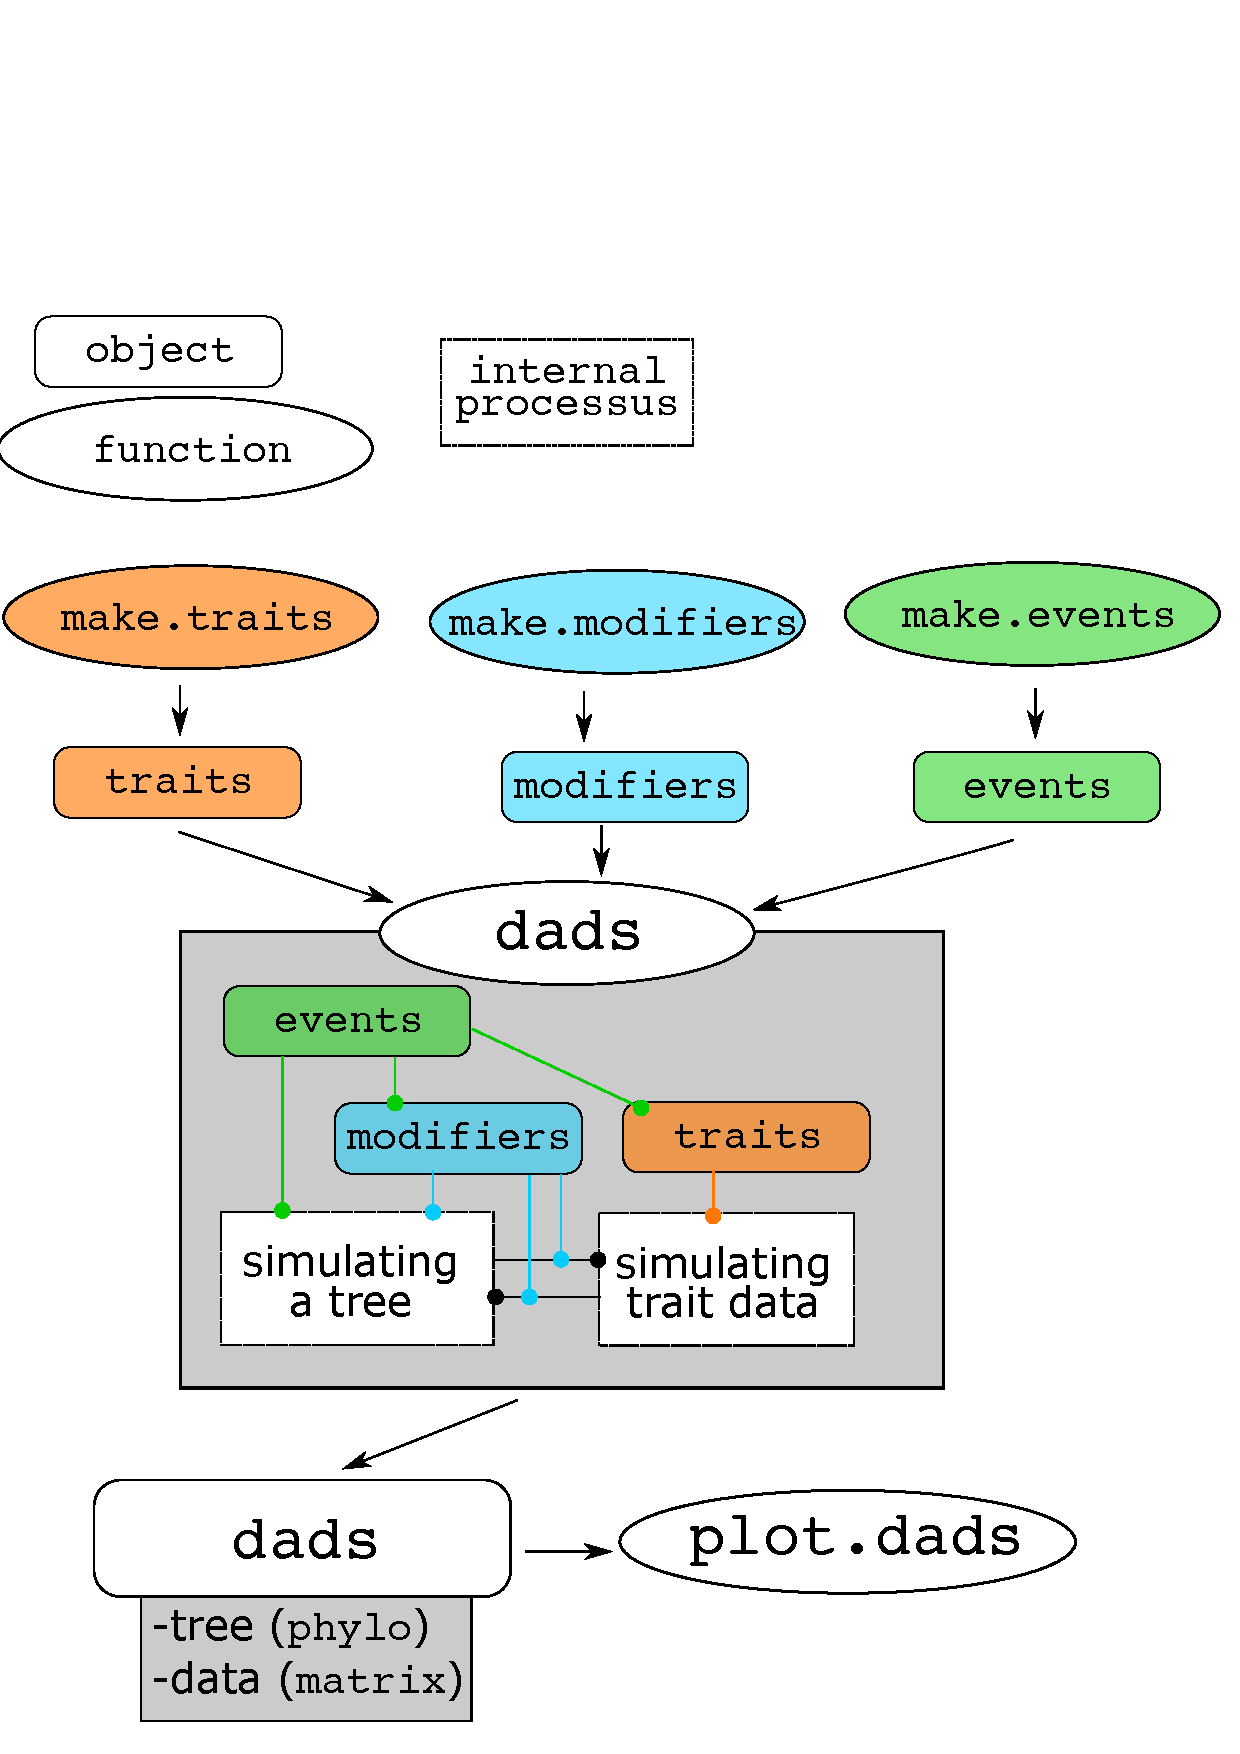
\includegraphics{dads_structure.pdf}
\caption{Schematised summary of the \texttt{dads} package architecture}
\end{figure}

\begin{verbatim}
## Loading required package: dispRity
\end{verbatim}

\hypertarget{getting-started}{%
\chapter{Getting started}\label{getting-started}}

\hypertarget{the-simplest-of-all-analysis-simulating-diversity-only}{%
\section{The simplest of all analysis: simulating diversity only}\label{the-simplest-of-all-analysis-simulating-diversity-only}}

One of the simplest things to do with the \texttt{dads} package is just to simulate a birth death tree.
For that you can use the function \texttt{dads} and specify your stopping rule.
The stopping rule simply tells the birth death process to step whenever it reaches one of these three conditions:

\begin{itemize}
\tightlist
\item
  \texttt{"max.taxa"\ \ \ =\ n} stop when \texttt{n} taxa are generated;
\item
  \texttt{"max.living"\ =\ n} stop when there is \texttt{n} co-occuring taxa of the same age (i.e. ``living'' taxa);
\item
  \texttt{"max.time"\ \ \ =\ n} stop when the simulated tree is \texttt{n} units of age old (these units are arbitrary);
\end{itemize}

For example, we might want to generate a birth-death tree with 20 taxa:

\begin{Shaded}
\begin{Highlighting}[]
\CommentTok{## Setting a stopping rule to reach a maximum of 20 taxa}
\NormalTok{my_stop_rule <-}\StringTok{ }\KeywordTok{list}\NormalTok{(}\DataTypeTok{max.taxa =} \DecValTok{20}\NormalTok{)}
\end{Highlighting}
\end{Shaded}

We can now run the simulations using:

\begin{Shaded}
\begin{Highlighting}[]
\CommentTok{## Running the birth death simulation}
\NormalTok{my_tree <-}\StringTok{ }\KeywordTok{dads}\NormalTok{(}\DataTypeTok{stop.rule =}\NormalTok{ my_stop_rule)}
\end{Highlighting}
\end{Shaded}

\begin{quote}
Note that here we could have specified more than one stopping rule, for example, we might want to run a simulation and stop it if it either reaches 10 taxa or the age 2 using \texttt{stop.rule\ =\ list(max.time\ =\ 2,\ max.taxa\ =\ 10)}. The simulation will then stop when either of these conditions are met.
\end{quote}

The resulting object is a classic \texttt{"phylo"} object that you can simply plot or visualise like so:

\begin{Shaded}
\begin{Highlighting}[]
\CommentTok{## The tree object}
\NormalTok{my_tree}
\end{Highlighting}
\end{Shaded}

\begin{verbatim}
## 
## Phylogenetic tree with 20 tips and 19 internal nodes.
## 
## Tip labels:
##   t1, t2, t3, t4, t5, t6, ...
## Node labels:
##   n1, n2, n3, n4, n5, n6, ...
## 
## Rooted; includes branch lengths.
\end{verbatim}

\begin{Shaded}
\begin{Highlighting}[]
\CommentTok{## Plotting it}
\KeywordTok{plot}\NormalTok{(my_tree)}
\end{Highlighting}
\end{Shaded}

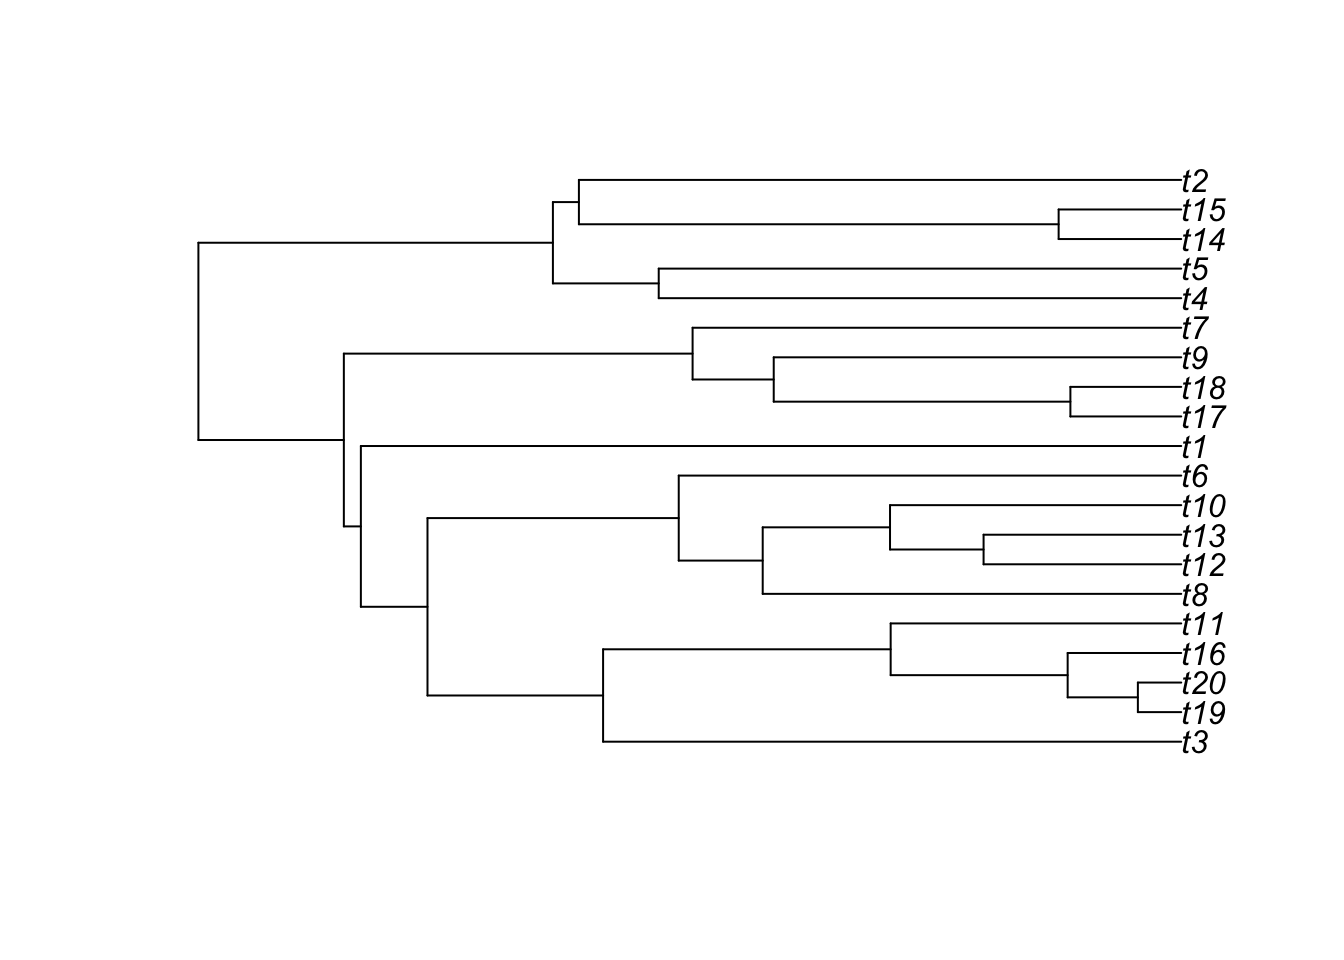
\includegraphics{dads_manual_files/figure-latex/unnamed-chunk-6-1.pdf}

\hypertarget{changing-the-birth-death-parameters}{%
\subsection{Changing the birth-death parameters}\label{changing-the-birth-death-parameters}}

People familiar with the \href{https://lukejharmon.github.io/pcm/chapter10_birthdeath/}{birth-death models} might have noticed that we did not specify two important things here: the speciation parameter (sometimes called ``lambda'' or ``birth'') and the extinction parameter (sometimes called ``mu'', ``death'' or ``background extinction'').
By default \texttt{dads} runs a pure birth model (the speciation is set to 1 and the extinction to 0).
However, you can easily change that by specifying your new birth death parameters:

\begin{Shaded}
\begin{Highlighting}[]
\CommentTok{## my birth death parameters}
\NormalTok{my_params <-}\StringTok{ }\KeywordTok{list}\NormalTok{(}\DataTypeTok{speciation =} \DecValTok{1}\NormalTok{,}
                  \DataTypeTok{extinction =} \DecValTok{1}\OperatorTok{/}\DecValTok{3}\NormalTok{)}
\end{Highlighting}
\end{Shaded}

\begin{quote}
Note that here it is not necessary to specify \texttt{extinction\ =\ 1} since this is the default option, you can always just change the parameter of interest (e.g.~changing \texttt{extinciton\ =\ 0} to \texttt{extinction\ =\ 1/3}). However, we think it's good practice to attribute both parameters specifically to avoid any confusion.
\end{quote}

You can then run the same birth death tree with extinction:

\begin{Shaded}
\begin{Highlighting}[]
\CommentTok{## Generating a birth death tree with extinctions:}
\NormalTok{my_tree <-}\StringTok{ }\KeywordTok{dads}\NormalTok{(}\DataTypeTok{bd.params =}\NormalTok{ my_params, }\DataTypeTok{stop.rule =}\NormalTok{ my_stop_rule)}
\CommentTok{## Visualising the new tree}
\KeywordTok{plot}\NormalTok{(my_tree)}
\end{Highlighting}
\end{Shaded}

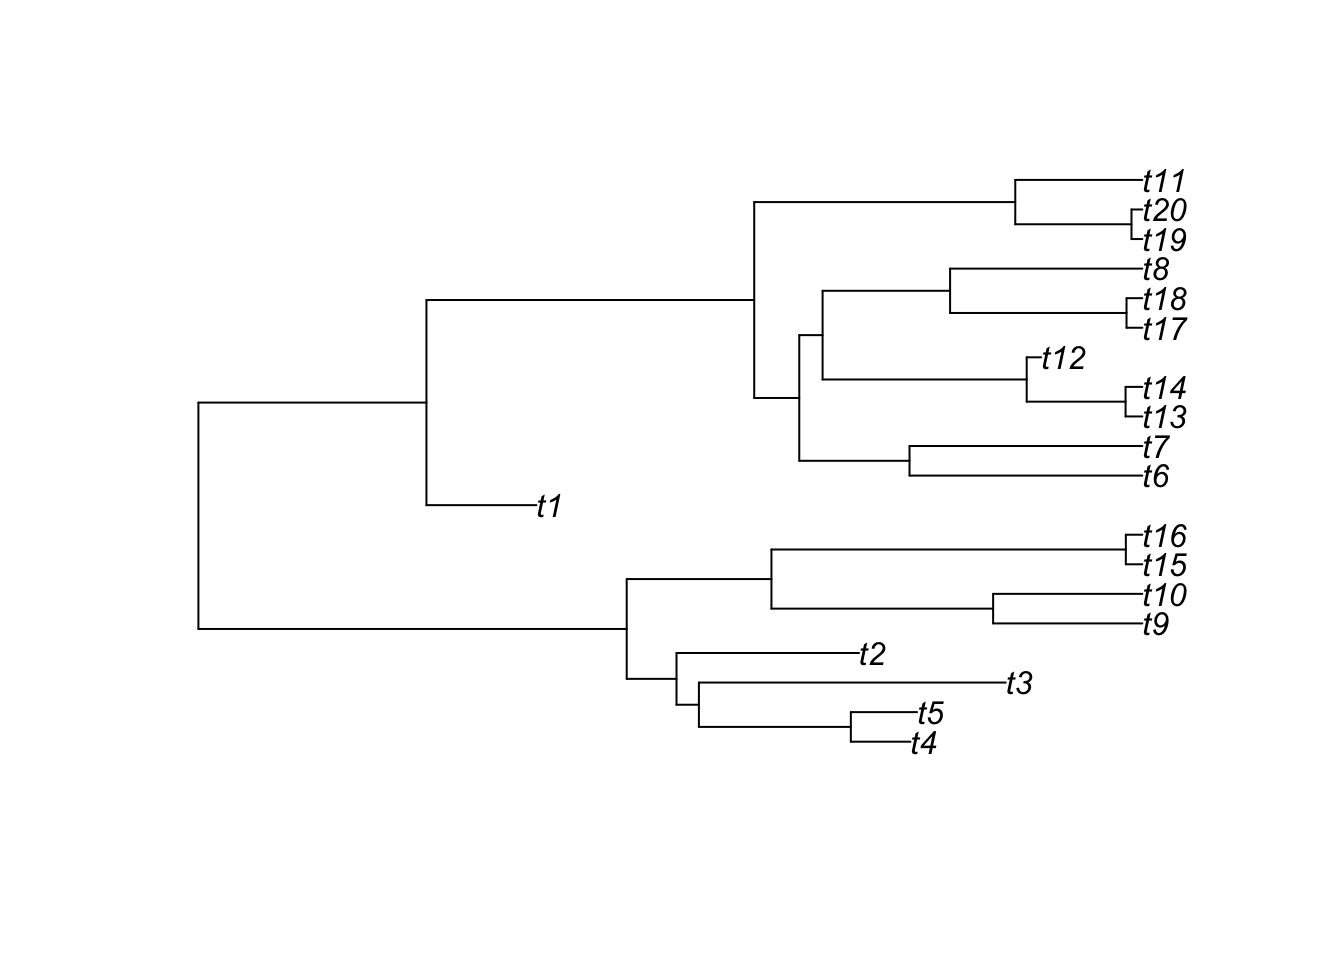
\includegraphics{dads_manual_files/figure-latex/unnamed-chunk-8-1.pdf}

\hypertarget{slightly-more-complex-simulating-disparity-and-diversity}{%
\section{Slightly more complex: simulating disparity and diversity}\label{slightly-more-complex-simulating-disparity-and-diversity}}

Chances are that you want to also simulate traits (disparity) along with your diversity (otherwise, we suggest using the \href{https://github.com/tanja819/TreeSim/}{\texttt{TreeSim}} package that provides many more birth death models).
Simulating traits is not much more complicated in \texttt{dads}: you'll simply need to create a \texttt{"traits"} object using the \texttt{make.traits} function.
These objects can have increasing complexity (see the rest of this tutorial) but we will keep it simple here.

\texttt{"traits"} objects contain one or more processes which are the ways to generate the trait.
The most common of these processes is the \href{https://en.wikipedia.org/wiki/Brownian_motion}{Brownian Motion}.
This is used by default with the \texttt{make.traits} function:

\begin{Shaded}
\begin{Highlighting}[]
\CommentTok{## Creating the traits object}
\NormalTok{my_trait <-}\StringTok{ }\KeywordTok{make.traits}\NormalTok{()}
\end{Highlighting}
\end{Shaded}

This trait object can be simply printed (to see what's in it) or plotted (to see what the process looks like in the absence of a phylogeny):

\begin{Shaded}
\begin{Highlighting}[]
\CommentTok{## Which process is in here?}
\NormalTok{my_trait}
\end{Highlighting}
\end{Shaded}

\begin{verbatim}
##  ---- dads traits object ---- 
## 1 trait for 1 process (A) with one starting value (0).
\end{verbatim}

\begin{Shaded}
\begin{Highlighting}[]
\CommentTok{## What does it look like?}
\KeywordTok{plot}\NormalTok{(my_trait)}
\end{Highlighting}
\end{Shaded}

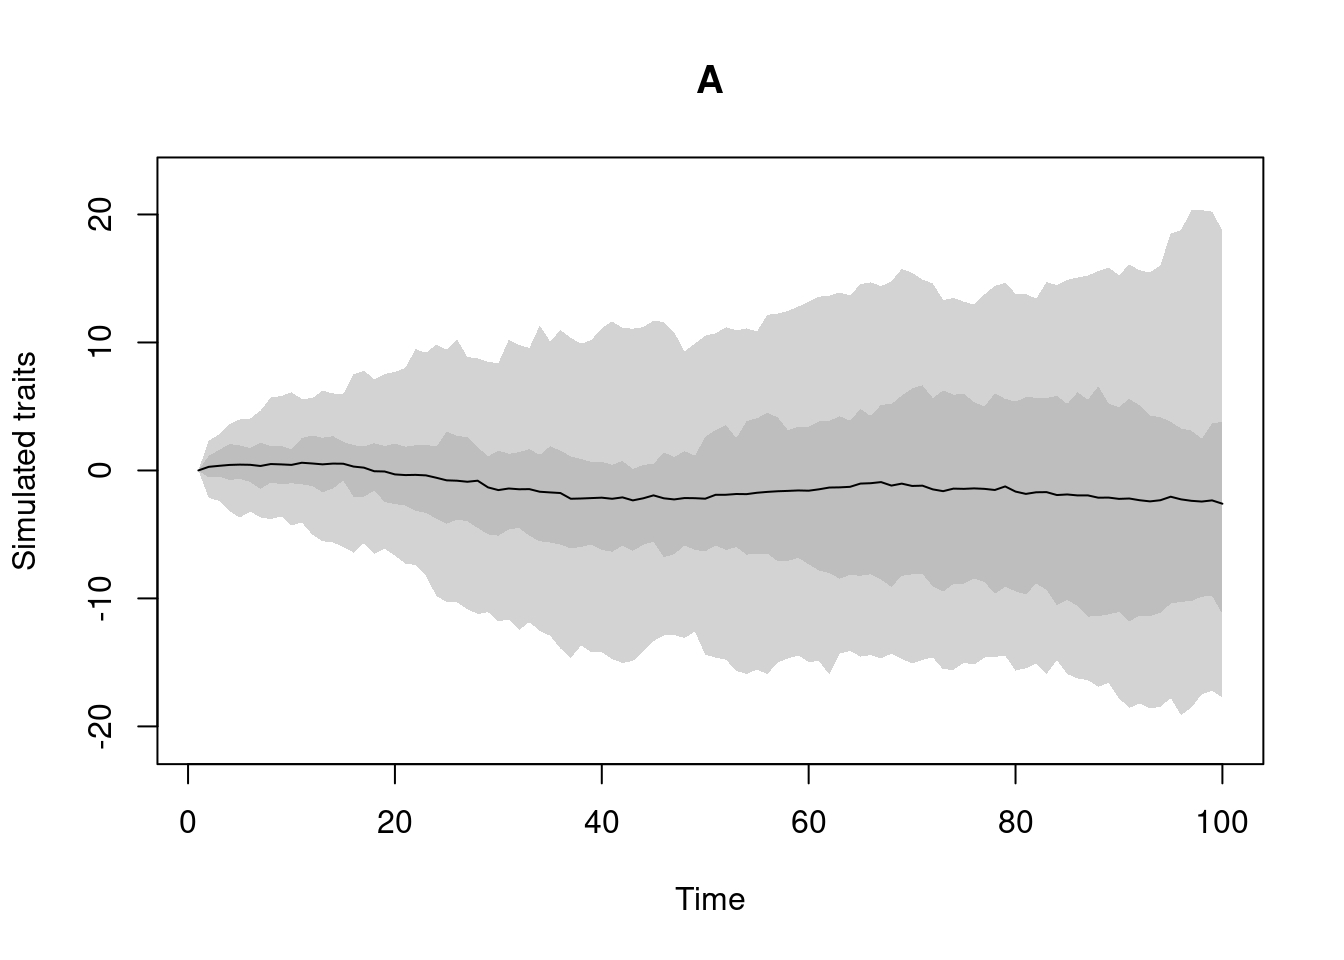
\includegraphics{dads_manual_files/figure-latex/unnamed-chunk-10-1.pdf}

By default, this trait is called ``A''.
This is not a really good name but you'll see more about specifying trait names later on.
If this is what the process should look like (theoretically) you can then add its \texttt{"traits"} object to our previous \texttt{dads} function to generate the tree and the traits:

\begin{Shaded}
\begin{Highlighting}[]
\CommentTok{## Simulate disparity and diversity}
\NormalTok{my_data <-}\StringTok{ }\KeywordTok{dads}\NormalTok{(}\DataTypeTok{bd.params =}\NormalTok{ my_params,}
                \DataTypeTok{stop.rule =}\NormalTok{ my_stop_rule,}
                \DataTypeTok{traits    =}\NormalTok{ my_trait)}
\end{Highlighting}
\end{Shaded}

Et voilà! We now have a simple disparity and diversity simulation.
We can see what's in the results by simply printing it or plotting it:

\begin{Shaded}
\begin{Highlighting}[]
\CommentTok{## What's in there}
\NormalTok{my_data}
\end{Highlighting}
\end{Shaded}

\begin{verbatim}
##  ---- dads object ---- 
## Simulated diversity data (x$tree):
## 
## Phylogenetic tree with 20 tips and 19 internal nodes.
## 
## Tip labels:
##   t1, t2, t3, t4, t5, t6, ...
## Node labels:
##   n1, n2, n3, n4, n5, n6, ...
## 
## Rooted; includes branch lengths.
## 
## Simulated disparity data (x$data):
## 1 trait for 1 process (A) with one starting value (0).
\end{verbatim}

\begin{Shaded}
\begin{Highlighting}[]
\CommentTok{## Plotting the disparity and diversity}
\KeywordTok{plot}\NormalTok{(my_data)}
\end{Highlighting}
\end{Shaded}

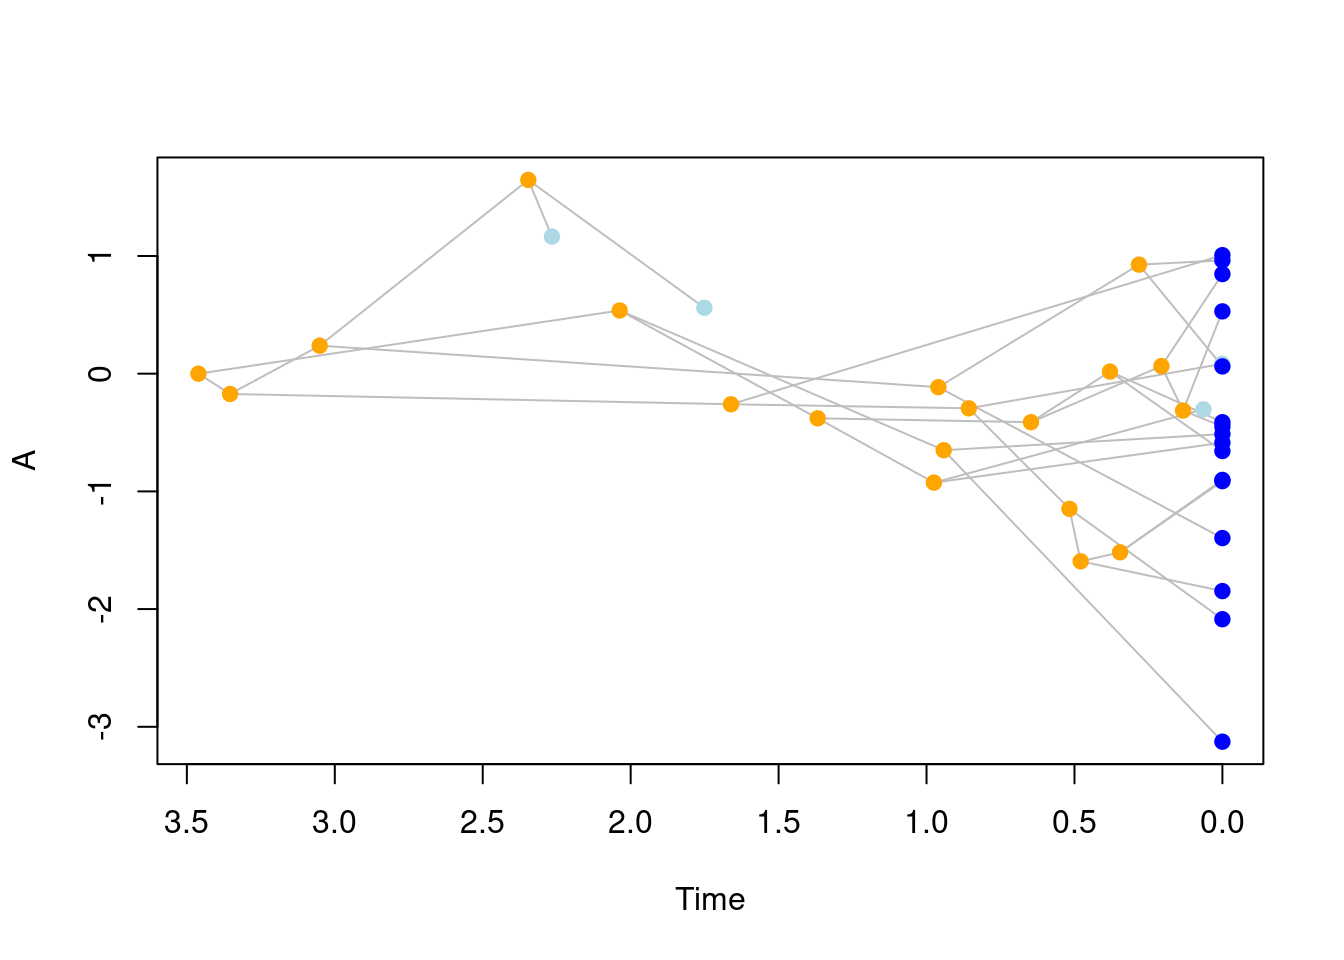
\includegraphics{dads_manual_files/figure-latex/unnamed-chunk-12-1.pdf}

You can then extract the components you need for your specific analysis like so:

\begin{Shaded}
\begin{Highlighting}[]
\CommentTok{## Extracting the tree (a "phylo" object)}
\NormalTok{the_generated_tree <-}\StringTok{ }\NormalTok{my_data}\OperatorTok{$}\NormalTok{tree}
\KeywordTok{class}\NormalTok{(the_generated_tree)}
\end{Highlighting}
\end{Shaded}

\begin{verbatim}
## [1] "phylo"
\end{verbatim}

\begin{Shaded}
\begin{Highlighting}[]
\CommentTok{## Extracting the data (a "matrix")}
\NormalTok{the_generated_data <-}\StringTok{ }\NormalTok{my_data}\OperatorTok{$}\NormalTok{data}
\KeywordTok{class}\NormalTok{(the_generated_data)}
\end{Highlighting}
\end{Shaded}

\begin{verbatim}
## [1] "matrix" "array"
\end{verbatim}

You can find much more on how to design trait objects in the \protect\hyperlink{maketraits}{\texttt{make.traits} section}.

\hypertarget{slightly-more-more-complex-simulating-linked-disparity-and-diversity}{%
\section{Slightly more more complex: simulating linked disparity and diversity}\label{slightly-more-more-complex-simulating-linked-disparity-and-diversity}}

The example above is also still pretty simple and easily done through a variety of \texttt{R} packages: here the trait and the tree are simulated at the same time but only the tree is simulating the trait (i.e.~the trait value at a tip is affected by it's ancestor and the branch length leading to it) but not the other way around (the trait value does not affect the tree).
It is possible to add this aspect using \texttt{"modifiers"} objects.
\texttt{"modifiers"} are similar to \texttt{"traits"} in that you specify what should go in there and then feed it to your simulation.

\texttt{"modifiers"} affect two key steps of the birth-death process: the calculation of the waiting time (i.e.~the component generating branch lengths) and the triggering of speciation or extinction events.
These events can be modified using some \texttt{condition} and \texttt{modify} function.
In other words, when reaching a certain condition specified by a \texttt{condition} function, the birth-death process will modify either the branch length or the speciation (or extinction) probability by applying a \texttt{modify} function.

You can use the function \texttt{make.modifiers} to design a specific \texttt{"modifiers"} object.
By default, this function generates a \texttt{"modifiers"} object that affects branch length and speciation in the following way:

\begin{itemize}
\tightlist
\item
  branch length is a randomly drawn number from an exponential distribution with a rate equal to the current number of taxa multiplied by the sum of the speciation and extinction rates.
\item
  speciation is triggered if a randomly drawn number (from a (0,1) uniform distribution) is smaller than the ratio between the speciation rate and the sum of the speciation and extinction rates. If that random number is greater, the lineage goes extinct.
\end{itemize}

Note that these are default for a birth death tree and were actually already applied in the examples before (without specifying a modifier):

\begin{Shaded}
\begin{Highlighting}[]
\CommentTok{## Make a default modifiers}
\NormalTok{default_modifiers <-}\StringTok{ }\KeywordTok{make.modifiers}\NormalTok{()}
\CommentTok{## What's in it?}
\NormalTok{default_modifiers}
\end{Highlighting}
\end{Shaded}

\begin{verbatim}
##  ---- dads modifiers object ---- 
## No modifiers applied to the branch length, selection and speciation processes (default).
\end{verbatim}

This will not do much to our simulations compared to the previous trait and tree simulation but we can provide our modifiers object to the \texttt{dads} function:

\begin{Shaded}
\begin{Highlighting}[]
\CommentTok{## Setting the simulation parameters}
\NormalTok{extinction_}\DecValTok{02}\NormalTok{ <-}\StringTok{ }\KeywordTok{list}\NormalTok{(}\DataTypeTok{extinction =} \FloatTok{0.2}\NormalTok{)}
\NormalTok{living_}\DecValTok{20}\NormalTok{     <-}\StringTok{ }\KeywordTok{list}\NormalTok{(}\DataTypeTok{max.living =} \DecValTok{20}\NormalTok{)}
\NormalTok{BM_trait      <-}\StringTok{ }\KeywordTok{make.traits}\NormalTok{()}
\KeywordTok{set.seed}\NormalTok{(}\DecValTok{1}\NormalTok{)}
\CommentTok{## Simulate disparity and diversity}
\NormalTok{default_data <-}\StringTok{ }\KeywordTok{dads}\NormalTok{(}\DataTypeTok{bd.params =}\NormalTok{ extinction_}\DecValTok{02}\NormalTok{,}
                     \DataTypeTok{stop.rule =}\NormalTok{ living_}\DecValTok{20}\NormalTok{,}
                     \DataTypeTok{traits    =}\NormalTok{ BM_trait,}
                     \DataTypeTok{modifiers =}\NormalTok{ default_modifiers)}
\NormalTok{default_data}
\end{Highlighting}
\end{Shaded}

\begin{verbatim}
##  ---- dads object ---- 
## Birth death process with modifiers:
## No modifiers applied to the branch length, selection and speciation processes (default).
## 
## Simulated diversity data (x$tree):
## 
## Phylogenetic tree with 24 tips and 23 internal nodes.
## 
## Tip labels:
##   t1, t2, t3, t4, t5, t6, ...
## Node labels:
##   n1, n2, n3, n4, n5, n6, ...
## 
## Rooted; includes branch lengths.
## 
## Simulated disparity data (x$data):
## 1 trait for 1 process (A) with one starting value (0).
\end{verbatim}

Note however that the printing information is now updated to state that you've add a modifier (even though it's a default one).

For more interesting simulations however, you can provide modifiers that actually modify the birth death process.
We can create one for example that makes species go extinct if their ancestor have a negative trait value.
For that we need to create a modifiers object that modifies the \texttt{speciation} process with a specific condition and a specific modification when that condition is met.
First we are going to create the modification function.
This function must intake the argument \texttt{x} and, in our case, return a logical value: \texttt{TRUE} is for speciate and \texttt{FALSE} is for go extinct.
We want this \texttt{modify} function to always return \texttt{FALSE} (go extinct) since it will be triggered by \texttt{condition} (we will see that in a minute).

\begin{Shaded}
\begin{Highlighting}[]
\CommentTok{## Going extinct}
\NormalTok{staying.alive <-}\StringTok{ }\ControlFlowTok{function}\NormalTok{(x) }\KeywordTok{return}\NormalTok{(}\OtherTok{TRUE}\NormalTok{)}
\end{Highlighting}
\end{Shaded}

Now we want this function to only trigger when an ancestor has a negative trait value.
We can do that by specifying our \texttt{condition} function (when the ancestor is trait is negative) apply our modification (here the \texttt{staying.alive} function).
For that we can use the \texttt{parent.traits} utility function that is optimised for accessing traits in the birth death process (but you can of course write your own).
This function intakes the \texttt{trait.values} and \texttt{parent.lineage} arguments, two arguments that you can leave named as they are to facilitate \texttt{dads}s understanding of what you which to asses:

\begin{Shaded}
\begin{Highlighting}[]
\CommentTok{## Triggering a modification only if the ancestor trait is negative}
\NormalTok{negative.ancestor <-}\StringTok{ }\ControlFlowTok{function}\NormalTok{(trait.values, lineage) \{}
    \KeywordTok{return}\NormalTok{(}\KeywordTok{all}\NormalTok{(}\KeywordTok{parent.traits}\NormalTok{(trait.values, lineage) }\OperatorTok{<}\StringTok{ }\DecValTok{0}\NormalTok{))}
\NormalTok{\}}
\end{Highlighting}
\end{Shaded}

Note that we use the function \texttt{all} here to evaluate all traits (if the data is multidimensional).
We can then provide these two functions (the condition \texttt{negative.ancestor} and how to modify the speciation event when this condition is met \texttt{staying.alive}).
If you are an advances \texttt{dads} user, you can design your own \texttt{speciation} function but if you just want to use a normal \texttt{speciation} function, you can use the default one from \texttt{dads} called\ldots{} \texttt{speciation}.

\begin{Shaded}
\begin{Highlighting}[]
\CommentTok{## Making a modifier for species to go extinct if}
\CommentTok{## their ancestor's trait value is (or are) negative}
\NormalTok{negatives_extinct <-}\StringTok{ }\KeywordTok{make.modifiers}\NormalTok{(}
                        \CommentTok{## The speciation function (default)}
                        \DataTypeTok{speciation =}\NormalTok{ speciation,}
                        \CommentTok{## What to modify}
                        \DataTypeTok{modify     =}\NormalTok{ staying.alive,}
                        \CommentTok{## When to modify it}
                        \DataTypeTok{condition  =}\NormalTok{ negative.ancestor)}
\CommentTok{## What's in it?}
\NormalTok{negatives_extinct}
\end{Highlighting}
\end{Shaded}

\begin{verbatim}
##  ---- dads modifiers object ---- 
## Default branch length process.
## Default selection process.
## Speciation process is set to speciation with a condition (negative.ancestor) and a modifier (staying.alive).
\end{verbatim}

Note that the \texttt{make.modifiers} function tests whether the input is compatible with \texttt{dads} by default so unless you have an error message, your \texttt{modifiers} will work!
We can now simulate our tree and traits with our modifier: species will go extinct if their ancestor have a negative trait value:

\begin{Shaded}
\begin{Highlighting}[]
\KeywordTok{set.seed}\NormalTok{(}\DecValTok{1}\NormalTok{)}
\CommentTok{## Simulate disparity and diversity}
\NormalTok{biased_data <-}\StringTok{ }\KeywordTok{dads}\NormalTok{(}\DataTypeTok{bd.params =}\NormalTok{ extinction_}\DecValTok{02}\NormalTok{,}
                    \DataTypeTok{stop.rule =}\NormalTok{ living_}\DecValTok{20}\NormalTok{,}
                    \DataTypeTok{traits    =}\NormalTok{ BM_trait,}
                    \DataTypeTok{modifiers =}\NormalTok{ negatives_extinct)}
\NormalTok{biased_data}
\end{Highlighting}
\end{Shaded}

\begin{verbatim}
##  ---- dads object ---- 
## Birth death process with modifiers:
## Default branch length process.
## Default selection process.
## Speciation process is set to speciation with a condition (negative.ancestor) and a modifier (staying.alive).
## 
## Simulated diversity data (x$tree):
## 
## Phylogenetic tree with 22 tips and 21 internal nodes.
## 
## Tip labels:
##   t1, t2, t3, t4, t5, t6, ...
## Node labels:
##   n1, n2, n3, n4, n5, n6, ...
## 
## Rooted; includes branch lengths.
## 
## Simulated disparity data (x$data):
## 1 trait for 1 process (A) with one starting value (0).
\end{verbatim}

We can now compare the two trees and their trait values.
Note that we've used the same starting seed for both trees so the only thing differing between them is the modifier!
Also, although species

\begin{Shaded}
\begin{Highlighting}[]
\KeywordTok{par}\NormalTok{(}\DataTypeTok{mfrow =} \KeywordTok{c}\NormalTok{(}\DecValTok{1}\NormalTok{,}\DecValTok{2}\NormalTok{))}
\KeywordTok{plot}\NormalTok{(default_data, }\DataTypeTok{main =} \StringTok{"default results"}\NormalTok{)}
\KeywordTok{plot}\NormalTok{(biased_data, }\DataTypeTok{main =} \StringTok{"results with the modifier"}\NormalTok{)}
\end{Highlighting}
\end{Shaded}

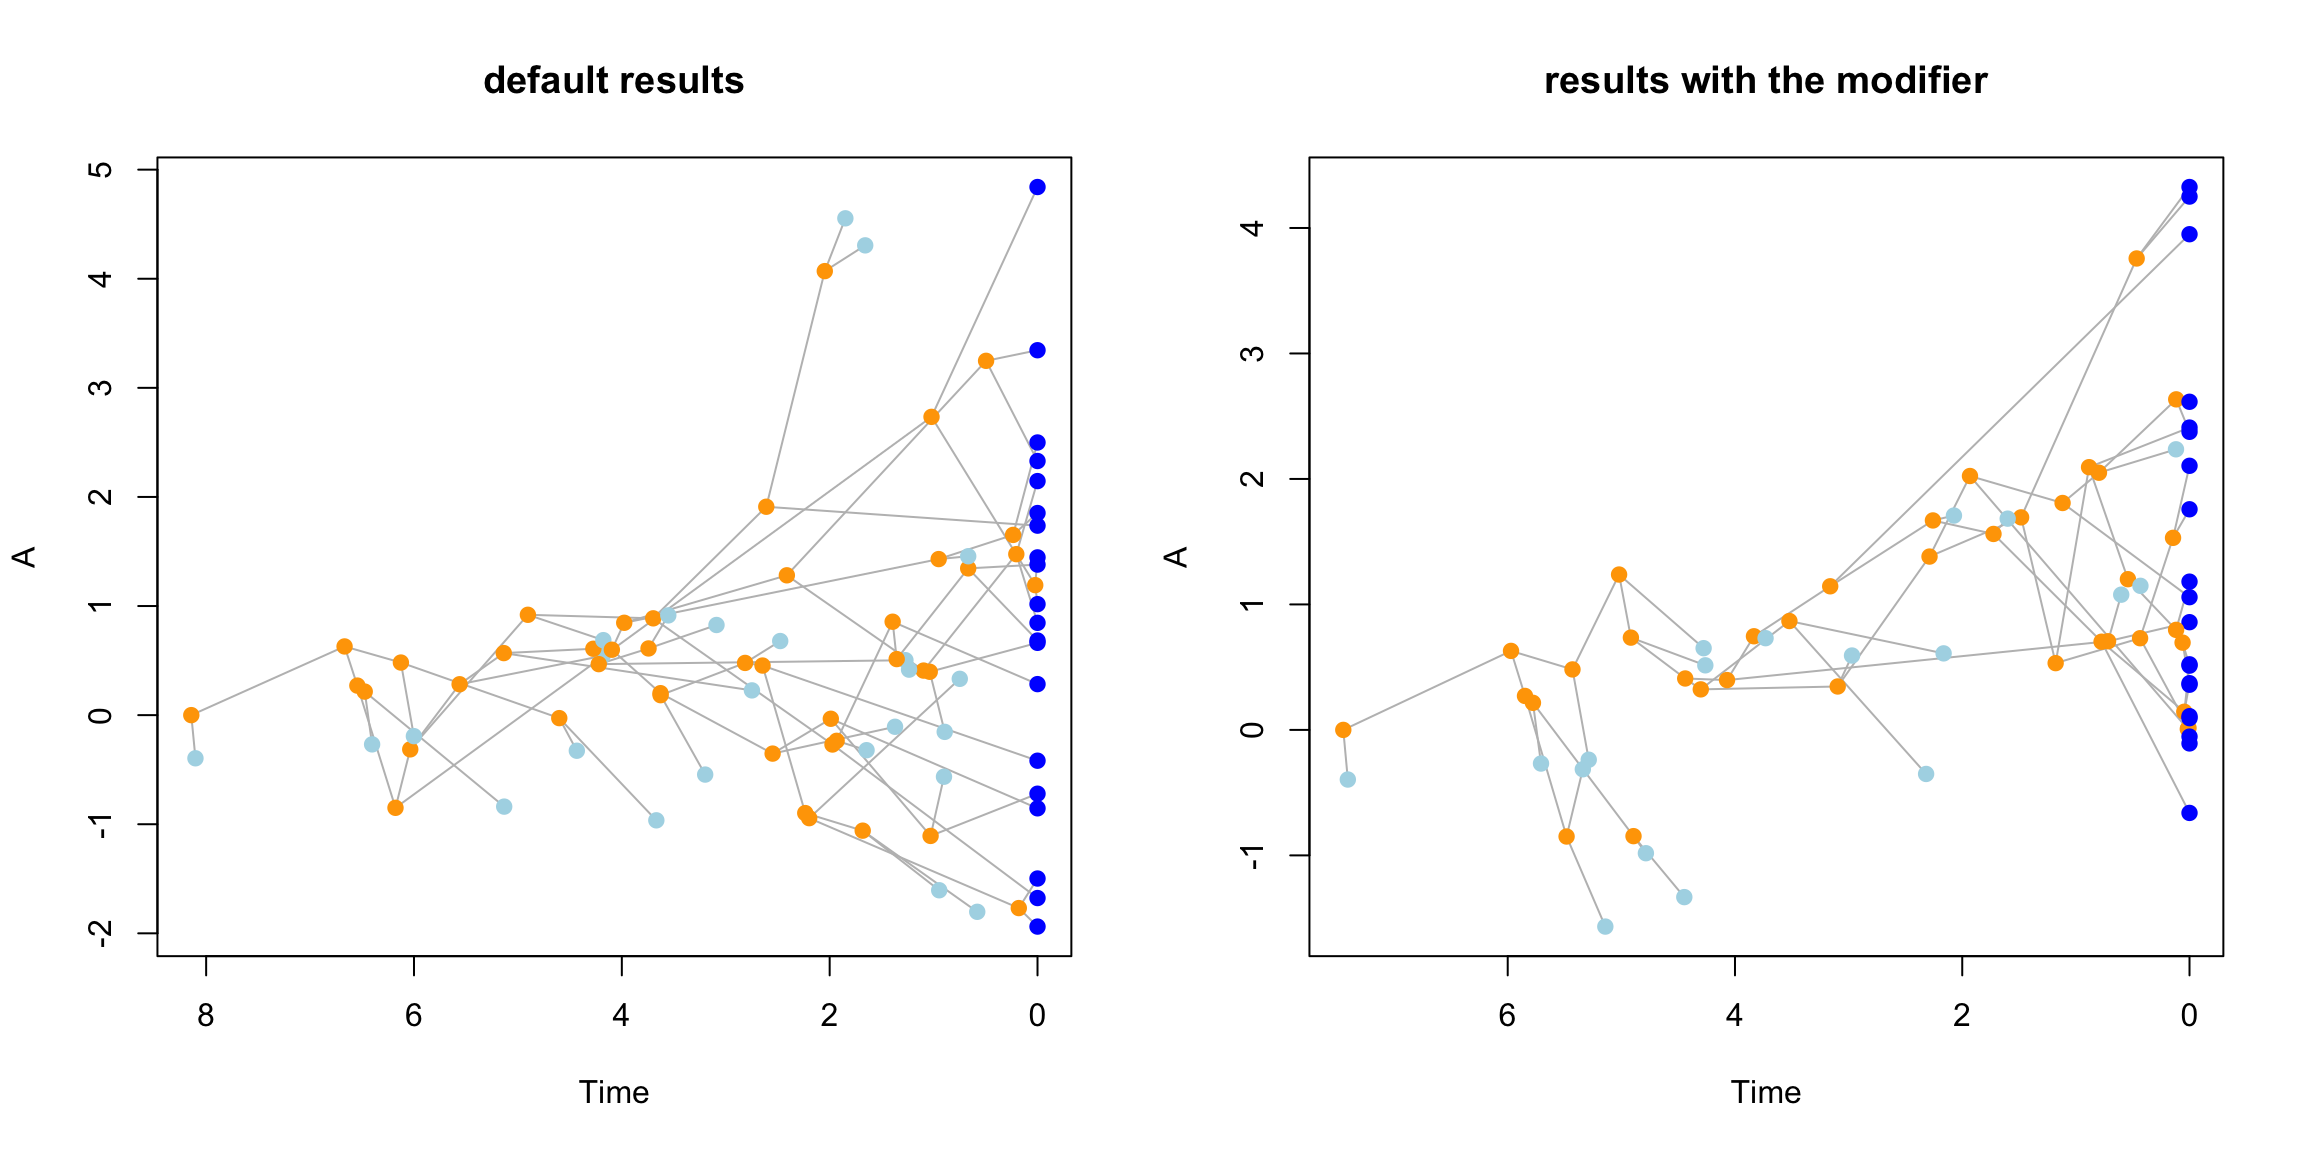
\includegraphics{dads_manual_files/figure-latex/unnamed-chunk-20-1.pdf}

You can find much more how to design modifiers in the \protect\hyperlink{makemodifiers}{\texttt{make.modifiers} section}.

\hypertarget{maketraits}{%
\chapter{\texorpdfstring{Making trait processes with \texttt{make.traits()}}{Making trait processes with make.traits()}}\label{maketraits}}

\hypertarget{the-process-process}{%
\section{\texorpdfstring{The process (\texttt{process})}{The process (process)}}\label{the-process-process}}

The function \texttt{make.traits} allows you to design the process of a trait or a set of traits.
Here, the process of a trait designates the rules to generate the trait through time while simulating a phylogeny.
This process can depend on the previous state in the tree (i.e.~the trait of the ancestor) and the branch length to the descendant.
One classic example is the \href{https://en.wikipedia.org/wiki/Brownian_motion}{Brownian motion process (or Weiner process)}.
Note that it \emph{can} depend on both the ancestor and the branch length but does \emph{not necessary needs} (i.e.~the process can be only based on the previous state or only on branch length or on neither).

Trait processes in \texttt{dads} are functions that must always intake the following arguments by default.

\begin{itemize}
\tightlist
\item
  \texttt{x0}: the previous trait value(s)
\item
  \texttt{edge.length}: the branch length value
\item
  \texttt{...}: a placeholder for any extra arguments
\end{itemize}

For example, the following function would be a valid process (though not dependent on either the previous state nor the branch length):

\begin{Shaded}
\begin{Highlighting}[]
\CommentTok{## A valid (but useless) process}
\NormalTok{valid.process <-}\StringTok{ }\ControlFlowTok{function}\NormalTok{(x0, }\DataTypeTok{egde.length =} \DecValTok{1}\NormalTok{, ...) \{}
    \KeywordTok{return}\NormalTok{(}\DecValTok{42}\NormalTok{)}
\NormalTok{\}}
\end{Highlighting}
\end{Shaded}

\begin{quote}
Note that the argument \texttt{edge.length} is set to \texttt{1} by default. In general we highly recommend to set all arguments but \texttt{x0} to a default value (this really helps the speeding up the \texttt{dads} function).
\end{quote}

On the other hand, the following process (a unidimensional Brownian motion) is incorrect (it's missing \texttt{edge.length} and \texttt{...}):

\begin{Shaded}
\begin{Highlighting}[]
\CommentTok{## A wrongly formated process}
\NormalTok{invalid.process <-}\StringTok{ }\ControlFlowTok{function}\NormalTok{(x0) \{}
    \KeywordTok{return}\NormalTok{(}\KeywordTok{rnorm}\NormalTok{(}\DecValTok{1}\NormalTok{, }\DataTypeTok{mean =}\NormalTok{ x0))}
\NormalTok{\}}
\end{Highlighting}
\end{Shaded}

The \texttt{dads} package proposes inbuilt processes, namely a multidimensional Brownian motion (\texttt{BM.process}) or a a multidimensional Ornstein-Uhlenbeck process (\texttt{OU.process}).
You can find the list of implemented process by looking at the \texttt{?trait.process} manual page in \texttt{R}.

Once a process is chosen, you can feed it to the \texttt{make.traits} function:

\begin{Shaded}
\begin{Highlighting}[]
\CommentTok{## Creating a trait object}
\NormalTok{my_trait_object <-}\StringTok{ }\KeywordTok{make.traits}\NormalTok{(}\DataTypeTok{process =}\NormalTok{ BM.process)}
\end{Highlighting}
\end{Shaded}

This creates \texttt{"dads"} \texttt{"traits"} objects that you can print, and visualise using the \texttt{plot} function:

\begin{Shaded}
\begin{Highlighting}[]
\CommentTok{## The class of the object}
\KeywordTok{class}\NormalTok{(my_trait_object)}
\end{Highlighting}
\end{Shaded}

\begin{verbatim}
## [1] "dads"   "traits"
\end{verbatim}

\begin{Shaded}
\begin{Highlighting}[]
\CommentTok{## What's in it?}
\NormalTok{my_trait_object}
\end{Highlighting}
\end{Shaded}

\begin{verbatim}
##  ---- dads traits object ---- 
## 1 trait for 1 process (A) with one starting value (0).
\end{verbatim}

\begin{Shaded}
\begin{Highlighting}[]
\CommentTok{## What does the process looks like}
\KeywordTok{plot}\NormalTok{(my_trait_object)}
\end{Highlighting}
\end{Shaded}

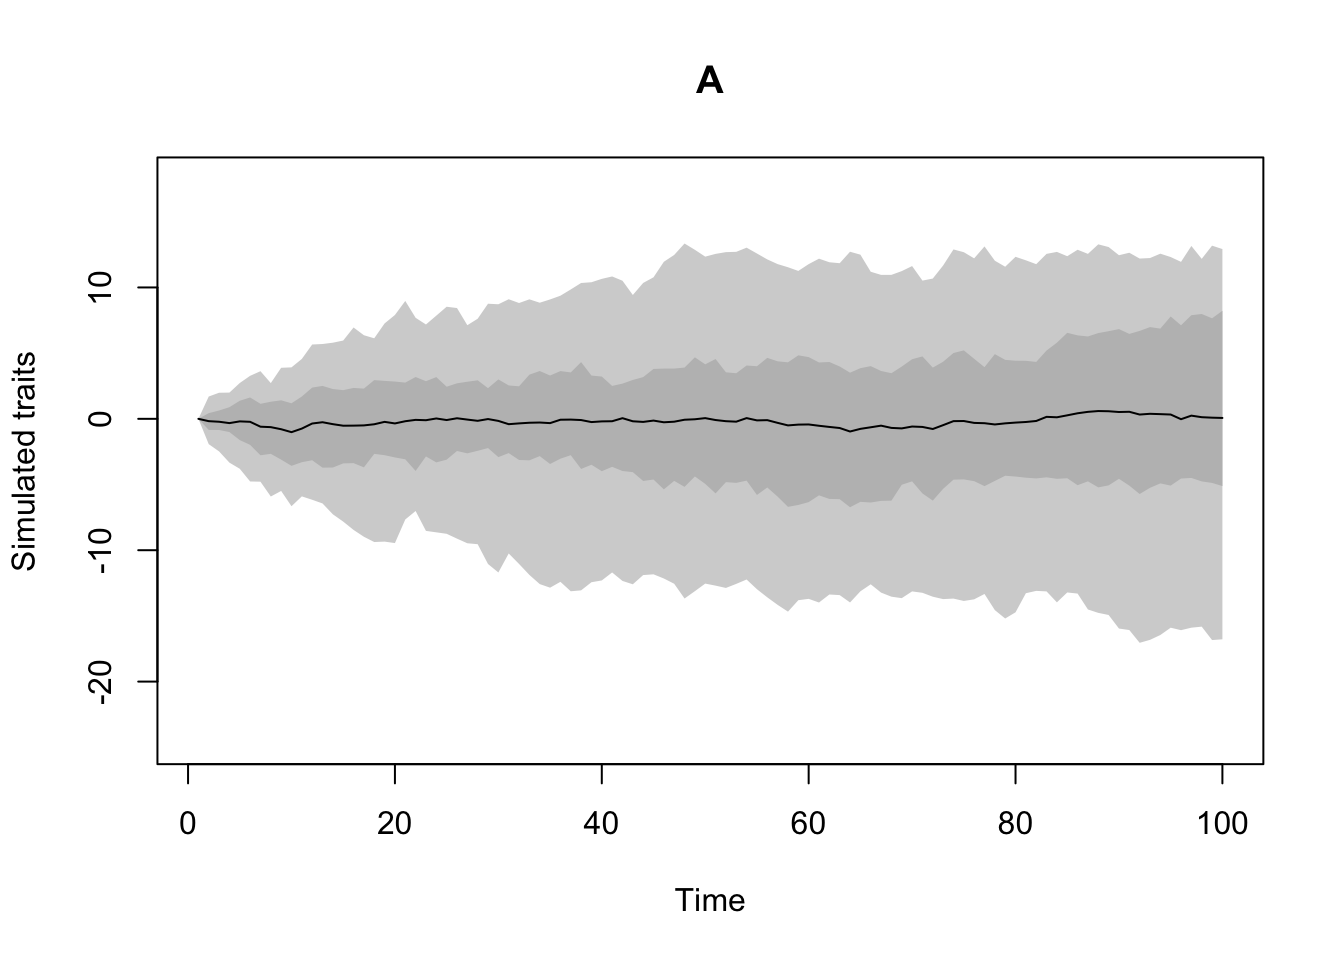
\includegraphics{dads_manual_files/figure-latex/unnamed-chunk-25-1.pdf}

Note that you can see the multiple options for plotting the trait process by looking at \texttt{?plot.dads} manual. Furthermore, you can look at what's actually in the object using:

\begin{Shaded}
\begin{Highlighting}[]
\CommentTok{## What's actually in that object?}
\KeywordTok{print.dads}\NormalTok{(my_trait_object, }\DataTypeTok{all =} \OtherTok{TRUE}\NormalTok{)}
\end{Highlighting}
\end{Shaded}

\begin{verbatim}
## $A
## $A$process
## function (x0, edge.length = 1, Sigma = diag(length(x0)), ...) 
## {
##     return(t(MASS::mvrnorm(n = 1, mu = x0, Sigma = Sigma * edge.length, 
##         ...)))
## }
## <bytecode: 0x7faff6222240>
## <environment: namespace:dads>
## 
## $A$start
## [1] 0
## 
## $A$trait_id
## [1] 1
\end{verbatim}

As traits can get more and more complex, the automatic printing of its summary allows for a easier display of what's in the traits object.

Note that it is possible to make \texttt{"traits"} objects with multiple processes (that can be the same):

\begin{Shaded}
\begin{Highlighting}[]
\CommentTok{## 4 traits: two BM, one OU and one normal non process}
\NormalTok{four_traits <-}\StringTok{ }\KeywordTok{make.traits}\NormalTok{(}\DataTypeTok{process =} \KeywordTok{c}\NormalTok{(BM.process,}
\NormalTok{                                       BM.process,}
\NormalTok{                                       OU.process,}
\NormalTok{                                       no.process))}
\NormalTok{four_traits}
\end{Highlighting}
\end{Shaded}

\begin{verbatim}
##  ---- dads traits object ---- 
## 4 traits for 4 processes (A, B, C, D) with one starting value (0).
\end{verbatim}

You can visualise them individually using the \texttt{trait} argument in \texttt{plot.dads}:

\begin{Shaded}
\begin{Highlighting}[]
\CommentTok{## Plot options (4 plots in one window)}
\KeywordTok{par}\NormalTok{(}\DataTypeTok{mfrow =} \KeywordTok{c}\NormalTok{(}\DecValTok{2}\NormalTok{,}\DecValTok{2}\NormalTok{))}
\KeywordTok{plot}\NormalTok{(four_traits, }\DataTypeTok{trait =} \DecValTok{1}\NormalTok{)}
\KeywordTok{plot}\NormalTok{(four_traits, }\DataTypeTok{trait =} \DecValTok{2}\NormalTok{)}
\KeywordTok{plot}\NormalTok{(four_traits, }\DataTypeTok{trait =} \DecValTok{3}\NormalTok{)}
\KeywordTok{plot}\NormalTok{(four_traits, }\DataTypeTok{trait =} \DecValTok{4}\NormalTok{)}
\end{Highlighting}
\end{Shaded}

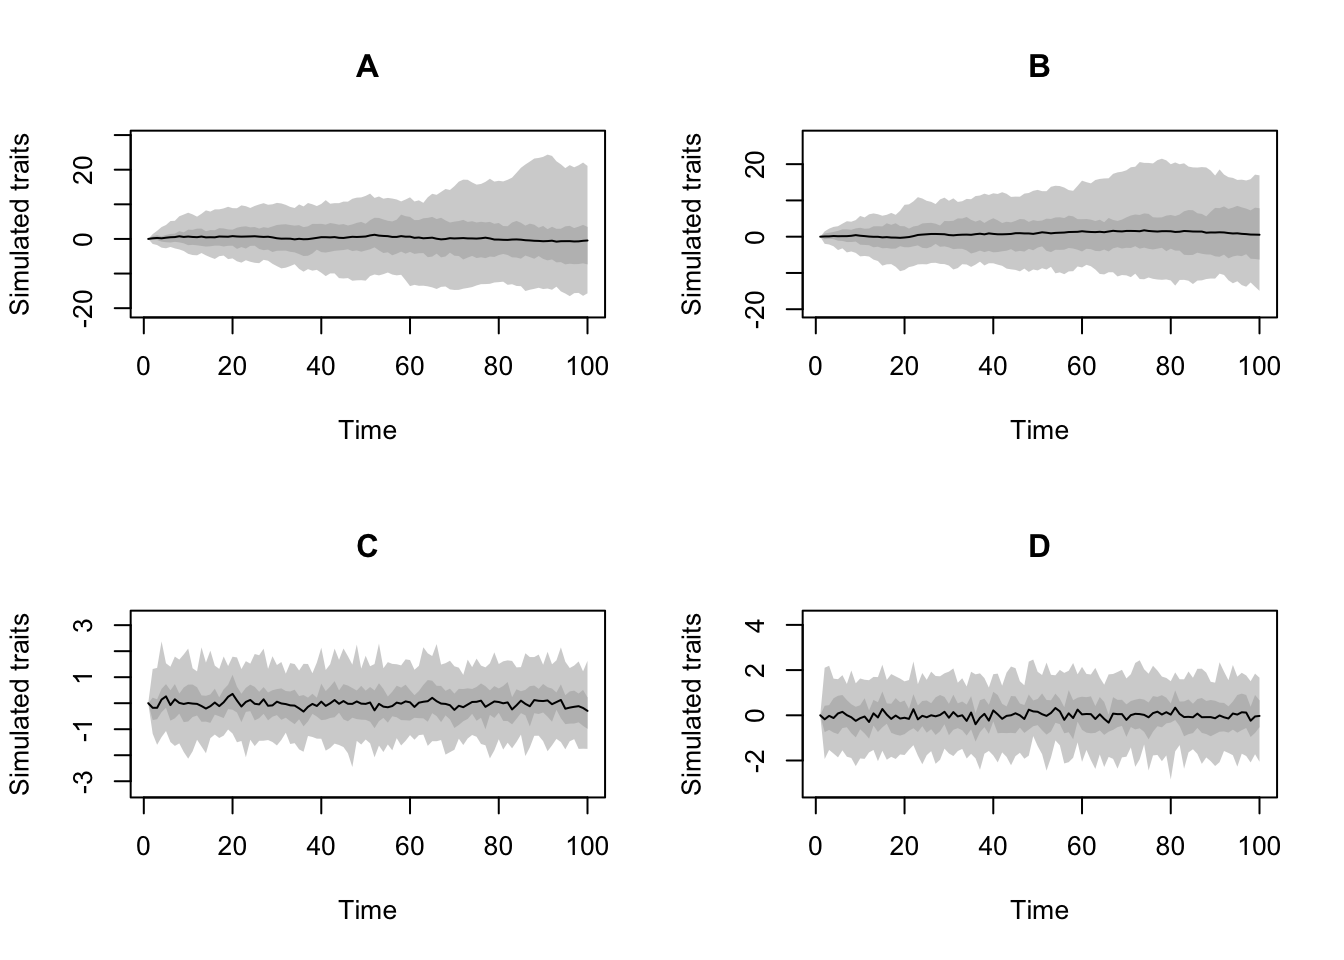
\includegraphics{dads_manual_files/figure-latex/unnamed-chunk-28-1.pdf}

\hypertarget{the-number-of-traits-n-and-the-starting-values-start}{%
\section{\texorpdfstring{The number of traits \texttt{n} and the starting values \texttt{start}}{The number of traits n and the starting values start}}\label{the-number-of-traits-n-and-the-starting-values-start}}

Two further important arguments are \texttt{n} the number of traits per process and \texttt{start} the starting values for all traits.
By default they are set to \texttt{n\ =\ 1} and \texttt{start\ =\ 0}.
This means that \texttt{make.traits} will assume that your processes are always unidimensional by default and that they always start with the value \texttt{0}.
It is however possible to change these values.

For example you can use the following to create a three dimensional Brownian motion with each dimensions starting with the value \texttt{1}:

\begin{Shaded}
\begin{Highlighting}[]
\CommentTok{## Multidimensional Brownian motion}
\KeywordTok{make.traits}\NormalTok{(BM.process, }\DataTypeTok{n =} \DecValTok{3}\NormalTok{, }\DataTypeTok{start =} \DecValTok{1}\NormalTok{)}
\end{Highlighting}
\end{Shaded}

\begin{verbatim}
##  ---- dads traits object ---- 
## 3 traits for 1 process (A:3) with one starting value (1).
\end{verbatim}

Or the following with each dimensions starting with different values (respectively \texttt{1}, \texttt{2} and \texttt{3}):

\begin{Shaded}
\begin{Highlighting}[]
\CommentTok{## Multidimensional Brownian motion}
\KeywordTok{make.traits}\NormalTok{(BM.process, }\DataTypeTok{n =} \DecValTok{3}\NormalTok{, }\DataTypeTok{start =} \KeywordTok{c}\NormalTok{(}\DecValTok{1}\NormalTok{,}\DecValTok{2}\NormalTok{,}\DecValTok{3}\NormalTok{))}
\end{Highlighting}
\end{Shaded}

\begin{verbatim}
##  ---- dads traits object ---- 
## 3 traits for 1 process (A:3) with different starting values (1,2,3).
\end{verbatim}

Note that the number of traits are distributed per processes.
If the traits contains multiple process, the number of traits are distributed per processes:

\begin{Shaded}
\begin{Highlighting}[]
\CommentTok{## two 3D processes (BM and OU)}
\KeywordTok{make.traits}\NormalTok{(}\KeywordTok{c}\NormalTok{(BM.process, OU.process), }\DataTypeTok{n =} \DecValTok{3}\NormalTok{)}
\end{Highlighting}
\end{Shaded}

\begin{verbatim}
##  ---- dads traits object ---- 
## 6 traits for 2 processes (A:3, B:3) with one starting value (0).
\end{verbatim}

\begin{Shaded}
\begin{Highlighting}[]
\CommentTok{## one 1D processes (BM) and one 4D process (OU)}
\KeywordTok{make.traits}\NormalTok{(}\KeywordTok{c}\NormalTok{(BM.process, OU.process), }\DataTypeTok{n =} \KeywordTok{c}\NormalTok{(}\DecValTok{1}\NormalTok{, }\DecValTok{4}\NormalTok{))}
\end{Highlighting}
\end{Shaded}

\begin{verbatim}
##  ---- dads traits object ---- 
## 5 traits for 2 processes (A:1, B:4) with one starting value (0).
\end{verbatim}

And starting values are distributed for all the traits or for the traits one by one:

\begin{Shaded}
\begin{Highlighting}[]
\CommentTok{## two 3D processes (BM and OU) starting with 1}
\KeywordTok{make.traits}\NormalTok{(}\KeywordTok{c}\NormalTok{(BM.process, OU.process), }\DataTypeTok{n =} \DecValTok{3}\NormalTok{, }\DataTypeTok{start =} \DecValTok{1}\NormalTok{)}
\end{Highlighting}
\end{Shaded}

\begin{verbatim}
##  ---- dads traits object ---- 
## 6 traits for 2 processes (A:3, B:3) with one starting value (1).
\end{verbatim}

\begin{Shaded}
\begin{Highlighting}[]
\CommentTok{## two 3D processes (BM and OU) starting with values 1 to 6}
\KeywordTok{make.traits}\NormalTok{(}\KeywordTok{c}\NormalTok{(BM.process, OU.process), }\DataTypeTok{n =} \DecValTok{3}\NormalTok{, }\DataTypeTok{start =} \DecValTok{1}\OperatorTok{:}\DecValTok{6}\NormalTok{)}
\end{Highlighting}
\end{Shaded}

\begin{verbatim}
##  ---- dads traits object ---- 
## 6 traits for 2 processes (A:3, B:3) with different starting values (1,2,3,4,5,6).
\end{verbatim}

\begin{Shaded}
\begin{Highlighting}[]
\CommentTok{## two 3D processes (BM and OU) with the two first ones starting}
\CommentTok{## with 1 and the 4 other ones with the default (0)}
\KeywordTok{make.traits}\NormalTok{(}\KeywordTok{c}\NormalTok{(BM.process, OU.process), }\DataTypeTok{n =} \DecValTok{3}\NormalTok{, }\DataTypeTok{start =} \KeywordTok{c}\NormalTok{(}\DecValTok{1}\NormalTok{,}\DecValTok{1}\NormalTok{))}
\end{Highlighting}
\end{Shaded}

\begin{verbatim}
## Warning in make.traits(c(BM.process, OU.process), n = 3, start = c(1, 1)): Only
## the first 2 starting values were supplied for a required 6 traits. The missing
## start values are set to 0.
\end{verbatim}

\begin{verbatim}
##  ---- dads traits object ---- 
## 6 traits for 2 processes (A:3, B:3) with different starting values (1,1,0,0,0,0).
\end{verbatim}

\hypertarget{extra-argument-for-the-processes-with-process.args}{%
\section{\texorpdfstring{Extra argument for the processes with \texttt{process.args}}{Extra argument for the processes with process.args}}\label{extra-argument-for-the-processes-with-process.args}}

You can also feed extra arguments to your process(es) functions. For example, the inbuilt process \texttt{no.process} (that is just a number generator not based on the previous value \texttt{x0} or the branch length) can intake a specific random number generator as a function:

\begin{Shaded}
\begin{Highlighting}[]
\CommentTok{## no process trait using the normal distribution (default)}
\KeywordTok{make.traits}\NormalTok{(no.process, }\DataTypeTok{process.args =} \KeywordTok{list}\NormalTok{(}\DataTypeTok{fun =}\NormalTok{ rnorm))}
\end{Highlighting}
\end{Shaded}

\begin{verbatim}
##  ---- dads traits object ---- 
## 1 trait for 1 process (A) with one starting value (0).
## process A uses the following extra argument: fun;
\end{verbatim}

\begin{Shaded}
\begin{Highlighting}[]
\CommentTok{## no process trait using the uniform distribution}
\CommentTok{## bounded between 1 and 100}
\KeywordTok{make.traits}\NormalTok{(no.process, }\DataTypeTok{process.args =} \KeywordTok{list}\NormalTok{(}\DataTypeTok{fun =}\NormalTok{ runif, }\DataTypeTok{min =} \DecValTok{1}\NormalTok{, }\DataTypeTok{max =} \DecValTok{100}\NormalTok{))}
\end{Highlighting}
\end{Shaded}

\begin{verbatim}
##  ---- dads traits object ---- 
## 1 trait for 1 process (A) with one starting value (0).
## process A uses the following extra arguments: fun,min,max;
\end{verbatim}

You can also add multiple extra arguments for multiple processes giving them as a list.

\begin{Shaded}
\begin{Highlighting}[]
\CommentTok{## Two traits with no process:one normal and one uniform (1,100)}
\KeywordTok{make.traits}\NormalTok{(}\DataTypeTok{process      =} \KeywordTok{c}\NormalTok{(no.process, no.process),}
            \DataTypeTok{process.args =} \KeywordTok{list}\NormalTok{(}\KeywordTok{list}\NormalTok{(}\DataTypeTok{fun =}\NormalTok{ rnorm),}
                                \KeywordTok{list}\NormalTok{(}\DataTypeTok{fun =}\NormalTok{ runif, }\DataTypeTok{min =} \DecValTok{1}\NormalTok{, }\DataTypeTok{max =} \DecValTok{100}\NormalTok{)))}
\end{Highlighting}
\end{Shaded}

\begin{verbatim}
##  ---- dads traits object ---- 
## 2 traits for 2 processes (A, B) with one starting value (0).
## process A uses the following extra argument: fun;
## process B uses the following extra arguments: fun,min,max;
\end{verbatim}

If one process do not need extra argument you must still give it and extra \texttt{NULL} process argument:

\begin{Shaded}
\begin{Highlighting}[]
\CommentTok{## Three traits with no process:}
\CommentTok{## one default, one lognormal and one uniform (1,100)}
\KeywordTok{make.traits}\NormalTok{(}\DataTypeTok{process      =} \KeywordTok{c}\NormalTok{(no.process, no.process, no.process),}
            \DataTypeTok{process.args =} \KeywordTok{list}\NormalTok{(}\CommentTok{## Extra arguments for the first process (none)}
                                \KeywordTok{list}\NormalTok{(}\OtherTok{NULL}\NormalTok{),}
                                \CommentTok{## Extra arguments for the second process}
                                \KeywordTok{list}\NormalTok{(}\DataTypeTok{fun =}\NormalTok{ rlnorm),}
                                \CommentTok{## Extra arguments for the third process}
                                \KeywordTok{list}\NormalTok{(}\DataTypeTok{fun =}\NormalTok{ runif, }\DataTypeTok{min =} \DecValTok{1}\NormalTok{, }\DataTypeTok{max =} \DecValTok{100}\NormalTok{)))}
\end{Highlighting}
\end{Shaded}

\begin{verbatim}
##  ---- dads traits object ---- 
## 3 traits for 3 processes (A, B, C) with one starting value (0).
## process B uses the following extra argument: fun;
## process C uses the following extra arguments: fun,min,max;
\end{verbatim}

\hypertarget{naming-the-traits-with-trait.names}{%
\section{\texorpdfstring{Naming the traits with \texttt{trait.names}}{Naming the traits with trait.names}}\label{naming-the-traits-with-trait.names}}

As traits become more and more complex, it can be useful to give clearer names to each process.
This is easily done using the \texttt{trait.names} argument that attributes one name per process:

\begin{Shaded}
\begin{Highlighting}[]
\CommentTok{## A simple trait with a proper name}
\NormalTok{simple_trait <-}\StringTok{ }\KeywordTok{make.traits}\NormalTok{(}\DataTypeTok{trait.names =} \StringTok{"1D Brownian Motion"}\NormalTok{)}
\NormalTok{simple_trait}
\end{Highlighting}
\end{Shaded}

\begin{verbatim}
##  ---- dads traits object ---- 
## 1 trait for 1 process (1D Brownian Motion) with one starting value (0).
\end{verbatim}

This becomes more useful if we use the complex example above:

\begin{Shaded}
\begin{Highlighting}[]
\CommentTok{## Three named traits with no process:}
\CommentTok{## one default, one lognormal and one uniform (1,100)}
\KeywordTok{make.traits}\NormalTok{(}\DataTypeTok{process      =} \KeywordTok{c}\NormalTok{(no.process, no.process, no.process),}
            \DataTypeTok{process.args =} \KeywordTok{list}\NormalTok{(}\CommentTok{## Extra arguments for the first process (none)}
                                \KeywordTok{list}\NormalTok{(}\OtherTok{NULL}\NormalTok{),}
                                \CommentTok{## Extra arguments for the second process}
                                \KeywordTok{list}\NormalTok{(}\DataTypeTok{fun =}\NormalTok{ rlnorm),}
                                \CommentTok{## Extra arguments for the third process}
                                \KeywordTok{list}\NormalTok{(}\DataTypeTok{fun =}\NormalTok{ runif, }\DataTypeTok{min =} \DecValTok{1}\NormalTok{, }\DataTypeTok{max =} \DecValTok{100}\NormalTok{)),}
            \CommentTok{## Naming each trait}
            \DataTypeTok{trait.names  =} \KeywordTok{c}\NormalTok{(}\StringTok{"Normal"}\NormalTok{, }\StringTok{"LogNormal"}\NormalTok{, }\StringTok{"Uniform(1,100)"}\NormalTok{))}
\end{Highlighting}
\end{Shaded}

\begin{verbatim}
##  ---- dads traits object ---- 
## 3 traits for 3 processes (Normal, LogNormal, Uniform(1,100)) with one starting value (0).
## process LogNormal uses the following extra argument: fun;
## process Uniform(1,100) uses the following extra arguments: fun,min,max;
\end{verbatim}

\hypertarget{combining-multiple-traits-with-add}{%
\section{\texorpdfstring{Combining multiple traits with \texttt{add}}{Combining multiple traits with add}}\label{combining-multiple-traits-with-add}}

You can also add traits to already existing trait objects using the simple \texttt{add} option.
This option just intakes a \texttt{"dads"} \texttt{"traits"} object and the additional process(es) will be added to it. For example:

\begin{Shaded}
\begin{Highlighting}[]
\CommentTok{## Creating on simple default Brownian motion}
\NormalTok{one_process <-}\StringTok{ }\KeywordTok{make.traits}\NormalTok{(}\DataTypeTok{trait.names =} \StringTok{"BM"}\NormalTok{)}

\CommentTok{## Creating a new trait (a 3D OU.process)}
\CommentTok{## and adding the previous one}
\NormalTok{two_processes <-}\StringTok{ }\KeywordTok{make.traits}\NormalTok{(OU.process, }\DataTypeTok{n =} \DecValTok{3}\NormalTok{, }\DataTypeTok{add =}\NormalTok{ one_process,}
                             \DataTypeTok{trait.names =} \StringTok{"3D OU"}\NormalTok{)}

\CommentTok{## Only one process}
\NormalTok{one_process}
\end{Highlighting}
\end{Shaded}

\begin{verbatim}
##  ---- dads traits object ---- 
## 1 trait for 1 process (BM) with one starting value (0).
\end{verbatim}

\begin{Shaded}
\begin{Highlighting}[]
\CommentTok{## The two processes}
\NormalTok{two_processes}
\end{Highlighting}
\end{Shaded}

\begin{verbatim}
##  ---- dads traits object ---- 
## 4 traits for 2 processes (BM:1, 3D OU:3) with one starting value (0).
\end{verbatim}

\hypertarget{testing-the-traits-with-test}{%
\section{\texorpdfstring{Testing the traits with \texttt{test}}{Testing the traits with test}}\label{testing-the-traits-with-test}}

This bit is more for development.
We highly suggest leaving \texttt{test\ =\ TRUE} so that \texttt{make.traits} returns an error if a process or its additional arguments (\texttt{process.args}) are not formatted correctly.
\texttt{make.traits} will error if the trait cannot be directly passed to \texttt{dads}.
However, in some specific cases (again, probably mainly for development and debugging) it could be useful to skip the tests using \texttt{test\ =\ FALSE}.

\hypertarget{templates-for-making-your-very-own-process}{%
\section{Templates for making your very own process}\label{templates-for-making-your-very-own-process}}

As detailed above, any process of your own design will work as long as it is a function that takes at least the arguments \texttt{x0} and \texttt{edge.length}.
You can be imaginative and creative when designing your own process but here are two detailed example functions for a unidimensional Brownian Motion and Ornstein-Uhlenbeck process that you can use for a start (or not).
Remember it is good practice for \texttt{dads} processes to set all the arguments but \texttt{x0} with default values (just in case).
Also, note that the functions below are not equal to the already implemented \texttt{BM.process} and \texttt{OU.process} but are rather generalised/simplified version that you can use as a template

\hypertarget{a-simple-brownian-motion-process-template}{%
\subsection{A simple Brownian Motion process template}\label{a-simple-brownian-motion-process-template}}

\begin{Shaded}
\begin{Highlighting}[]
\CommentTok{## A simple Brownian motion process}
\NormalTok{my.BM.process <-}\StringTok{ }\ControlFlowTok{function}\NormalTok{(x0, }\DataTypeTok{edge.length =} \DecValTok{1}\NormalTok{, }\DataTypeTok{sd =} \DecValTok{1}\NormalTok{, ...) \{}
    \CommentTok{## Drawing a random number from a normal distribution}
    \CommentTok{## with x0 as the and a given standard deviation}
    \CommentTok{## and depending on branch (edge) length}
\NormalTok{    result <-}\StringTok{ }\KeywordTok{rnorm}\NormalTok{(}\DataTypeTok{n =} \DecValTok{1}\NormalTok{, }\DataTypeTok{mean =}\NormalTok{ x0, }\DataTypeTok{sd =}\NormalTok{ sd }\OperatorTok{*}\StringTok{ }\NormalTok{edge.length)}

    \CommentTok{## Return the number}
    \KeywordTok{return}\NormalTok{(result)}
\NormalTok{\}}
\end{Highlighting}
\end{Shaded}

\hypertarget{a-simple-ornstein-uhlenbeck-process-template}{%
\subsection{A simple Ornstein-Uhlenbeck process template}\label{a-simple-ornstein-uhlenbeck-process-template}}

\begin{Shaded}
\begin{Highlighting}[]
\CommentTok{## A simple Ornstein-Uhlenbeck motion process}
\NormalTok{my.OU.process <-}\StringTok{ }\ControlFlowTok{function}\NormalTok{(x0, }\DataTypeTok{edge.length =} \DecValTok{1}\NormalTok{, }\DataTypeTok{var =} \DecValTok{1}\NormalTok{, }\DataTypeTok{alpha =} \DecValTok{1}\NormalTok{, ...) \{}
    \CommentTok{## Calculate the mean based on alpha}
\NormalTok{    mean <-}\StringTok{ }\NormalTok{x0 }\OperatorTok{*}\StringTok{ }\KeywordTok{exp}\NormalTok{(}\OperatorTok{-}\NormalTok{alpha)}
    \CommentTok{## Calculate the standard deviation based on alpha and the variance}
\NormalTok{    sd <-}\StringTok{ }\KeywordTok{sqrt}\NormalTok{(var}\OperatorTok{/}\NormalTok{(}\DecValTok{2} \OperatorTok{*}\StringTok{ }\NormalTok{alpha) }\OperatorTok{*}\StringTok{ }\NormalTok{(}\DecValTok{1} \OperatorTok{-}\StringTok{ }\KeywordTok{exp}\NormalTok{(}\OperatorTok{-}\DecValTok{2} \OperatorTok{*}\StringTok{ }\NormalTok{alpha)))}
    \CommentTok{## Draw a random number from a normal distribution}
    \CommentTok{## using this mean and standard deviation}
    \CommentTok{## and depending on branch (edge) length}
\NormalTok{    result <-}\StringTok{ }\KeywordTok{rnorm}\NormalTok{(}\DataTypeTok{n =} \DecValTok{1}\NormalTok{, }\DataTypeTok{mean =}\NormalTok{ mean, }\DataTypeTok{sd =}\NormalTok{ sd }\OperatorTok{*}\StringTok{ }\NormalTok{branch.length)}

    \CommentTok{## Return the number}
    \KeywordTok{return}\NormalTok{(result)}
\NormalTok{\}}
\end{Highlighting}
\end{Shaded}

\hypertarget{makemodifiers}{%
\chapter{\texorpdfstring{Making modifiers with \texttt{make.modifiers()}}{Making modifiers with make.modifiers()}}\label{makemodifiers}}

\texttt{"modifiers"} have a similar structure than \texttt{"traits"} where you can design an object with increasing complexity, starting with the simplest modifiers that doesn't modify anything (using the default arguments):

\begin{Shaded}
\begin{Highlighting}[]
\CommentTok{## Making a default modifier (no modification)}
\NormalTok{my_default_modifiers <-}\StringTok{ }\KeywordTok{make.modifiers}\NormalTok{()}
\NormalTok{my_default_modifiers}
\end{Highlighting}
\end{Shaded}

\begin{verbatim}
##  ---- dads modifiers object ---- 
## No modifiers applied to the branch length, selection and speciation processes (default).
\end{verbatim}

Similarly to \texttt{"traits"} objects, \texttt{"modifiers"} are also printed by default using \texttt{print.dads}.
You can see details about what's actually in the object using \texttt{print.dads(my\_default\_modifiers,\ all\ =\ TRUE)}.
However, contrary to \texttt{"traits"}, you cannot plot \texttt{"modifiers"}.

\hypertarget{the-branch-length-function-branch.length}{%
\section{\texorpdfstring{The branch length function (\texttt{branch.length})}{The branch length function (branch.length)}}\label{the-branch-length-function-branch.length}}

The first argument in \texttt{"modifiers"} is the branch length function (\texttt{branch.length}) this is the function that will be executed in \texttt{dads} to generate branch length.
Note that in the \texttt{dads} algorithm, branch length is not generated \emph{directly} but actually results of the waiting time.
In other words, the \texttt{branch.length} function just affects waiting time for all taxa present at any time in the simulation.
These taxa can then either go extinct (stopping the ``growth'' of it's branch length) or survive (continuing the ``growth'').

By default, branch length (or waiting or growth) is a randomly drawn number from an exponential distribution with the rate of the number of taxa multiplied by the speciation and extinction rate: \(n \times (\lambda + \mu)\) (where \(n\) is the number of taxa currently present in the simulation, \(\lambda\) and \(\mu\) are respectively the speciation and extinction rates).
This default function is simply called \texttt{branch.length} in \texttt{dads} and can be used as a modifier as follows:

\begin{Shaded}
\begin{Highlighting}[]
\CommentTok{## Specifying the default modifier}
\NormalTok{default_modifiers <-}\StringTok{ }\KeywordTok{make.modifiers}\NormalTok{(}\DataTypeTok{branch.length =}\NormalTok{ branch.length)}

\CommentTok{## Setting some parameters for generating trees}
\NormalTok{bd_params <-}\StringTok{ }\KeywordTok{list}\NormalTok{(}\DataTypeTok{extinction =} \DecValTok{0}\NormalTok{)}
\NormalTok{stop_rule <-}\StringTok{ }\KeywordTok{list}\NormalTok{(}\DataTypeTok{max.living =} \DecValTok{20}\NormalTok{)}

\CommentTok{## Generating a tree with the default branch length parameter}
\KeywordTok{set.seed}\NormalTok{(}\DecValTok{0}\NormalTok{)}
\NormalTok{default_tree <-}\StringTok{ }\KeywordTok{dads}\NormalTok{(}\DataTypeTok{bd.params =}\NormalTok{ bd_params,}
                     \DataTypeTok{stop.rule =}\NormalTok{ stop_rule,}
                     \DataTypeTok{modifiers =}\NormalTok{ default_modifiers)}
\end{Highlighting}
\end{Shaded}

Of course, the point of the modularity here is that you can provide your own function for generating branch length.
For example, we might be interested in what our tree would look like if we'd use a simple constant branch length generation (instead of randomly drawing it from an exponential distribution).
We can do so by declaring our own \texttt{branch.length} function and adding it to a \texttt{"modifiers"} object.

\begin{Shaded}
\begin{Highlighting}[]
\CommentTok{## A constant branch length generator}
\CommentTok{## (note that the output must be numeric, not integer)}
\NormalTok{constant.brlen <-}\StringTok{ }\ControlFlowTok{function}\NormalTok{() \{}
    \KeywordTok{return}\NormalTok{(}\KeywordTok{as.numeric}\NormalTok{(}\DecValTok{1}\NormalTok{))}
\NormalTok{\}}

\CommentTok{## Creating the modifiers object}
\NormalTok{constant_modifier <-}\StringTok{ }\KeywordTok{make.modifiers}\NormalTok{(}\DataTypeTok{branch.length =}\NormalTok{ constant.brlen)}

\CommentTok{## Generating a new tree with this modifier}
\KeywordTok{set.seed}\NormalTok{(}\DecValTok{0}\NormalTok{)}
\NormalTok{modified_tree <-}\StringTok{ }\KeywordTok{dads}\NormalTok{(}\DataTypeTok{bd.params =}\NormalTok{ bd_params,}
                      \DataTypeTok{stop.rule =}\NormalTok{ stop_rule,}
                      \DataTypeTok{modifiers =}\NormalTok{ constant_modifier)}
\end{Highlighting}
\end{Shaded}

And we can visualise the difference between both resulting trees:

\begin{Shaded}
\begin{Highlighting}[]
\KeywordTok{par}\NormalTok{(}\DataTypeTok{mfrow =} \KeywordTok{c}\NormalTok{(}\DecValTok{1}\NormalTok{,}\DecValTok{2}\NormalTok{))}
\KeywordTok{plot}\NormalTok{(default_tree,  }\DataTypeTok{main =} \StringTok{"Default modifier"}\NormalTok{)}
\KeywordTok{plot}\NormalTok{(modified_tree, }\DataTypeTok{main =} \StringTok{"Constant branch length}\CharTok{\textbackslash{}n}\StringTok{modifier"}\NormalTok{)}
\end{Highlighting}
\end{Shaded}

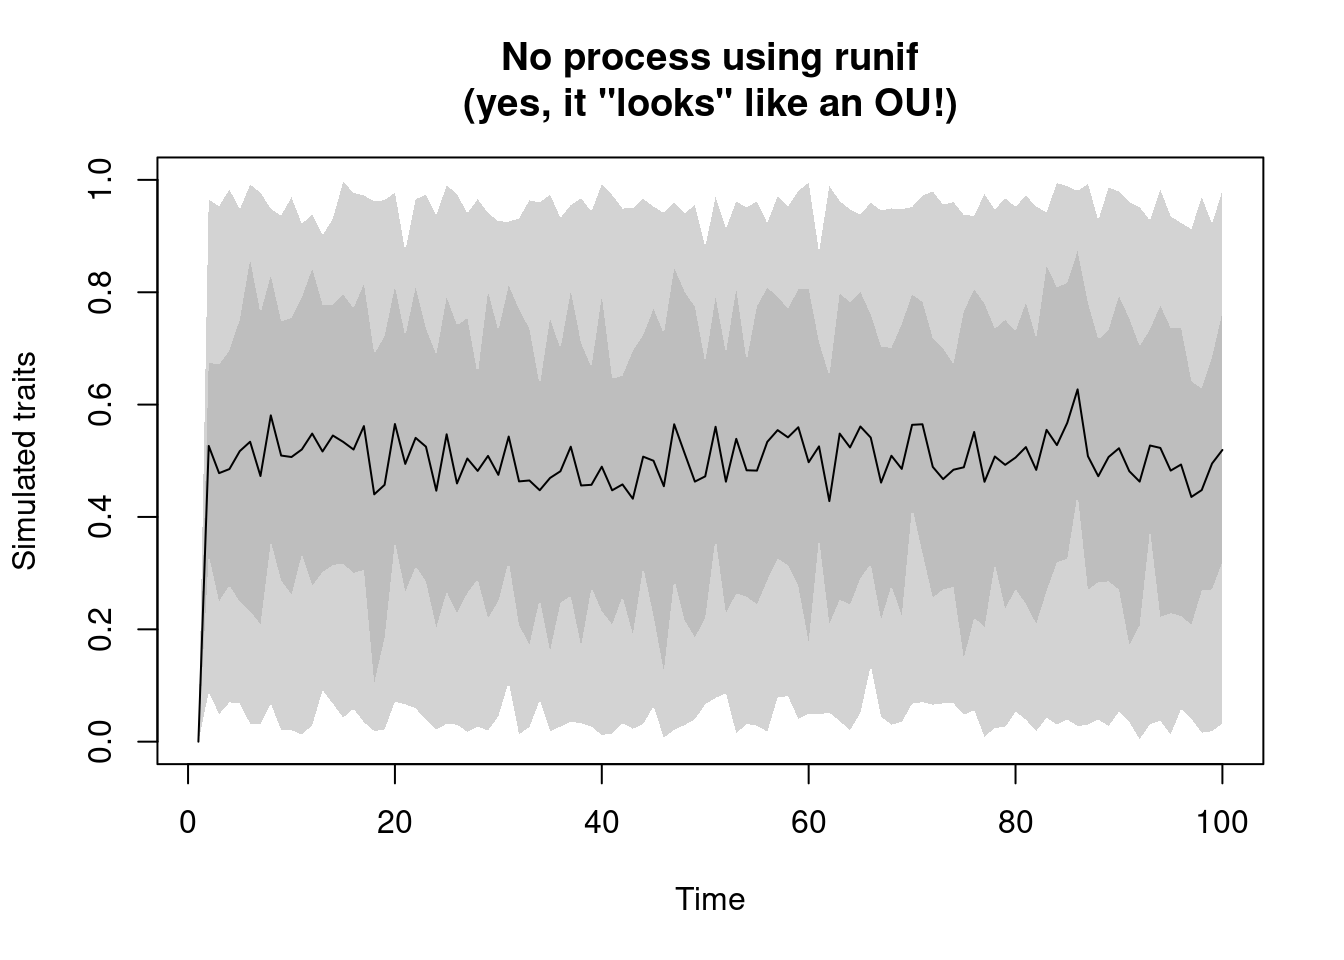
\includegraphics{dads_manual_files/figure-latex/unnamed-chunk-45-1.pdf}

It is of course to use more complex branch length modifiers that intakes different conditions and specific modification rather than simply always output a value of one.

\hypertarget{allowarguments}{%
\subsection{The allowed arguments}\label{allowarguments}}

It is of course possible to design some more advanced function to interact with the birth death process.
You can create a function for \texttt{branch.length}, \texttt{selection} and \texttt{speciation} that involve any of the following arguments:

\begin{itemize}
\tightlist
\item
  \texttt{bd.params}: a named list containing \texttt{"numeric"} values that contains the birth death parameters (at least \texttt{"speciation"} and \texttt{"extinction"});
\item
  \texttt{lineage}: a named list containing the lineage data (see below).
\item
  \texttt{trait.values}: a \texttt{"matrix"} containing \texttt{"numeric"} values with the trait names as column names and the lineages ID as row numbers (you can use it with the function \texttt{parent.traits} to access the trait of the previous node for example).
\item
  \texttt{modify.fun}: a \texttt{"list"} of named \texttt{"function"} (usually passed through \texttt{condition} and \texttt{modify}).
\end{itemize}

The \texttt{lineage} list contains the following elements (missing elements are allowed):

\begin{itemize}
\tightlist
\item
  \texttt{lineage\$parents}: an \texttt{"integer"} vector: the list of parent lineages;
\item
  \texttt{lineage\$livings}: an \texttt{"integer"} vector: the list of lineages still not extinct;
\item
  \texttt{lineage\$drawn}: a single \texttt{"integer"}: the ID of the selected lineage;
\item
  \texttt{lineage\$current}: a single \texttt{"integer"}: the selected lineage (is equal to \texttt{lineage\$livings{[}lineage\$drawn{]}});
\item
  \texttt{lineage\$n}: a single \texttt{"integer"}: the current number of non extinct lineage (is equal to \texttt{length(lineage\$livings))};
\item
  \texttt{lineage\$split}: a \texttt{"logical"} vector: the list of splits for each lineage (\texttt{TRUE}), the number of total tips is equal to \texttt{sum(!lineage\$split)}.
\end{itemize}

In general, unless you know what you're doing, you can ignore most arguments for specific modifiers since they are handled automatically within the \texttt{dads} function.
Therefore any argument can be left undeclared or missing and is always handled internally. For example, if you did not declare \texttt{n.taxa} as a function argument but are using \texttt{n.taxa} in the function, \texttt{n.taxa} will be detected and treated as a current argument automatically as set accordingly within the birth death process (e.g. \texttt{n.taxa} will be set to the current number of taxa every iteration of the process).

For example, we can create a function that increases branch length proportional to the number of species ``alive'' at each time of the simulation in a discrete way. I.e. for discrete numbers of taxa, the branch length increases by jumps (ten fold):

\begin{Shaded}
\begin{Highlighting}[]
\CommentTok{## A more complex binned.branch.length function}
\NormalTok{increasing.brlen <-}\StringTok{ }\ControlFlowTok{function}\NormalTok{(bd.params, lineage) \{}

    \CommentTok{## Setting the cumulated birth and death}
\NormalTok{    birth_death <-}\StringTok{ }\NormalTok{bd.params}\OperatorTok{$}\NormalTok{speciation }\OperatorTok{+}\StringTok{ }\NormalTok{bd.params}\OperatorTok{$}\NormalTok{extinction}

    \CommentTok{## Returning branch lengths depending on different number of taxa}
    \ControlFlowTok{if}\NormalTok{(lineage}\OperatorTok{$}\NormalTok{n }\OperatorTok{<=}\StringTok{ }\DecValTok{5}\NormalTok{) \{}
        \KeywordTok{return}\NormalTok{(}\DecValTok{1}    \OperatorTok{*}\StringTok{ }\KeywordTok{rexp}\NormalTok{(}\DecValTok{1}\NormalTok{, }\KeywordTok{sum}\NormalTok{(}\DecValTok{5} \OperatorTok{*}\StringTok{ }\NormalTok{birth_death)))}
\NormalTok{    \}}
    \ControlFlowTok{if}\NormalTok{(lineage}\OperatorTok{$}\NormalTok{n }\OperatorTok{<=}\StringTok{ }\DecValTok{10}\NormalTok{) \{}
        \KeywordTok{return}\NormalTok{(}\DecValTok{10}   \OperatorTok{*}\StringTok{ }\KeywordTok{rexp}\NormalTok{(}\DecValTok{1}\NormalTok{, }\KeywordTok{sum}\NormalTok{(}\DecValTok{10} \OperatorTok{*}\StringTok{ }\NormalTok{birth_death)))   }
\NormalTok{    \}}
    \ControlFlowTok{if}\NormalTok{(lineage}\OperatorTok{$}\NormalTok{n }\OperatorTok{<=}\StringTok{ }\DecValTok{15}\NormalTok{) \{}
        \KeywordTok{return}\NormalTok{(}\DecValTok{100}  \OperatorTok{*}\StringTok{ }\KeywordTok{rexp}\NormalTok{(}\DecValTok{1}\NormalTok{, }\KeywordTok{sum}\NormalTok{(}\DecValTok{15} \OperatorTok{*}\StringTok{ }\NormalTok{birth_death)))      }
\NormalTok{    \}}
    \ControlFlowTok{if}\NormalTok{(lineage}\OperatorTok{$}\NormalTok{n }\OperatorTok{<=}\StringTok{ }\DecValTok{20}\NormalTok{) \{}
        \KeywordTok{return}\NormalTok{(}\DecValTok{1000} \OperatorTok{*}\StringTok{ }\KeywordTok{rexp}\NormalTok{(}\DecValTok{1}\NormalTok{, }\KeywordTok{sum}\NormalTok{(}\DecValTok{20} \OperatorTok{*}\StringTok{ }\NormalTok{birth_death)))}
\NormalTok{    \} }\ControlFlowTok{else}\NormalTok{ \{}
        \KeywordTok{return}\NormalTok{(}\DecValTok{1000} \OperatorTok{*}\StringTok{ }\KeywordTok{rexp}\NormalTok{(}\DecValTok{1}\NormalTok{, }\KeywordTok{sum}\NormalTok{(lineage}\OperatorTok{$}\NormalTok{n }\OperatorTok{*}\StringTok{ }\NormalTok{birth_death)))}
\NormalTok{    \}}
\NormalTok{\}}
\end{Highlighting}
\end{Shaded}

We can then create it as a \texttt{"modifiers"} object and run a new simulation:

\begin{Shaded}
\begin{Highlighting}[]
\CommentTok{## Creating a modifiers}
\NormalTok{increasing_modifier <-}\StringTok{ }\KeywordTok{make.modifiers}\NormalTok{(}\DataTypeTok{branch.length =}\NormalTok{ increasing.brlen)}

\CommentTok{## Generating a new tree with this modifier}
\KeywordTok{set.seed}\NormalTok{(}\DecValTok{0}\NormalTok{)}
\NormalTok{increasing_tree <-}\StringTok{ }\KeywordTok{dads}\NormalTok{(}\DataTypeTok{bd.params =}\NormalTok{ bd_params,}
                        \DataTypeTok{stop.rule =}\NormalTok{ stop_rule,}
                        \DataTypeTok{modifiers =}\NormalTok{ increasing_modifier)}
\end{Highlighting}
\end{Shaded}

And we can visualise the difference between the resulting trees:

\begin{Shaded}
\begin{Highlighting}[]
\KeywordTok{par}\NormalTok{(}\DataTypeTok{mfrow =} \KeywordTok{c}\NormalTok{(}\DecValTok{1}\NormalTok{,}\DecValTok{3}\NormalTok{))}
\KeywordTok{plot}\NormalTok{(default_tree,    }\DataTypeTok{main =} \StringTok{"Default modifier"}\NormalTok{)}
\KeywordTok{plot}\NormalTok{(modified_tree,   }\DataTypeTok{main =} \StringTok{"Constant branch length}\CharTok{\textbackslash{}n}\StringTok{modifier"}\NormalTok{)}
\KeywordTok{plot}\NormalTok{(increasing_tree, }\DataTypeTok{main =} \StringTok{"Increasing branch length}\CharTok{\textbackslash{}n}\StringTok{modifier (binned)"}\NormalTok{)}
\end{Highlighting}
\end{Shaded}

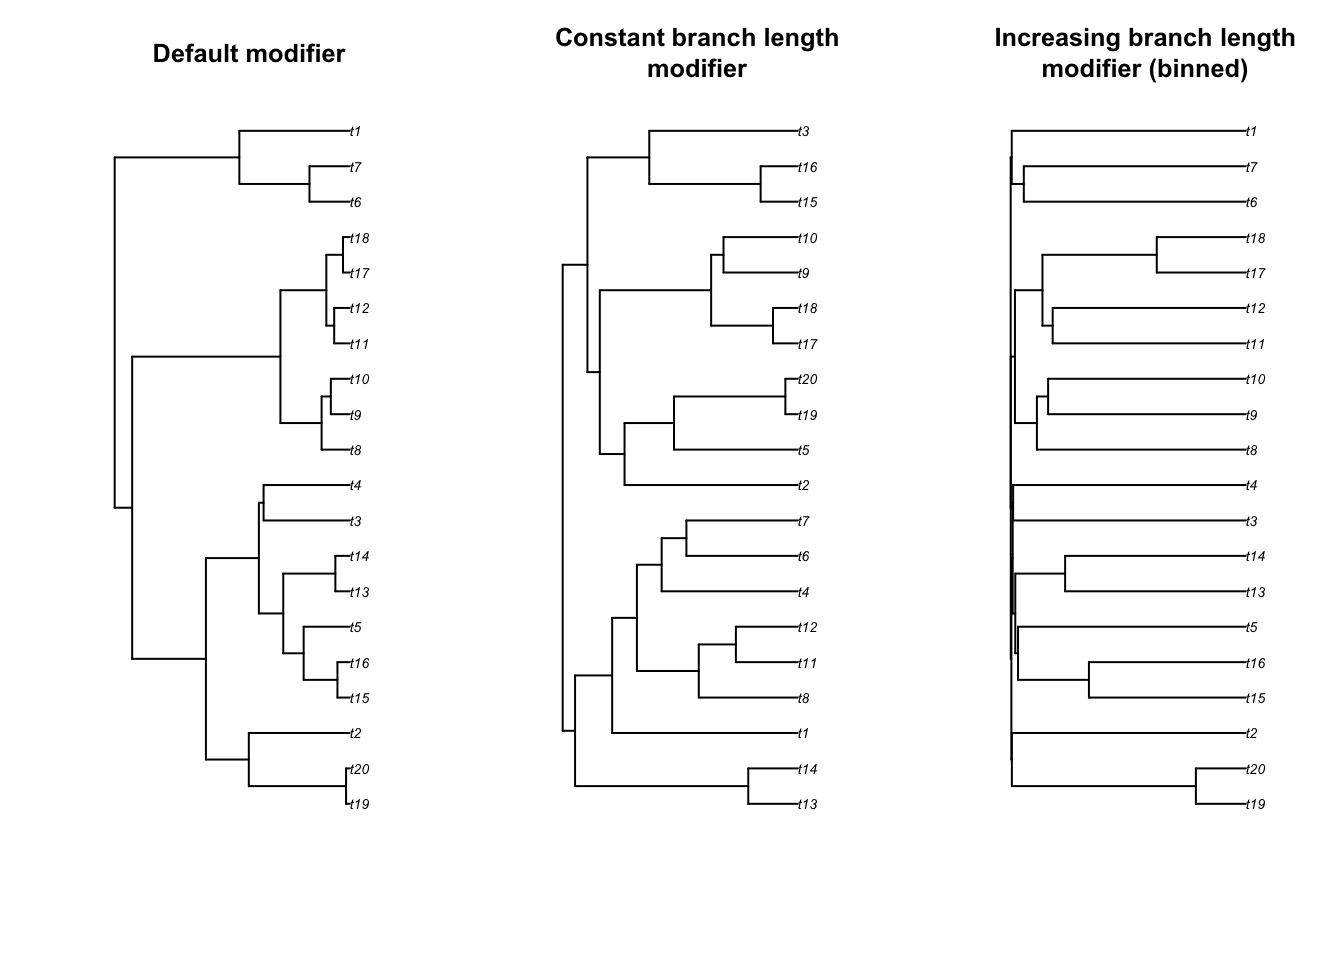
\includegraphics{dads_manual_files/figure-latex/unnamed-chunk-48-1.pdf}

\hypertarget{the-selection-function-selection}{%
\section{\texorpdfstring{The selection function (\texttt{selection})}{The selection function (selection)}}\label{the-selection-function-selection}}

The \texttt{selection} function is used in the birth death process to know which lineage to select when running a speciation (or extinction!) event.
By default, this function randomly selects one taxon that is currently not extinct (using: \texttt{sample(1:n.taxa,\ 1))}.
Similarly as \texttt{branch.length} it is possible to modify this part of the birth death process.
For example, we could simply select always the last created lineage (to create a ``ladder'' or most asymmetric tree):

\begin{Shaded}
\begin{Highlighting}[]
\CommentTok{## Our function to always select the last taxon}
\CommentTok{## (making sure it returns an integer)}
\NormalTok{select.last <-}\StringTok{ }\ControlFlowTok{function}\NormalTok{(lineage) \{}
    \KeywordTok{return}\NormalTok{(}\KeywordTok{as.integer}\NormalTok{(lineage}\OperatorTok{$}\NormalTok{n))}
\NormalTok{\}}
\end{Highlighting}
\end{Shaded}

\begin{quote}
Note that here the function can only intake the \protect\hyperlink{allowarguments}{allowed arguments as described above} (here \texttt{n.taxa}: the number of current living taxa).
\end{quote}

We can then create a \texttt{"modifiers"} object the same way as before using this time the \texttt{selection} argument:

\begin{Shaded}
\begin{Highlighting}[]
\CommentTok{## A modifier for selection}
\NormalTok{ladderised_modifier <-}\StringTok{ }\KeywordTok{make.modifiers}\NormalTok{(}\DataTypeTok{selection =}\NormalTok{ select.last)}
\CommentTok{## Generating a new tree with this modifier}
\KeywordTok{set.seed}\NormalTok{(}\DecValTok{0}\NormalTok{)}
\NormalTok{ladderised_tree <-}\StringTok{ }\KeywordTok{dads}\NormalTok{(}\DataTypeTok{bd.params =}\NormalTok{ bd_params,}
                        \DataTypeTok{stop.rule =}\NormalTok{ stop_rule,}
                        \DataTypeTok{modifiers =}\NormalTok{ ladderised_modifier)}
\CommentTok{## Displaying the results}
\KeywordTok{par}\NormalTok{(}\DataTypeTok{mfrow =} \KeywordTok{c}\NormalTok{(}\DecValTok{1}\NormalTok{,}\DecValTok{2}\NormalTok{))}
\KeywordTok{plot}\NormalTok{(default_tree,    }\DataTypeTok{main =} \StringTok{"Default modifier"}\NormalTok{)}
\KeywordTok{plot}\NormalTok{(ladderised_tree, }\DataTypeTok{main =} \StringTok{"Ladderising modifier"}\NormalTok{)}
\end{Highlighting}
\end{Shaded}

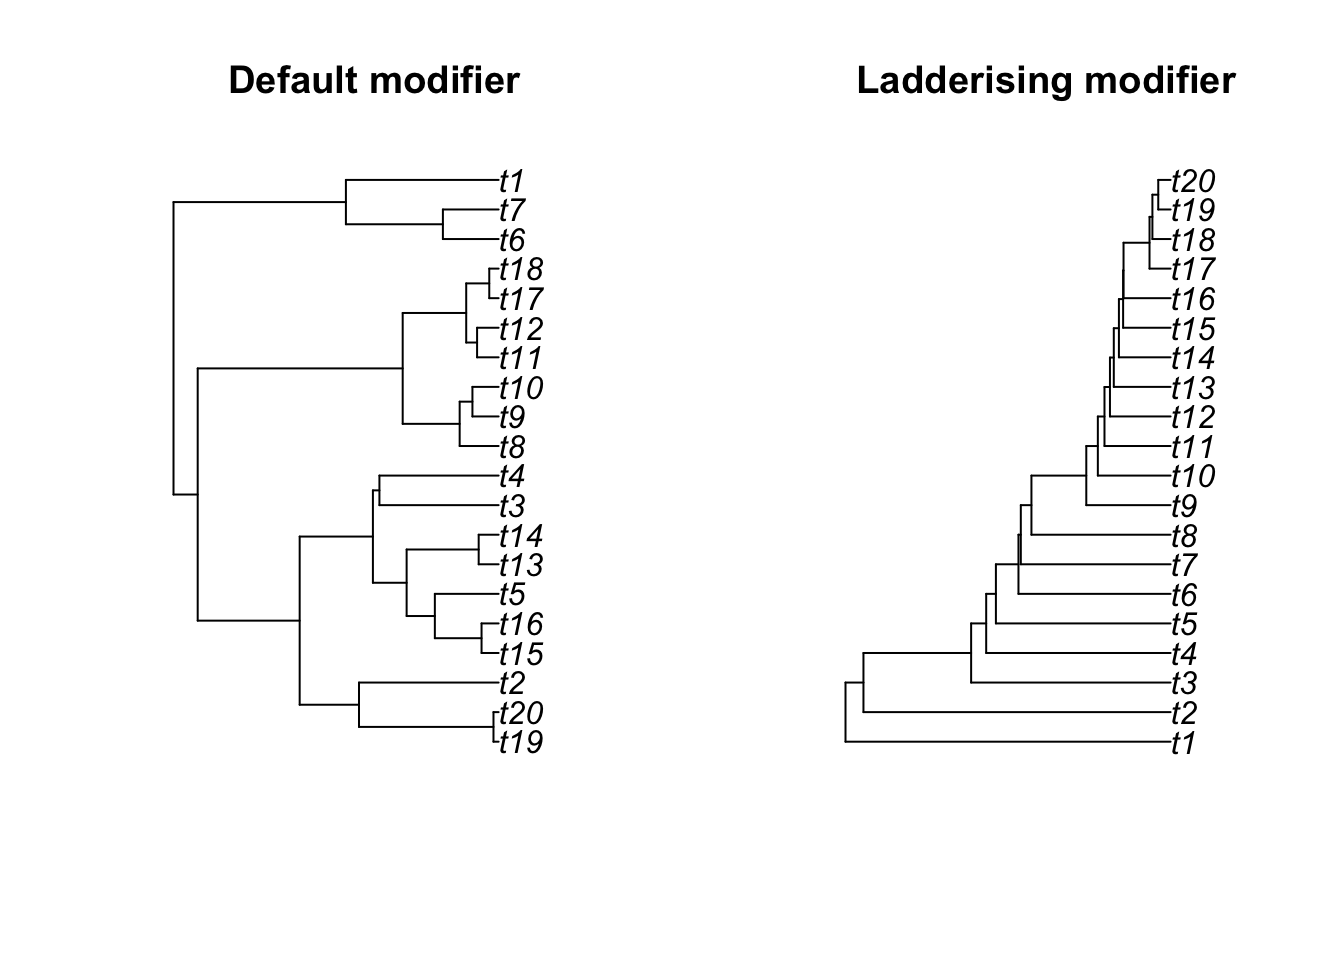
\includegraphics{dads_manual_files/figure-latex/unnamed-chunk-50-1.pdf}

Again, it is of course possible to make the modifier more complex and in combination with other elements of the tree.
For example, we can create a \texttt{"dads"} object that also creates a trait a add to it a \texttt{selection} modifier that only selects for tips with positive trait values.

\begin{Shaded}
\begin{Highlighting}[]
\CommentTok{## Our function that only select taxa with positive trait values}
\NormalTok{select.positive <-}\StringTok{ }\ControlFlowTok{function}\NormalTok{(trait.values, lineage) \{}
    \CommentTok{## Selecting the taxa with positive traits only}
\NormalTok{    positives <-}\StringTok{ }\KeywordTok{as.integer}\NormalTok{(}\KeywordTok{rownames}\NormalTok{(trait.values)[}\KeywordTok{which}\NormalTok{(trait.values[, }\DecValTok{1}\NormalTok{] }\OperatorTok{>=}\StringTok{ }\DecValTok{0}\NormalTok{)])}

    \CommentTok{## Select the current taxa that descend from a node with a positive value}
\NormalTok{    positive_living <-}\StringTok{ }\KeywordTok{cbind}\NormalTok{(lineage}\OperatorTok{$}\NormalTok{parents, }\KeywordTok{seq_along}\NormalTok{(lineage}\OperatorTok{$}\NormalTok{split)}
\NormalTok{                             )[}\KeywordTok{which}\NormalTok{(lineage}\OperatorTok{$}\NormalTok{parents }\OperatorTok\StringTok{ }\NormalTok{positives), }\DecValTok{2}\NormalTok{]}

    \CommentTok{## Select one tip randomly in the ones with descendants with positive values}
    \KeywordTok{return}\NormalTok{(}\KeywordTok{sample}\NormalTok{(}\KeywordTok{which}\NormalTok{(lineage}\OperatorTok{$}\NormalTok{livings }\OperatorTok\StringTok{ }\NormalTok{positive_living), }\DecValTok{1}\NormalTok{))}
\NormalTok{\}}

\CommentTok{## Creating the modifier}
\NormalTok{positive_skew <-}\StringTok{ }\KeywordTok{make.modifiers}\NormalTok{(}\DataTypeTok{selection =}\NormalTok{ select.positive)}

\CommentTok{## Creating a (default) trait object}
\NormalTok{BM_trait <-}\StringTok{ }\KeywordTok{make.traits}\NormalTok{()}

\CommentTok{## Simulate a tree and trait with no modifier}
\KeywordTok{set.seed}\NormalTok{(}\DecValTok{1}\NormalTok{)}
\NormalTok{default_dads <-}\StringTok{ }\KeywordTok{dads}\NormalTok{(}\DataTypeTok{bd.params =}\NormalTok{ bd_params,}
                     \DataTypeTok{stop.rule =}\NormalTok{ stop_rule,}
                     \DataTypeTok{traits    =}\NormalTok{ BM_trait)}

\CommentTok{## Simulate a tree and trait with the modifier}
\KeywordTok{set.seed}\NormalTok{(}\DecValTok{1}\NormalTok{)}
\NormalTok{skewed_trait_dads <-}\StringTok{ }\KeywordTok{dads}\NormalTok{(}\DataTypeTok{bd.params =}\NormalTok{ bd_params,}
                          \DataTypeTok{stop.rule =}\NormalTok{ stop_rule,}
                          \DataTypeTok{traits    =}\NormalTok{ BM_trait,}
                          \DataTypeTok{modifiers =}\NormalTok{ positive_skew)}

\CommentTok{## Plotting the differences in trees and traits}
\KeywordTok{par}\NormalTok{(}\DataTypeTok{mfrow =} \KeywordTok{c}\NormalTok{(}\DecValTok{1}\NormalTok{, }\DecValTok{2}\NormalTok{))}
\KeywordTok{plot}\NormalTok{(default_dads, }\DataTypeTok{main =} \StringTok{"Default trait and tree"}\NormalTok{)}
\KeywordTok{plot}\NormalTok{(skewed_trait_dads, }\DataTypeTok{main =} \StringTok{"Skewed trait and tree"}\NormalTok{)}
\end{Highlighting}
\end{Shaded}

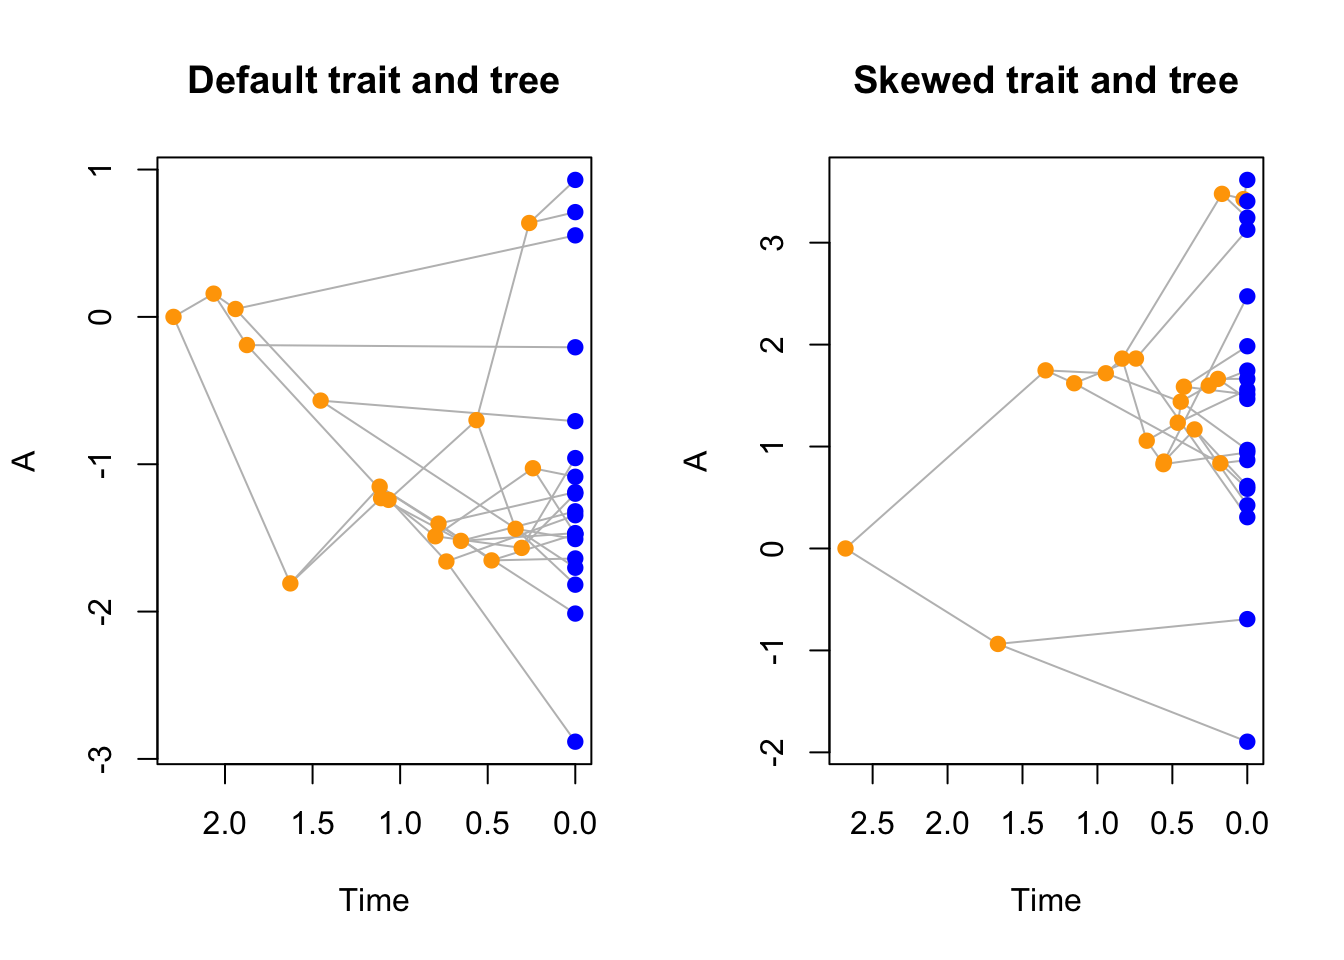
\includegraphics{dads_manual_files/figure-latex/unnamed-chunk-51-1.pdf}

\hypertarget{the-speciation-function-speciation}{%
\section{\texorpdfstring{The speciation function (\texttt{speciation})}{The speciation function (speciation)}}\label{the-speciation-function-speciation}}

The third function that can be used to modify the birth death process is the \texttt{speciation} function.
This one is used during the birth death process to decide whether a lineages speciates (creating a node and two new lineages) or goes extinct (creating a tip).

\begin{quote}
Note that the \texttt{speciation} function only affects tips or nodes before the simulation reaches the \texttt{stop.rule}.
The then surviving lineages are all automatically transformed into tips.
\end{quote}

By default, the \texttt{speciation} function is trigger a speciation even if a number randomly drawn from a uniform distribution is lower than the ratio between the speciation and the speciation and extinction parameter. If the randomly drawn number is higher, the lineage goes extinct.

\begin{Shaded}
\begin{Highlighting}[]
\CommentTok{## The speciation in pseudo-code:}
\KeywordTok{runif}\NormalTok{(}\DecValTok{1}\NormalTok{) }\OperatorTok{<}\StringTok{ }\NormalTok{speciation}\OperatorTok{/}\StringTok{ }\NormalTok{(speciation }\OperatorTok{+}\StringTok{ }\NormalTok{extinction)}
\end{Highlighting}
\end{Shaded}

Creating a \texttt{"modifiers"} with a \texttt{speciation} function works the same way as for \texttt{branch.length} and \texttt{selection} but the function that will be used needs to output a logical value (see table \protect\hyperlink{summarymodifiers}{below}).
Once the function is created simply input your function for speciation in the modifier and run the \texttt{dads} function with that modifier:

\begin{Shaded}
\begin{Highlighting}[]
\CommentTok{## Speciating or going extinct randomly}
\CommentTok{## (regardless of the extinction parameter)}
\NormalTok{random.extinct  <-}\StringTok{ }\ControlFlowTok{function}\NormalTok{() \{}
    \KeywordTok{return}\NormalTok{(}\KeywordTok{sample}\NormalTok{(}\KeywordTok{c}\NormalTok{(}\OtherTok{TRUE}\NormalTok{, }\OtherTok{FALSE}\NormalTok{), }\DecValTok{1}\NormalTok{))}
\NormalTok{\}}

\CommentTok{## Creating the modifiers object}
\NormalTok{random_extinction <-}\StringTok{ }\KeywordTok{make.modifiers}\NormalTok{(}\DataTypeTok{speciation =}\NormalTok{ random.extinct)}

\CommentTok{## Generating a new tree with this modifier}
\KeywordTok{set.seed}\NormalTok{(}\DecValTok{0}\NormalTok{)}
\NormalTok{modified_tree <-}\StringTok{ }\KeywordTok{dads}\NormalTok{(}\DataTypeTok{bd.params =}\NormalTok{ bd_params,}
                      \DataTypeTok{stop.rule =}\NormalTok{ stop_rule,}
                      \DataTypeTok{modifiers =}\NormalTok{ random_extinction)}

\KeywordTok{par}\NormalTok{(}\DataTypeTok{mfrow =} \KeywordTok{c}\NormalTok{(}\DecValTok{1}\NormalTok{,}\DecValTok{2}\NormalTok{))}
\KeywordTok{plot}\NormalTok{(default_tree,  }\DataTypeTok{main =} \StringTok{"Default modifier"}\NormalTok{)}
\KeywordTok{plot}\NormalTok{(modified_tree, }\DataTypeTok{main =} \StringTok{"Random extinction}\CharTok{\textbackslash{}n}\StringTok{modifier"}\NormalTok{)}
\end{Highlighting}
\end{Shaded}

Note how every lineage end up going extinct!
And again, we can make some more advanced modifiers: for example, one where a tip always goes extinct if their ancestor has a negative trait value (here we will also introduce the utility function \texttt{parent.trait} that automatically selects the trait values of the parent of the current lineage.

\begin{Shaded}
\begin{Highlighting}[]
\CommentTok{## A modifier for removing tips with negative values}
\NormalTok{bias.trait <-}\StringTok{ }\ControlFlowTok{function}\NormalTok{(trait.values, lineage) \{}
    \ControlFlowTok{if}\NormalTok{(}\KeywordTok{parent.traits}\NormalTok{(trait.values, lineage) }\OperatorTok{<}\StringTok{ }\DecValTok{0}\NormalTok{) \{}
        \CommentTok{## Go extinct!}
        \KeywordTok{return}\NormalTok{(}\OtherTok{FALSE}\NormalTok{)}
\NormalTok{    \} }\ControlFlowTok{else}\NormalTok{ \{}
        \CommentTok{## Speciate}
        \KeywordTok{return}\NormalTok{(}\OtherTok{TRUE}\NormalTok{)}
\NormalTok{    \}}
\NormalTok{\}}

\CommentTok{## Creating the modifier}
\NormalTok{biased_trait <-}\StringTok{ }\KeywordTok{make.modifiers}\NormalTok{(}\DataTypeTok{speciation =}\NormalTok{ bias.trait)}

\CommentTok{## Simulate a tree and trait with the modifier}
\KeywordTok{set.seed}\NormalTok{(}\DecValTok{1}\NormalTok{)}
\NormalTok{biased_trait_dads <-}\StringTok{ }\KeywordTok{dads}\NormalTok{(}\DataTypeTok{bd.params =}\NormalTok{ bd_params,}
                          \DataTypeTok{stop.rule =}\NormalTok{ stop_rule,}
                          \DataTypeTok{traits    =}\NormalTok{ BM_trait,}
                          \DataTypeTok{modifiers =}\NormalTok{ biased_trait)}

\CommentTok{## Plotting the differences in trees and traits}
\KeywordTok{par}\NormalTok{(}\DataTypeTok{mfrow =} \KeywordTok{c}\NormalTok{(}\DecValTok{1}\NormalTok{, }\DecValTok{2}\NormalTok{))}
\KeywordTok{plot}\NormalTok{(default_dads, }\DataTypeTok{main =} \StringTok{"Default trait and tree"}\NormalTok{)}
\KeywordTok{plot}\NormalTok{(biased_trait_dads, }\DataTypeTok{main =} \StringTok{"Biased trait and tree"}\NormalTok{)}
\end{Highlighting}
\end{Shaded}

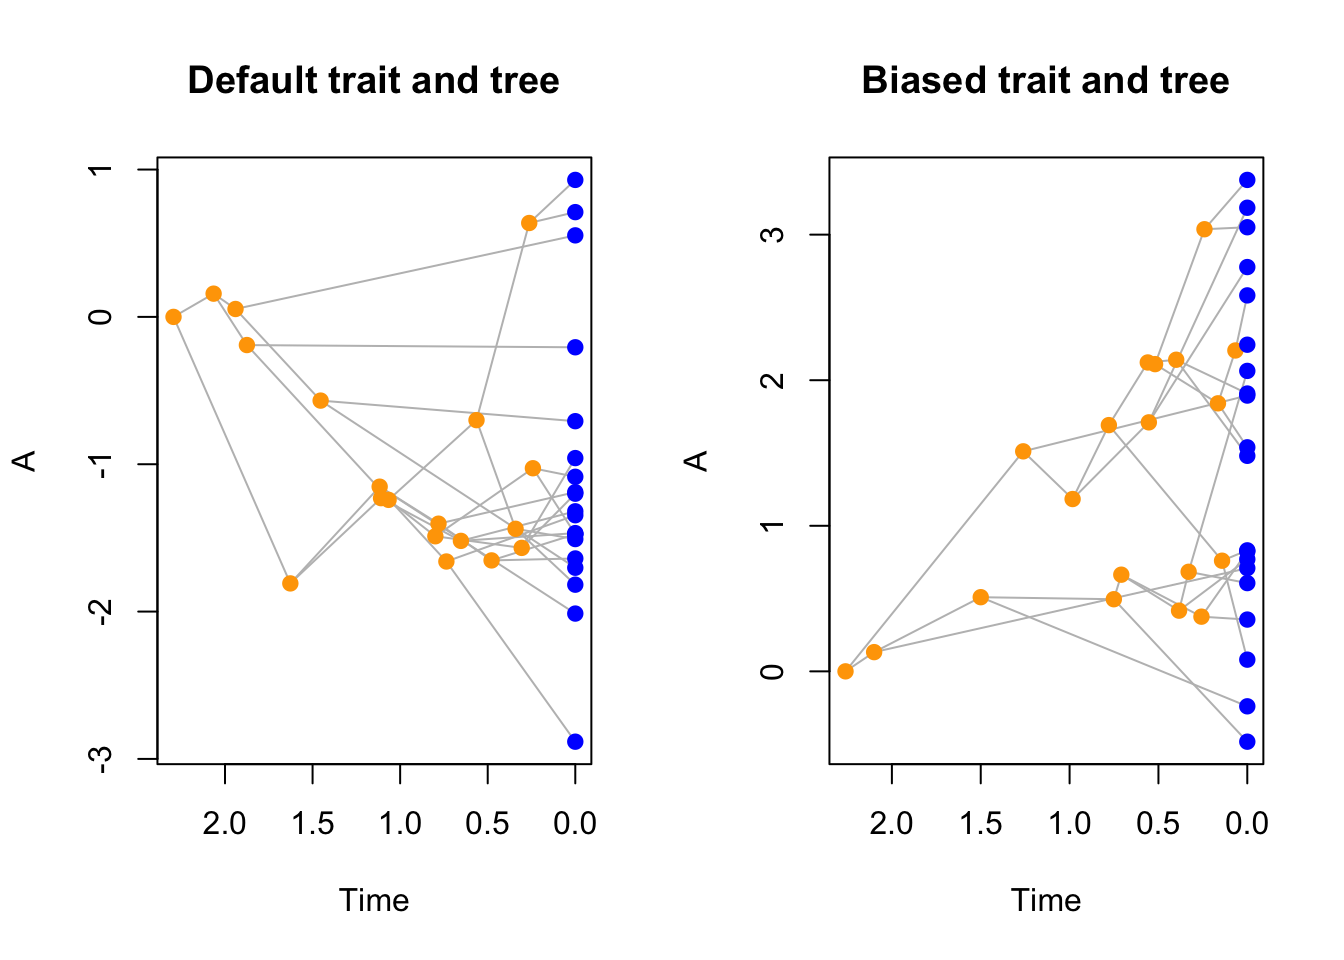
\includegraphics{dads_manual_files/figure-latex/unnamed-chunk-54-1.pdf}

\hypertarget{summarymodifiers}{%
\section{\texorpdfstring{Summary of the inputs and outputs for the \texttt{branch.length}, \texttt{selection} and \texttt{speciation} modifiers}{Summary of the inputs and outputs for the branch.length, selection and speciation modifiers}}\label{summarymodifiers}}

\begin{longtable}[]{@{}lll@{}}
\toprule
modifier name & accepted input (arguments) & required output (class)\tabularnewline
\midrule
\endhead
\texttt{branch.length} & \texttt{bd.params}, \texttt{lineage}, \texttt{trait.values} & \texttt{"numeric"}\tabularnewline
\texttt{selection} & \texttt{bd.params}, \texttt{lineage}, \texttt{trait.values} & \texttt{"integer"}\tabularnewline
\texttt{speciation} & \texttt{bd.params}, \texttt{lineage}, \texttt{trait.values} & \texttt{"logical"}\tabularnewline
\bottomrule
\end{longtable}

\hypertarget{the-condition-and-modify-functions-condition-and-modify}{%
\section{\texorpdfstring{The condition and modify functions (\texttt{condition} and \texttt{modify})}{The condition and modify functions (condition and modify)}}\label{the-condition-and-modify-functions-condition-and-modify}}

In the examples above, we have seen how to specify modifications to the birth death process (via \texttt{branch.length}, \texttt{selection} and \texttt{speciation}), however, one might note that these modifications are not dynamic.
In other words, throughout the process, the modifications remain constant (even if they are conditional).
It is however possible to code the \texttt{"modifiers"} so that they can be affected by \texttt{"events"} objects (see next chapter).

To do so, you can formally declare conditions (\texttt{condition}) and modifications (\texttt{modify}) as internal functions that can then be modified my an \texttt{"events"} object.
\texttt{condition} and \texttt{modify} are hard coded in the \texttt{branch.length} function that they concern, i.e.~they are variables (functions) within the function.

\hypertarget{combining-and-editing-modifiers-add}{%
\section{\texorpdfstring{Combining and editing modifiers (\texttt{add})}{Combining and editing modifiers (add)}}\label{combining-and-editing-modifiers-add}}

\hypertarget{testing-modifiers-test}{%
\section{\texorpdfstring{Testing modifiers (\texttt{test})}{Testing modifiers (test)}}\label{testing-modifiers-test}}

\hypertarget{demo-runnable}{%
\section{Demo runnable}\label{demo-runnable}}

\hypertarget{makeevents}{%
\chapter{\texorpdfstring{Making events with \texttt{make.events()}}{Making events with make.events()}}\label{makeevents}}

\hypertarget{conditions}{%
\section{Conditions}\label{conditions}}

\hypertarget{modifications}{%
\section{Modifications}\label{modifications}}

\hypertarget{some-events-examples}{%
\section{Some events examples}\label{some-events-examples}}

\hypertarget{random-mass-extinction-after-some-time}{%
\subsection{Random mass extinction after some time}\label{random-mass-extinction-after-some-time}}

\begin{Shaded}
\begin{Highlighting}[]
\CommentTok{## Simulation parameters}
\NormalTok{stop.rule <-}\StringTok{ }\KeywordTok{list}\NormalTok{(}\DataTypeTok{max.time =} \DecValTok{5}\NormalTok{)}
\NormalTok{bd.params <-}\StringTok{ }\KeywordTok{list}\NormalTok{(}\DataTypeTok{extinction =} \DecValTok{0}\NormalTok{, }\DataTypeTok{speciation =} \DecValTok{1}\NormalTok{)}

\CommentTok{## 80% mass extinction at time 4}
\NormalTok{mass_extinction <-}\StringTok{ }\KeywordTok{make.events}\NormalTok{(}
                      \DataTypeTok{target =} \StringTok{"taxa"}\NormalTok{,}
                      \DataTypeTok{condition =} \KeywordTok{time.condition}\NormalTok{(}\DecValTok{4}\NormalTok{),}
                      \DataTypeTok{modification =} \KeywordTok{random.extinction}\NormalTok{(}\FloatTok{0.8}\NormalTok{))}

\CommentTok{## Running the simulations}
\KeywordTok{set.seed}\NormalTok{(}\DecValTok{1}\NormalTok{)}
\NormalTok{results <-}\StringTok{ }\KeywordTok{dads}\NormalTok{(}\DataTypeTok{bd.params =}\NormalTok{ bd.params,}
                \DataTypeTok{stop.rule =}\NormalTok{ stop.rule,}
                \DataTypeTok{events    =}\NormalTok{ mass_extinction)}
\CommentTok{## Plotting the results}
\KeywordTok{plot}\NormalTok{(results, }\DataTypeTok{show.tip.label =} \OtherTok{FALSE}\NormalTok{)}
\KeywordTok{axisPhylo}\NormalTok{()}
\end{Highlighting}
\end{Shaded}

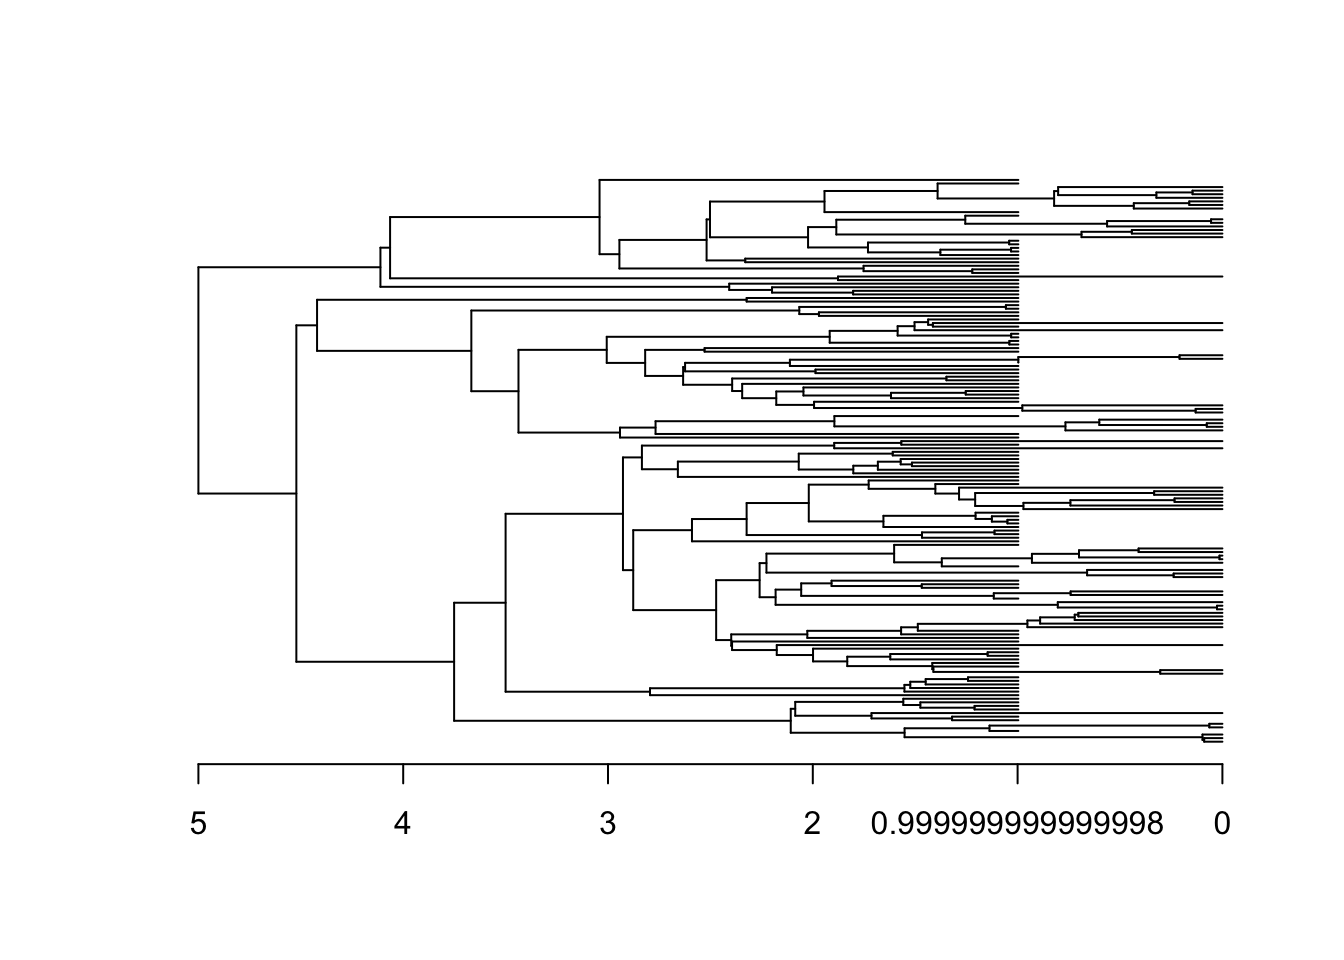
\includegraphics{dads_manual_files/figure-latex/unnamed-chunk-57-1.pdf}

\hypertarget{extinction-based-on-a-trait-value-after-some-time}{%
\subsection{Extinction based on a trait value after some time}\label{extinction-based-on-a-trait-value-after-some-time}}

\begin{Shaded}
\begin{Highlighting}[]
\CommentTok{## Simulation parameters}
\NormalTok{stop.rule <-}\StringTok{ }\KeywordTok{list}\NormalTok{(}\DataTypeTok{max.time =} \DecValTok{5}\NormalTok{)}
\NormalTok{bd.params <-}\StringTok{ }\KeywordTok{list}\NormalTok{(}\DataTypeTok{extinction =} \DecValTok{0}\NormalTok{, }\DataTypeTok{speciation =} \DecValTok{1}\NormalTok{)}

\CommentTok{## Extinction of any tips with trait < 1 at time 4}
\NormalTok{trait_extinction <-}\StringTok{ }\KeywordTok{make.events}\NormalTok{(}
                      \DataTypeTok{target =} \StringTok{"taxa"}\NormalTok{,}
                      \DataTypeTok{condition =} \KeywordTok{time.condition}\NormalTok{(}\DecValTok{4}\NormalTok{),}
                      \DataTypeTok{modification =} \KeywordTok{trait.extinction}\NormalTok{(}\DecValTok{1}\NormalTok{))}

\CommentTok{## Running the simulations}
\KeywordTok{set.seed}\NormalTok{(}\DecValTok{7}\NormalTok{)}
\NormalTok{results <-}\StringTok{ }\KeywordTok{dads}\NormalTok{(}\DataTypeTok{bd.params =}\NormalTok{ bd.params,}
                \DataTypeTok{stop.rule =}\NormalTok{ stop.rule,}
                \DataTypeTok{traits    =} \KeywordTok{make.traits}\NormalTok{(),}
                \DataTypeTok{events    =}\NormalTok{ trait_extinction)}
\CommentTok{## Plotting the results}
\KeywordTok{plot}\NormalTok{(results)}
\end{Highlighting}
\end{Shaded}

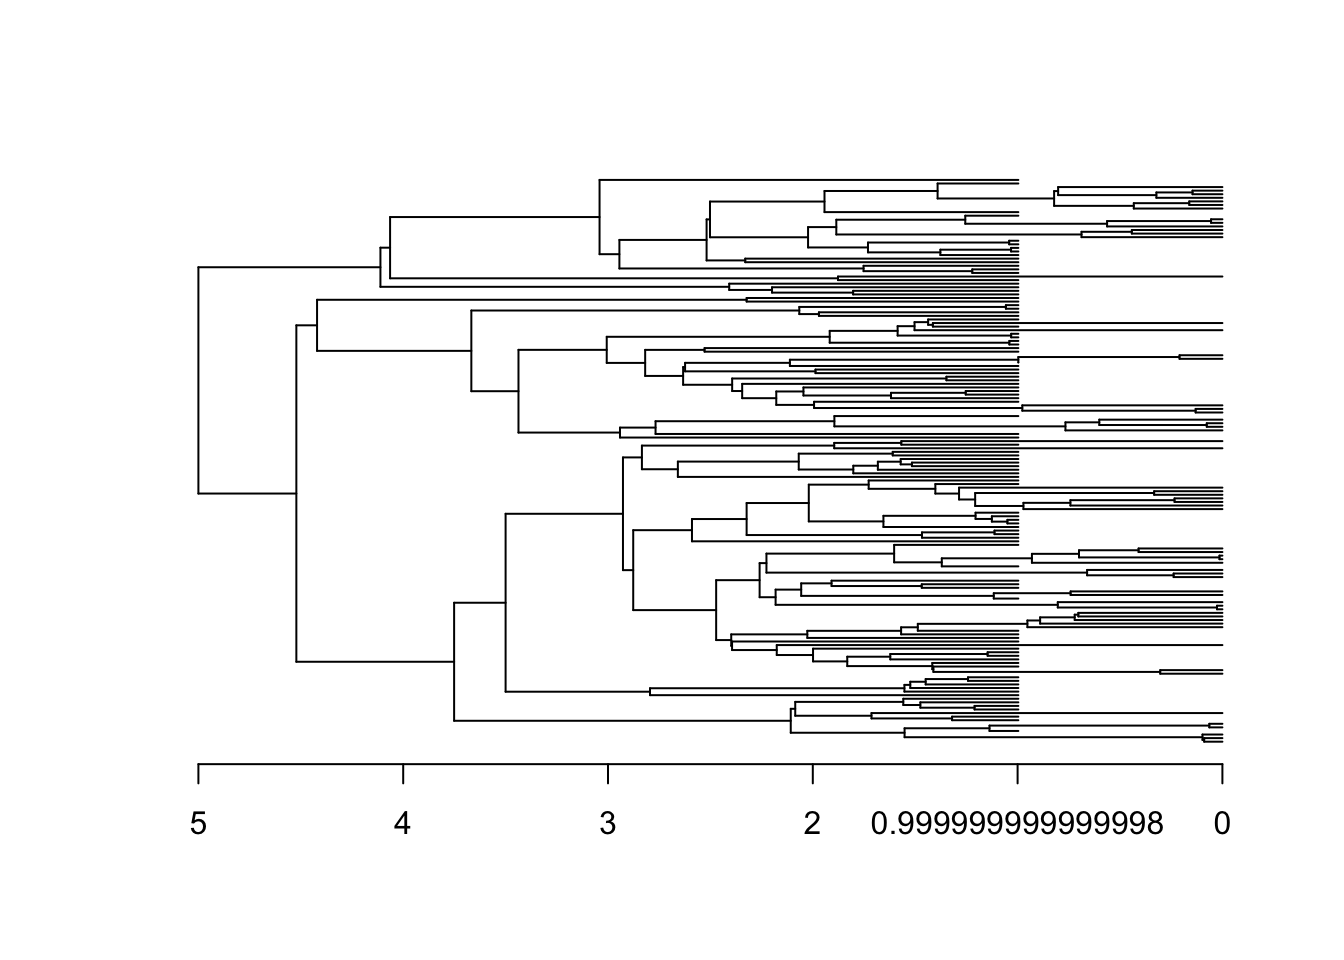
\includegraphics{dads_manual_files/figure-latex/unnamed-chunk-58-1.pdf}

\hypertarget{adding-a-background-extinction-after-reaching-a-number-of-living-taxa}{%
\subsection{Adding a background extinction after reaching a number of living taxa}\label{adding-a-background-extinction-after-reaching-a-number-of-living-taxa}}

\begin{Shaded}
\begin{Highlighting}[]
\CommentTok{## Simulation parameters}
\NormalTok{stop.rule <-}\StringTok{ }\KeywordTok{list}\NormalTok{(}\DataTypeTok{max.living =} \DecValTok{50}\NormalTok{)}
\NormalTok{bd.params <-}\StringTok{ }\KeywordTok{list}\NormalTok{(}\DataTypeTok{extinction =} \DecValTok{0}\NormalTok{, }\DataTypeTok{speciation =} \DecValTok{1}\NormalTok{)}

\CommentTok{## Adding an extinction parameter after 30 taxa}
\NormalTok{background_extinction <-}\StringTok{ }\KeywordTok{make.events}\NormalTok{(}
                      \DataTypeTok{condition    =} \KeywordTok{taxa.condition}\NormalTok{(}\DecValTok{30}\NormalTok{),}
                      \DataTypeTok{target       =} \StringTok{"bd.params"}\NormalTok{,}
                      \DataTypeTok{modification =} \KeywordTok{update.bd.params}\NormalTok{(}\DecValTok{1}\OperatorTok{/}\DecValTok{3}\NormalTok{, }\StringTok{"extinction"}\NormalTok{))}

\CommentTok{## Running the simulations}
\KeywordTok{set.seed}\NormalTok{(}\DecValTok{2}\NormalTok{)}
\NormalTok{results <-}\StringTok{ }\KeywordTok{dads}\NormalTok{(}\DataTypeTok{bd.params =}\NormalTok{ bd.params,}
                \DataTypeTok{stop.rule =}\NormalTok{ stop.rule,}
                \DataTypeTok{events    =}\NormalTok{ background_extinction)}
\CommentTok{## Plotting the results}
\KeywordTok{plot}\NormalTok{(results)}
\end{Highlighting}
\end{Shaded}

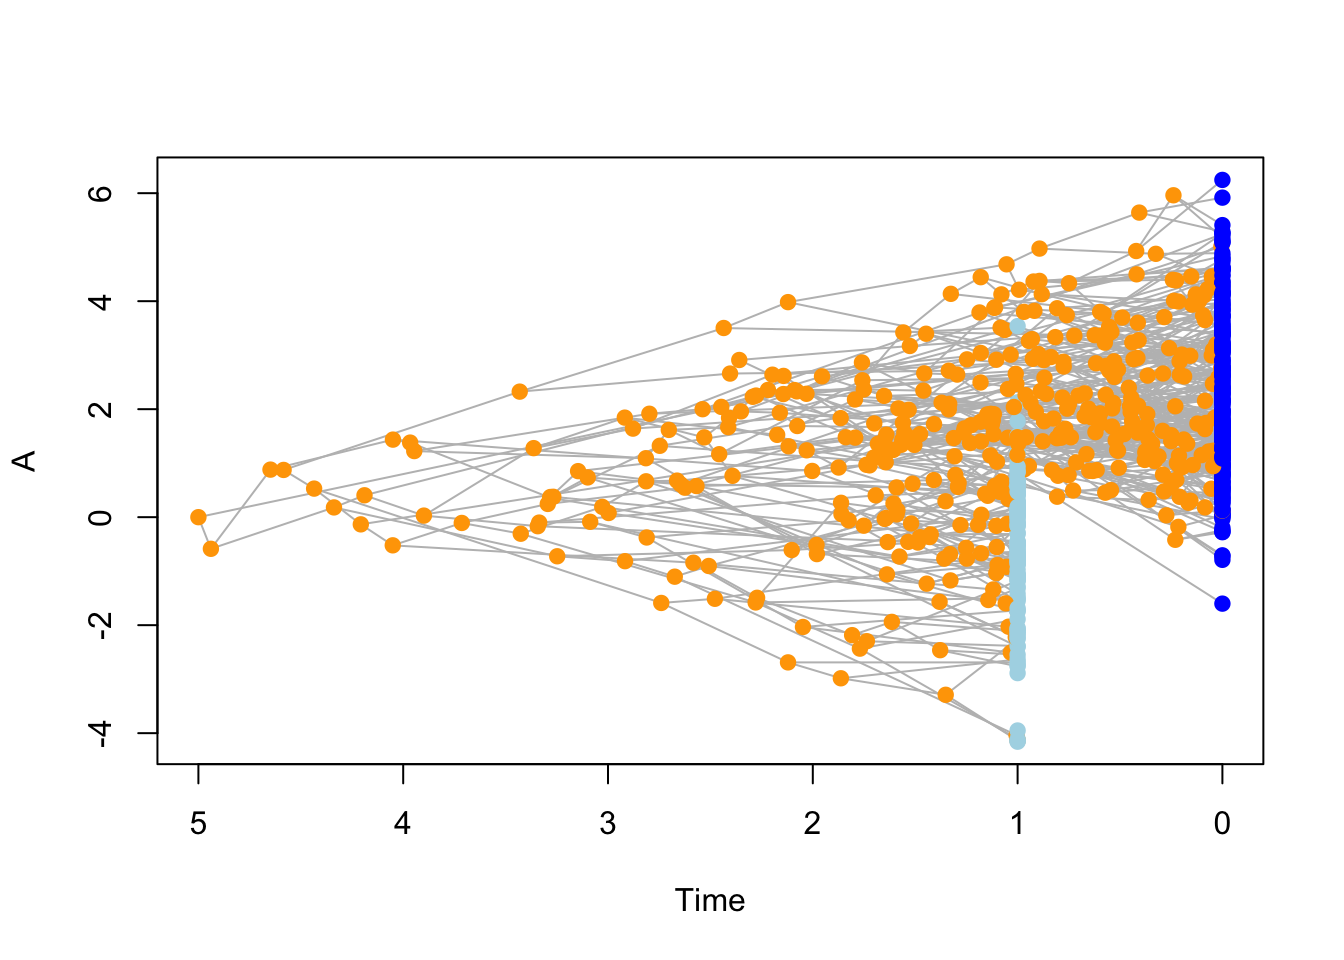
\includegraphics{dads_manual_files/figure-latex/unnamed-chunk-59-1.pdf}

\hypertarget{reducing-speciation-after-some-time}{%
\subsection{Reducing speciation after some time}\label{reducing-speciation-after-some-time}}

\begin{Shaded}
\begin{Highlighting}[]
\CommentTok{## Simulation parameters}
\NormalTok{stop.rule <-}\StringTok{ }\KeywordTok{list}\NormalTok{(}\DataTypeTok{max.time =} \DecValTok{4}\NormalTok{)}
\NormalTok{bd.params <-}\StringTok{ }\KeywordTok{list}\NormalTok{(}\DataTypeTok{extinction =} \DecValTok{0}\NormalTok{, }\DataTypeTok{speciation =} \DecValTok{1}\NormalTok{)}

\CommentTok{## Reducing speciation after reaching time 2}
\NormalTok{reduced_speciation <-}\StringTok{ }\KeywordTok{make.events}\NormalTok{(}
                      \DataTypeTok{condition    =} \KeywordTok{time.condition}\NormalTok{(}\DecValTok{2}\NormalTok{),}
                      \DataTypeTok{target       =} \StringTok{"bd.params"}\NormalTok{,}
                      \DataTypeTok{modification =} \KeywordTok{update.bd.params}\NormalTok{(}\DecValTok{1}\OperatorTok{/}\DecValTok{3}\NormalTok{, }\StringTok{"speciation"}\NormalTok{))}

\KeywordTok{set.seed}\NormalTok{(}\DecValTok{42}\NormalTok{)}
\NormalTok{no_event <-}\StringTok{ }\KeywordTok{dads}\NormalTok{(}\DataTypeTok{bd.params =}\NormalTok{ bd.params,}
                 \DataTypeTok{stop.rule =}\NormalTok{ stop.rule)}
\KeywordTok{set.seed}\NormalTok{(}\DecValTok{42}\NormalTok{)}
\NormalTok{reduced_speciation_event <-}\StringTok{ }\KeywordTok{dads}\NormalTok{(}\DataTypeTok{bd.params =}\NormalTok{ bd.params,}
                                 \DataTypeTok{stop.rule =}\NormalTok{ stop.rule,}
                                 \DataTypeTok{events    =}\NormalTok{ reduced_speciation)}

\CommentTok{## Plot both trees}
\KeywordTok{par}\NormalTok{(}\DataTypeTok{mfrow =} \KeywordTok{c}\NormalTok{(}\DecValTok{1}\NormalTok{, }\DecValTok{2}\NormalTok{))}
\KeywordTok{plot}\NormalTok{(no_event, }\DataTypeTok{main =} \StringTok{"No event"}\NormalTok{)}
\KeywordTok{axisPhylo}\NormalTok{()}
\KeywordTok{plot}\NormalTok{(reduced_speciation_event, }\DataTypeTok{main =} \StringTok{"Reduced speciation after time 2"}\NormalTok{)}
\KeywordTok{axisPhylo}\NormalTok{()}
\end{Highlighting}
\end{Shaded}

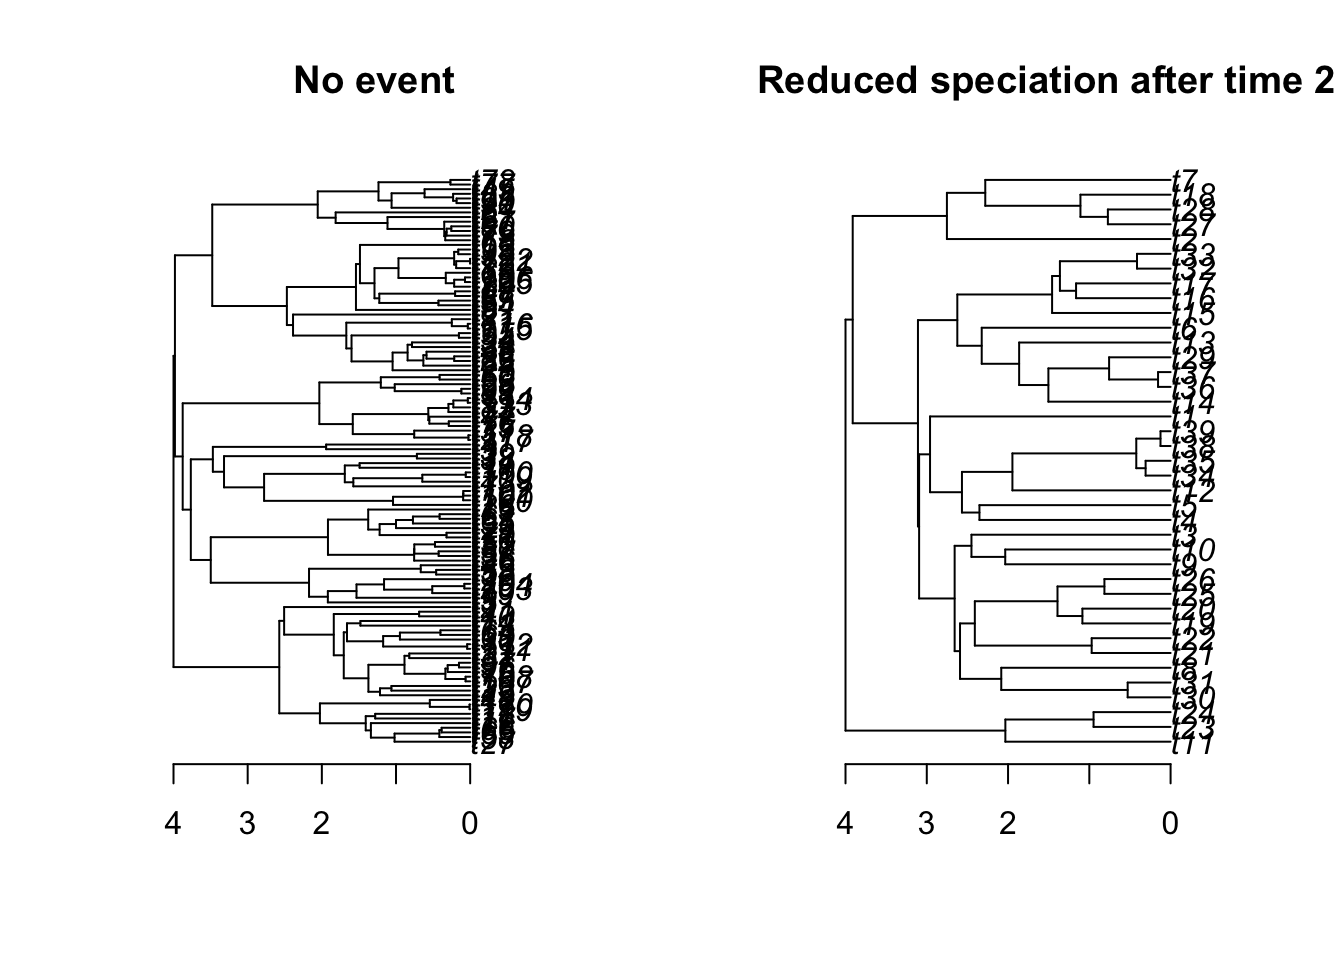
\includegraphics{dads_manual_files/figure-latex/unnamed-chunk-60-1.pdf}

\hypertarget{changing-trait-process-after-some-time}{%
\subsection{Changing trait process after some time}\label{changing-trait-process-after-some-time}}

\begin{Shaded}
\begin{Highlighting}[]
\CommentTok{## Simulation parameters}
\NormalTok{bd.params <-}\StringTok{ }\KeywordTok{list}\NormalTok{(}\DataTypeTok{extinction =} \DecValTok{0}\NormalTok{, }\DataTypeTok{speciation =} \DecValTok{1}\NormalTok{)}
\NormalTok{stop.rule <-}\StringTok{ }\KeywordTok{list}\NormalTok{(}\DataTypeTok{max.time =} \DecValTok{6}\NormalTok{)}
\NormalTok{traits    <-}\StringTok{ }\KeywordTok{make.traits}\NormalTok{()}

\CommentTok{## Create an event to change the trait process}
\NormalTok{change_process <-}\StringTok{ }\KeywordTok{make.events}\NormalTok{(}
                  \DataTypeTok{condition    =} \KeywordTok{time.condition}\NormalTok{(}\DecValTok{5}\NormalTok{),}
                  \DataTypeTok{target       =} \StringTok{"traits"}\NormalTok{,}
                  \DataTypeTok{modification =} \KeywordTok{update.traits}\NormalTok{(}\DataTypeTok{process =}\NormalTok{ OU.process))}

\CommentTok{## Run the simulations}
\KeywordTok{set.seed}\NormalTok{(}\DecValTok{1}\NormalTok{)}
\NormalTok{no_change <-}\StringTok{ }\KeywordTok{dads}\NormalTok{(}\DataTypeTok{bd.params =}\NormalTok{ bd.params,}
                  \DataTypeTok{stop.rule =}\NormalTok{ stop.rule,}
                  \DataTypeTok{traits    =}\NormalTok{ traits)}
\KeywordTok{set.seed}\NormalTok{(}\DecValTok{1}\NormalTok{)}
\NormalTok{process_change <-}\StringTok{ }\KeywordTok{dads}\NormalTok{(}\DataTypeTok{bd.params =}\NormalTok{ bd.params,}
                       \DataTypeTok{stop.rule =}\NormalTok{ stop.rule,}
                       \DataTypeTok{traits    =}\NormalTok{ traits,}
                       \DataTypeTok{events    =}\NormalTok{ change_process)}
\CommentTok{## Plot the results}
\KeywordTok{par}\NormalTok{(}\DataTypeTok{mfrow =} \KeywordTok{c}\NormalTok{(}\DecValTok{1}\NormalTok{,}\DecValTok{2}\NormalTok{))}
\KeywordTok{plot}\NormalTok{(no_change, }\DataTypeTok{ylim =} \KeywordTok{c}\NormalTok{(}\OperatorTok{-}\DecValTok{7}\NormalTok{, }\DecValTok{7}\NormalTok{))}
\KeywordTok{plot}\NormalTok{(process_change, }\DataTypeTok{ylim =} \KeywordTok{c}\NormalTok{(}\OperatorTok{-}\DecValTok{7}\NormalTok{, }\DecValTok{7}\NormalTok{))}
\end{Highlighting}
\end{Shaded}

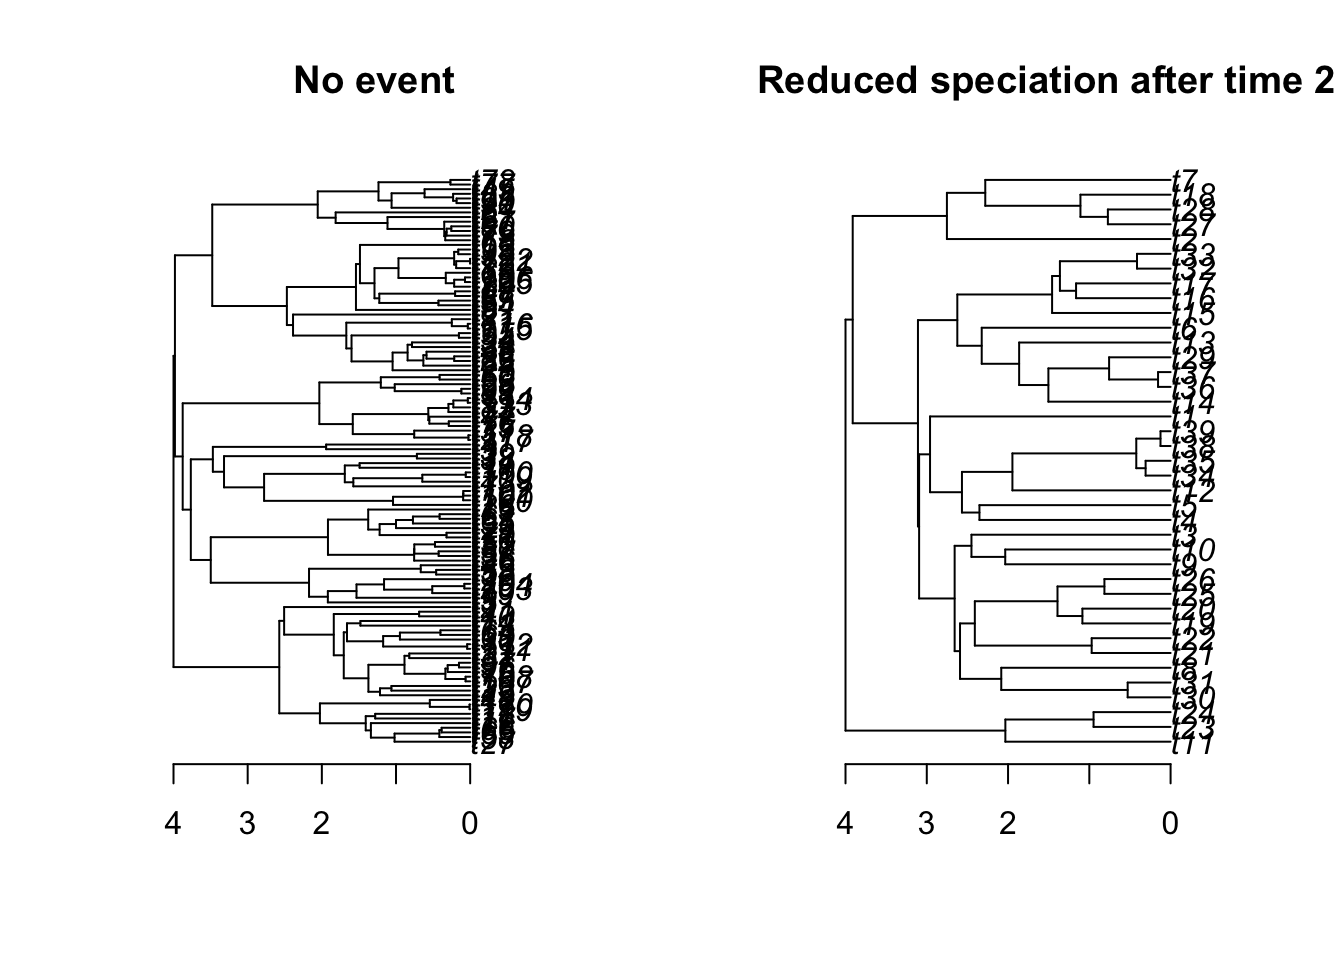
\includegraphics{dads_manual_files/figure-latex/unnamed-chunk-61-1.pdf}

\hypertarget{changing-trait-correlation-after-reaching-a-trait-value}{%
\subsection{Changing trait correlation after reaching a trait value}\label{changing-trait-correlation-after-reaching-a-trait-value}}

\begin{Shaded}
\begin{Highlighting}[]
\CommentTok{## Set the parameters}
\NormalTok{stop.rule <-}\StringTok{ }\KeywordTok{list}\NormalTok{(}\DataTypeTok{max.taxa =} \DecValTok{100}\NormalTok{)}
\NormalTok{bd.params <-}\StringTok{ }\KeywordTok{list}\NormalTok{(}\DataTypeTok{extinction =} \DecValTok{0}\NormalTok{, }\DataTypeTok{speciation =} \DecValTok{1}\NormalTok{)}

\CommentTok{## A correlated trait}
\NormalTok{traits <-}\StringTok{ }\KeywordTok{make.traits}\NormalTok{(}\DataTypeTok{n =} \DecValTok{2}\NormalTok{, }\DataTypeTok{process.args =} \KeywordTok{list}\NormalTok{(}\DataTypeTok{Sigma =} \KeywordTok{matrix}\NormalTok{(}\DecValTok{1}\NormalTok{, }\DecValTok{2}\NormalTok{, }\DecValTok{2}\NormalTok{)))}

\CommentTok{## Event changing a trait correlation}
\NormalTok{change_correlation <-}\StringTok{ }\KeywordTok{make.events}\NormalTok{(}
    \DataTypeTok{condition    =} \KeywordTok{trait.condition}\NormalTok{(}\DecValTok{3}\NormalTok{, }\DataTypeTok{absolute =} \OtherTok{TRUE}\NormalTok{),}
    \DataTypeTok{target       =} \StringTok{"traits"}\NormalTok{,}
    \DataTypeTok{modification =} \KeywordTok{update.traits}\NormalTok{(}\DataTypeTok{process.args =} \KeywordTok{list}\NormalTok{(}\DataTypeTok{Sigma =} \KeywordTok{matrix}\NormalTok{(}\KeywordTok{c}\NormalTok{(}\DecValTok{10}\NormalTok{,}\DecValTok{3}\NormalTok{,}\DecValTok{3}\NormalTok{,}\DecValTok{2}\NormalTok{),}\DecValTok{2}\NormalTok{,}\DecValTok{2}\NormalTok{))))}

\CommentTok{## Run the simulations}
\KeywordTok{set.seed}\NormalTok{(}\DecValTok{8}\NormalTok{)}
\NormalTok{no_event <-}\StringTok{ }\KeywordTok{dads}\NormalTok{(}\DataTypeTok{bd.params =}\NormalTok{ bd.params,}
                 \DataTypeTok{stop.rule =}\NormalTok{ stop.rule,}
                 \DataTypeTok{traits    =}\NormalTok{ traits)}
\KeywordTok{set.seed}\NormalTok{(}\DecValTok{8}\NormalTok{)}
\NormalTok{change_correlation <-}\StringTok{ }\KeywordTok{dads}\NormalTok{(}\DataTypeTok{bd.params =}\NormalTok{ bd.params,}
                           \DataTypeTok{stop.rule =}\NormalTok{ stop.rule,}
                           \DataTypeTok{traits    =}\NormalTok{ traits,}
                           \DataTypeTok{events    =}\NormalTok{ change_correlation)}
\CommentTok{## Visual testing}
\KeywordTok{par}\NormalTok{(}\DataTypeTok{mfrow =} \KeywordTok{c}\NormalTok{(}\DecValTok{1}\NormalTok{,}\DecValTok{2}\NormalTok{))}
\KeywordTok{plot}\NormalTok{(no_event, }\DataTypeTok{trait =} \DecValTok{2}\NormalTok{)}
\KeywordTok{plot}\NormalTok{(change_correlation, }\DataTypeTok{trait =} \DecValTok{2}\NormalTok{)}
\end{Highlighting}
\end{Shaded}

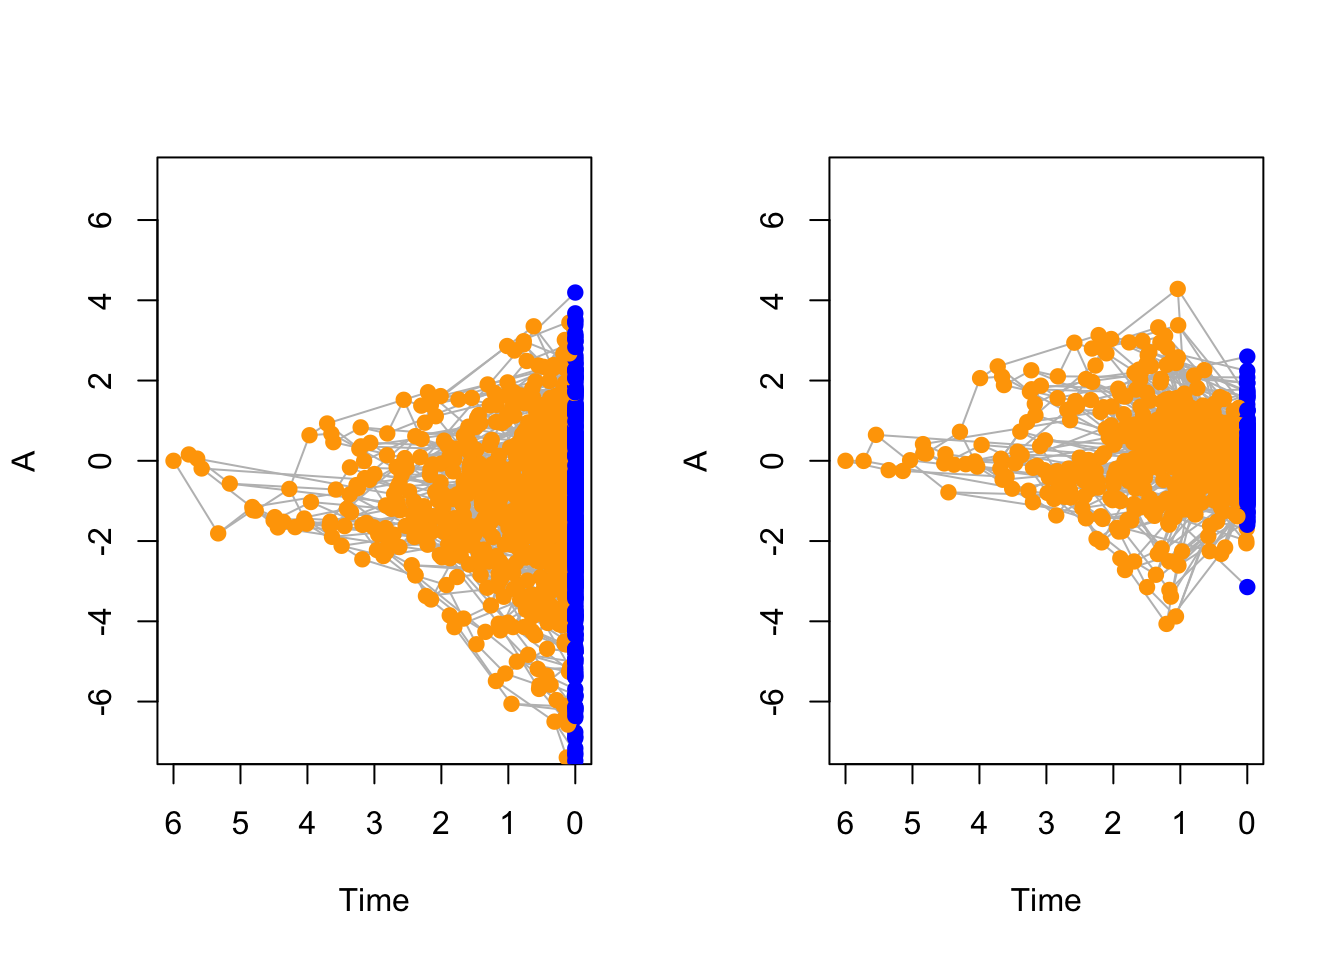
\includegraphics{dads_manual_files/figure-latex/unnamed-chunk-62-1.pdf}

\begin{Shaded}
\begin{Highlighting}[]
\CommentTok{# plot(no_event, trait = c(1:2))}
\CommentTok{# plot(change_correlation, trait = c(1:2), use.3D = TRUE)}
\end{Highlighting}
\end{Shaded}

\hypertarget{event-for-changing-a-modifier}{%
\subsection{Event for changing a modifier}\label{event-for-changing-a-modifier}}

\begin{Shaded}
\begin{Highlighting}[]
\CommentTok{## Set the parameters}
\NormalTok{stop.rule <-}\StringTok{ }\KeywordTok{list}\NormalTok{(}\DataTypeTok{max.time =} \DecValTok{4}\NormalTok{)}
\NormalTok{bd.params <-}\StringTok{ }\KeywordTok{list}\NormalTok{(}\DataTypeTok{extinction =} \DecValTok{0}\NormalTok{, }\DataTypeTok{speciation =} \DecValTok{1}\NormalTok{)}

\CommentTok{## Using a default trait and modifier object}
\NormalTok{modifiers <-}\StringTok{ }\KeywordTok{make.modifiers}\NormalTok{()}
\NormalTok{traits <-}\StringTok{ }\KeywordTok{make.traits}\NormalTok{()}

\CommentTok{## New condition and new modifier (increasing speciation if trait is negative)}
\NormalTok{new.condition <-}\StringTok{ }\ControlFlowTok{function}\NormalTok{(trait.values, lineage) \{}
    \KeywordTok{return}\NormalTok{(}\KeywordTok{parent.traits}\NormalTok{(trait.values, lineage) }\OperatorTok{<}\StringTok{ }\DecValTok{0}\NormalTok{)}
\NormalTok{\}}
\NormalTok{new.modify    <-}\StringTok{ }\ControlFlowTok{function}\NormalTok{(x, trait.values, lineage) \{}
  \KeywordTok{return}\NormalTok{(x }\OperatorTok{+}\StringTok{ }\DecValTok{1}\NormalTok{)}
\NormalTok{\}}

\CommentTok{## Update the modifier}
\NormalTok{change_speciation <-}\StringTok{ }\KeywordTok{make.events}\NormalTok{(}
    \DataTypeTok{condition    =} \KeywordTok{time.condition}\NormalTok{(}\DecValTok{3}\NormalTok{),}
    \DataTypeTok{target       =} \StringTok{"modifiers"}\NormalTok{,}
    \DataTypeTok{modification =} \KeywordTok{update.modifiers}\NormalTok{(}\DataTypeTok{speciation =}\NormalTok{ speciation,}
                                    \DataTypeTok{condition  =}\NormalTok{ new.condition,}
                                    \DataTypeTok{modify     =}\NormalTok{ new.modify))}

\KeywordTok{set.seed}\NormalTok{(}\DecValTok{4}\NormalTok{)}
\NormalTok{no_event <-}\StringTok{ }\KeywordTok{dads}\NormalTok{(}\DataTypeTok{bd.params =}\NormalTok{ bd.params,}
                 \DataTypeTok{stop.rule =}\NormalTok{ stop.rule,}
                 \DataTypeTok{traits    =}\NormalTok{ traits,}
                 \DataTypeTok{modifiers =}\NormalTok{ modifiers)}
\KeywordTok{set.seed}\NormalTok{(}\DecValTok{4}\NormalTok{)}
\NormalTok{change_spec <-}\StringTok{ }\KeywordTok{dads}\NormalTok{(}\DataTypeTok{bd.params =}\NormalTok{ bd.params,}
                    \DataTypeTok{stop.rule =}\NormalTok{ stop.rule,}
                    \DataTypeTok{traits    =}\NormalTok{ traits,}
                    \DataTypeTok{modifiers =}\NormalTok{ modifiers,}
                    \DataTypeTok{events    =}\NormalTok{ change_speciation)}

\CommentTok{## Visualise the results}
\KeywordTok{par}\NormalTok{(}\DataTypeTok{mfrow =} \KeywordTok{c}\NormalTok{(}\DecValTok{1}\NormalTok{,}\DecValTok{2}\NormalTok{))}
\KeywordTok{plot}\NormalTok{(no_event, }\DataTypeTok{main =} \StringTok{"No event"}\NormalTok{)}
\KeywordTok{plot}\NormalTok{(change_spec, }\DataTypeTok{main =} \StringTok{"Increase extinction for negative traits}\CharTok{\textbackslash{}n}\StringTok{after time 3"}\NormalTok{)}
\end{Highlighting}
\end{Shaded}

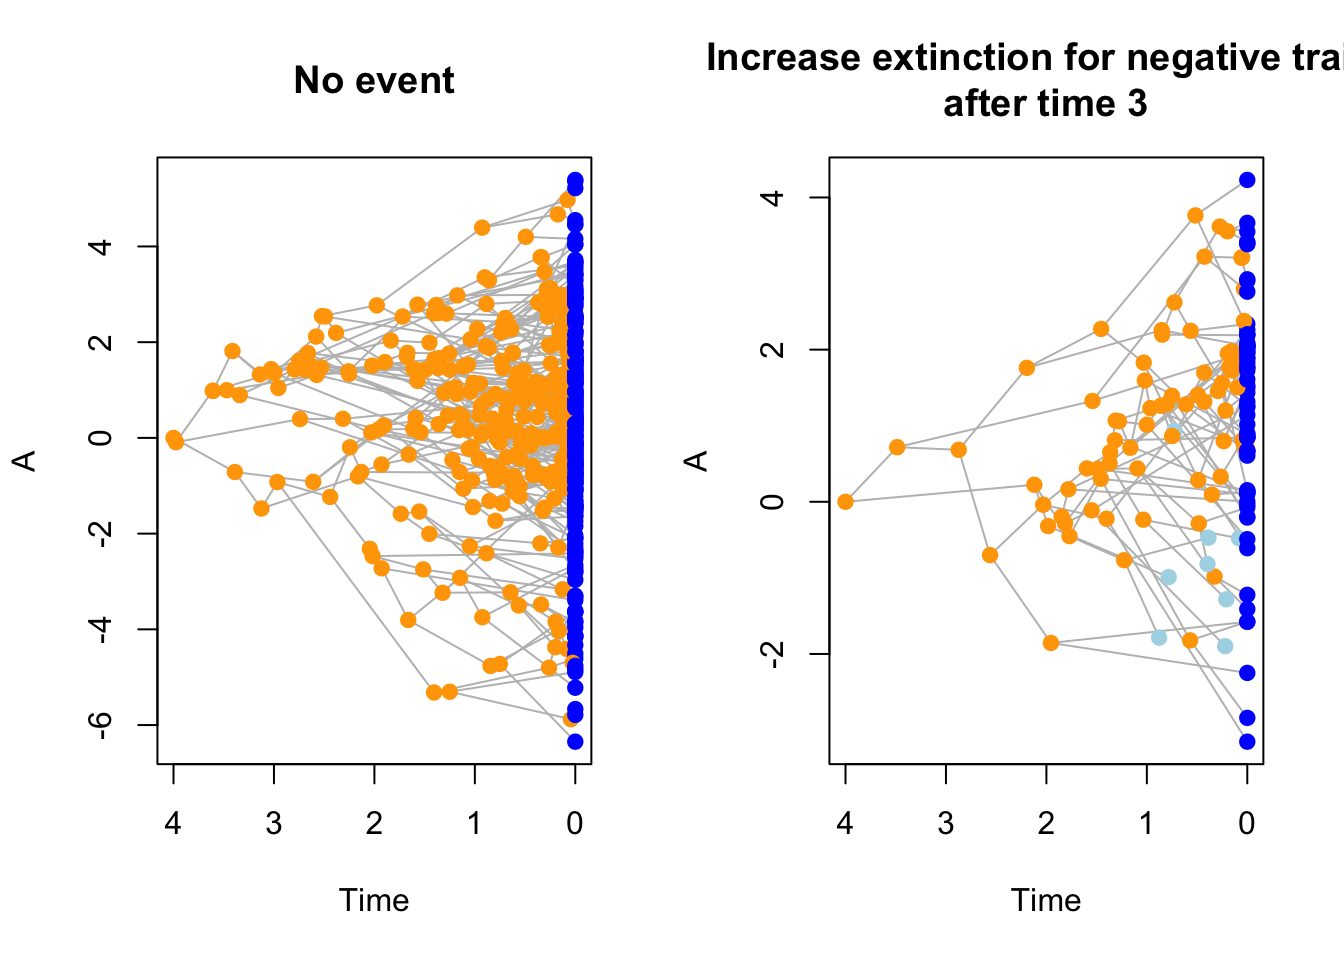
\includegraphics{dads_manual_files/figure-latex/unnamed-chunk-63-1.pdf}

\hypertarget{changing-branch-length-when-reaching-n-taxa}{%
\subsection{Changing branch length when reaching n taxa}\label{changing-branch-length-when-reaching-n-taxa}}

\begin{Shaded}
\begin{Highlighting}[]
\CommentTok{## Parameters}
\NormalTok{bd.params <-}\StringTok{ }\KeywordTok{list}\NormalTok{(}\DataTypeTok{extinction =} \DecValTok{0}\NormalTok{, }\DataTypeTok{speciation =} \DecValTok{1}\NormalTok{)}
\NormalTok{stop.rule <-}\StringTok{ }\KeywordTok{list}\NormalTok{(}\DataTypeTok{max.taxa =} \DecValTok{100}\NormalTok{)}
\NormalTok{modifiers <-}\StringTok{ }\KeywordTok{make.modifiers}\NormalTok{()}
\NormalTok{traits <-}\StringTok{ }\KeywordTok{make.traits}\NormalTok{()}

\CommentTok{## multiplying branch length 100 folds}
\NormalTok{new.modify <-}\StringTok{ }\ControlFlowTok{function}\NormalTok{(x, trait.values, lineage) \{}
  \KeywordTok{return}\NormalTok{(x }\OperatorTok{*}\StringTok{ }\DecValTok{100}\NormalTok{)}
\NormalTok{\}}

\CommentTok{## Event for increasing branch length after reaching 30 taxa}
\NormalTok{increase_brlen <-}\StringTok{ }\KeywordTok{make.events}\NormalTok{(}
                  \DataTypeTok{condition    =} \KeywordTok{taxa.condition}\NormalTok{(}\DecValTok{30}\NormalTok{),}
                  \DataTypeTok{target       =} \StringTok{"modifiers"}\NormalTok{,}
                  \DataTypeTok{modification =} \KeywordTok{update.modifiers}\NormalTok{(}
                                    \DataTypeTok{branch.length =}\NormalTok{ branch.length,}
                                    \DataTypeTok{modify =}\NormalTok{ new.modify))}

\CommentTok{## Run the simulations}
\KeywordTok{set.seed}\NormalTok{(}\DecValTok{5}\NormalTok{)}
\NormalTok{no_event <-}\StringTok{ }\KeywordTok{dads}\NormalTok{(}\DataTypeTok{bd.params =}\NormalTok{ bd.params,}
                 \DataTypeTok{stop.rule =}\NormalTok{ stop.rule,}
                 \DataTypeTok{traits    =}\NormalTok{ traits,}
                 \DataTypeTok{modifiers =}\NormalTok{ modifiers)}
\KeywordTok{set.seed}\NormalTok{(}\DecValTok{5}\NormalTok{)}
\NormalTok{increased_brlen <-}\StringTok{ }\KeywordTok{dads}\NormalTok{(}\DataTypeTok{bd.params =}\NormalTok{ bd.params,}
                        \DataTypeTok{stop.rule =}\NormalTok{ stop.rule,}
                        \DataTypeTok{traits    =}\NormalTok{ traits,}
                        \DataTypeTok{modifiers =}\NormalTok{ modifiers,}
                        \DataTypeTok{events    =}\NormalTok{ increase_brlen)}

\CommentTok{## Visualise the results}
\KeywordTok{par}\NormalTok{(}\DataTypeTok{mfrow =} \KeywordTok{c}\NormalTok{(}\DecValTok{1}\NormalTok{,}\DecValTok{2}\NormalTok{))}
\KeywordTok{plot}\NormalTok{(no_event, }\DataTypeTok{main =} \StringTok{"No event"}\NormalTok{)}
\KeywordTok{plot}\NormalTok{(increased_brlen, }\DataTypeTok{main =} \StringTok{"Increase branch length}\CharTok{\textbackslash{}n}\StringTok{after 30 taxa"}\NormalTok{)}
\end{Highlighting}
\end{Shaded}

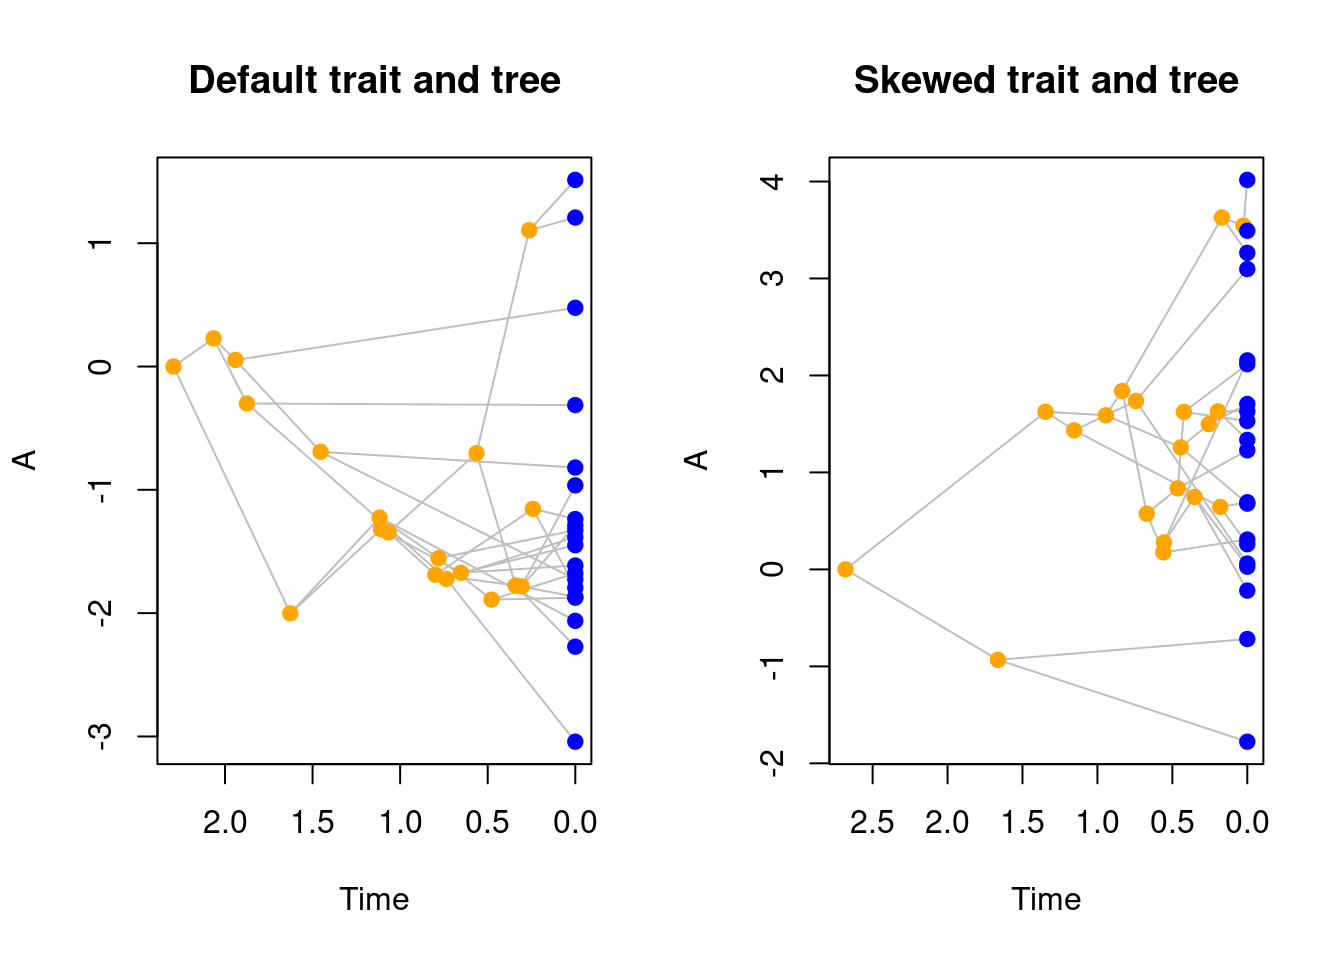
\includegraphics{dads_manual_files/figure-latex/unnamed-chunk-64-1.pdf}

\hypertarget{founding-event-a-subtree-with-no-fossils}{%
\subsection{Founding event: a subtree with no fossils}\label{founding-event-a-subtree-with-no-fossils}}

\begin{Shaded}
\begin{Highlighting}[]
\CommentTok{## Set up parameters}
\NormalTok{stop.rule <-}\StringTok{ }\KeywordTok{list}\NormalTok{(}\DataTypeTok{max.time =} \DecValTok{4}\NormalTok{)}
\NormalTok{bd.params <-}\StringTok{ }\KeywordTok{list}\NormalTok{(}\DataTypeTok{speciation =} \DecValTok{1}\NormalTok{, }\DataTypeTok{extinction =} \FloatTok{0.3}\NormalTok{)}

\CommentTok{## Events that generate a new process (founding effects)}
\NormalTok{founding_event <-}\StringTok{ }\KeywordTok{make.events}\NormalTok{(}
                  \DataTypeTok{condition    =} \KeywordTok{taxa.condition}\NormalTok{(}\DecValTok{10}\NormalTok{),}
                  \DataTypeTok{target       =} \StringTok{"founding"}\NormalTok{,}
                  \DataTypeTok{modification =} \KeywordTok{founding.event}\NormalTok{(}
                                    \DataTypeTok{bd.params =} \KeywordTok{list}\NormalTok{(}\DataTypeTok{speciation =} \DecValTok{2}\NormalTok{,}
                                                     \DataTypeTok{extinction =} \DecValTok{0}\NormalTok{)),}
                  \DataTypeTok{additional.args =} \KeywordTok{list}\NormalTok{(}\DataTypeTok{prefix =} \StringTok{"founding_"}\NormalTok{))}
    
\CommentTok{## Simulations}
\KeywordTok{set.seed}\NormalTok{(}\DecValTok{11}\NormalTok{)}
\NormalTok{founding_tree <-}\StringTok{ }\KeywordTok{dads}\NormalTok{(}\DataTypeTok{bd.params =}\NormalTok{ bd.params,}
                      \DataTypeTok{stop.rule =}\NormalTok{ stop.rule,}
                      \DataTypeTok{events    =}\NormalTok{ founding_event)}
\KeywordTok{plot}\NormalTok{(founding_tree, }\DataTypeTok{cex =} \FloatTok{0.4}\NormalTok{)}
\end{Highlighting}
\end{Shaded}

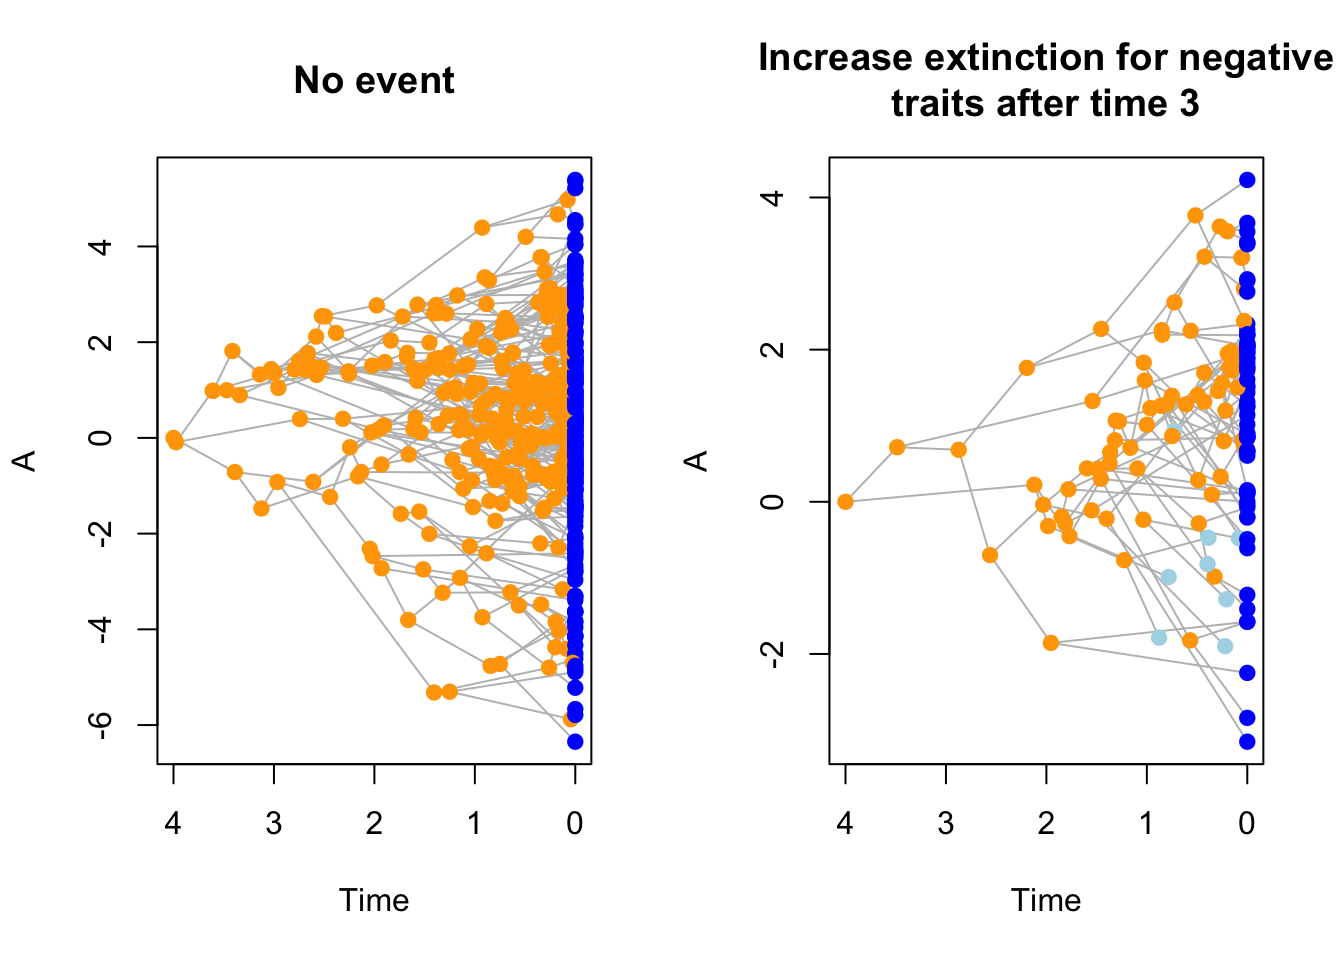
\includegraphics{dads_manual_files/figure-latex/unnamed-chunk-65-1.pdf}

\hypertarget{founding-event-with-traits}{%
\subsection{Founding event with traits}\label{founding-event-with-traits}}

\begin{Shaded}
\begin{Highlighting}[]
\CommentTok{## Set up parameters}
\NormalTok{stop.rule <-}\StringTok{ }\KeywordTok{list}\NormalTok{(}\DataTypeTok{max.time =} \DecValTok{4}\NormalTok{)}
\NormalTok{bd.params <-}\StringTok{ }\KeywordTok{list}\NormalTok{(}\DataTypeTok{speciation =} \DecValTok{1}\NormalTok{, }\DataTypeTok{extinction =} \FloatTok{0.3}\NormalTok{)}
\NormalTok{traits    <-}\StringTok{ }\KeywordTok{make.traits}\NormalTok{()}

\CommentTok{## Events that generate a new process (founding effects)}
\NormalTok{founding_event <-}\StringTok{ }\KeywordTok{make.events}\NormalTok{(}
                  \DataTypeTok{condition    =} \KeywordTok{taxa.condition}\NormalTok{(}\DecValTok{10}\NormalTok{),}
                  \DataTypeTok{target       =} \StringTok{"founding"}\NormalTok{,}
                  \DataTypeTok{modification =} \KeywordTok{founding.event}\NormalTok{(}
                                    \DataTypeTok{bd.params =} \KeywordTok{list}\NormalTok{(}\DataTypeTok{speciation =} \DecValTok{2}\NormalTok{,}
                                                     \DataTypeTok{extinction =} \DecValTok{0}\NormalTok{),}
                                    \DataTypeTok{traits =} \KeywordTok{make.traits}\NormalTok{(}\DataTypeTok{process =}\NormalTok{ OU.process)),}
                  \DataTypeTok{additional.args =} \KeywordTok{list}\NormalTok{(}\DataTypeTok{prefix =} \StringTok{"founding_"}\NormalTok{))}

\CommentTok{## Simulating the tree}
\KeywordTok{set.seed}\NormalTok{(}\DecValTok{19}\NormalTok{)}
\NormalTok{founding_tree <-}\StringTok{ }\KeywordTok{dads}\NormalTok{(}\DataTypeTok{bd.params =}\NormalTok{ bd.params,}
                      \DataTypeTok{stop.rule =}\NormalTok{ stop.rule,}
                      \DataTypeTok{traits    =} \KeywordTok{make.traits}\NormalTok{(),}
                      \DataTypeTok{events    =}\NormalTok{ founding_event)}
\KeywordTok{plot}\NormalTok{(founding_tree)}
\end{Highlighting}
\end{Shaded}

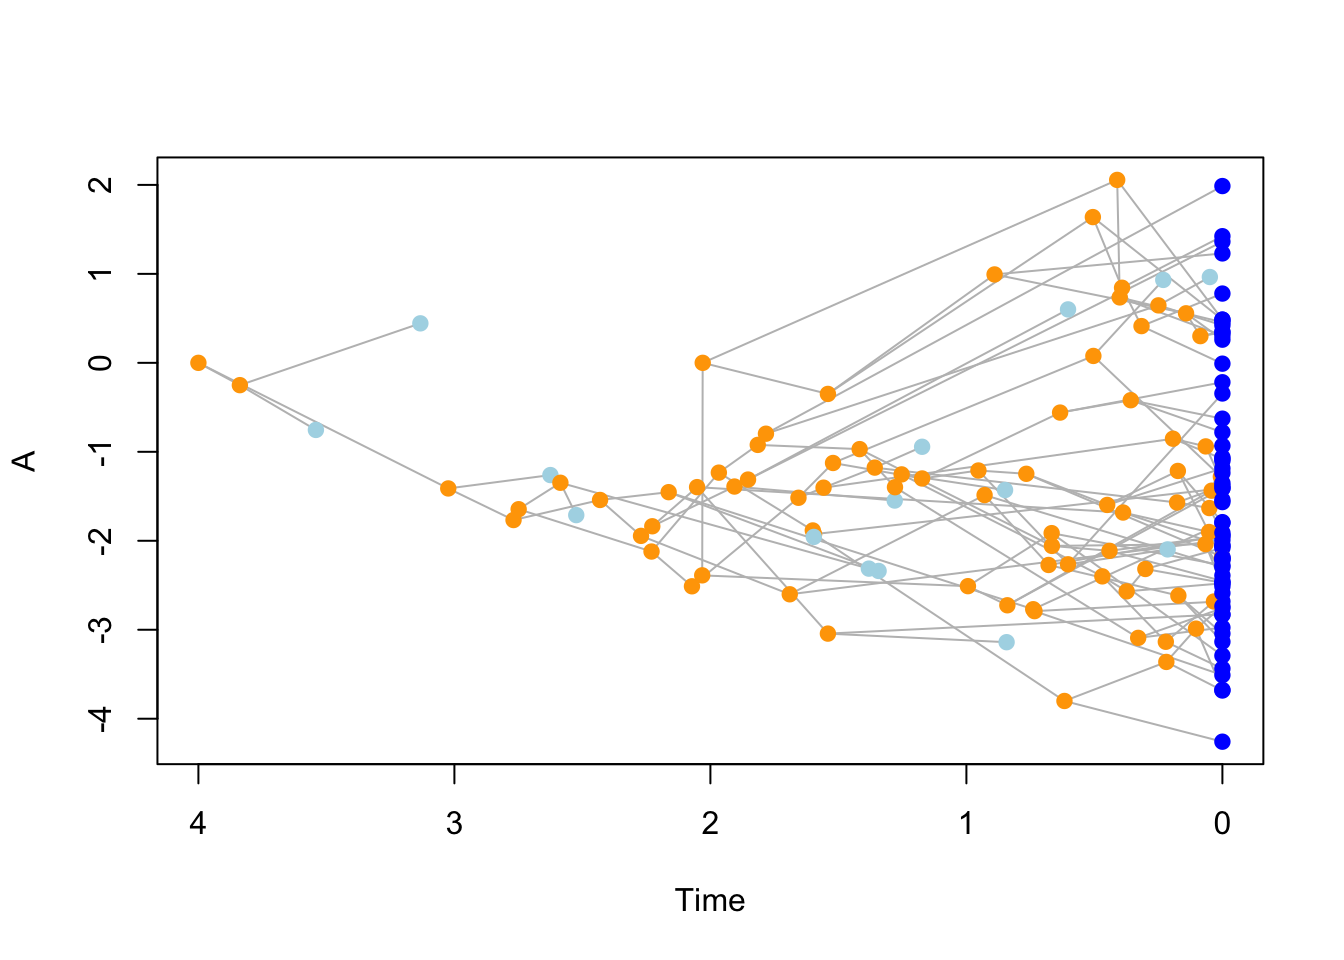
\includegraphics{dads_manual_files/figure-latex/unnamed-chunk-66-1.pdf}

\hypertarget{thorough-example}{%
\chapter{Thorough example}\label{thorough-example}}

Here we are going to look at an example on how to simulate complex evolutionary histories with \texttt{dads}.

Let say we want to simulate the following story:

\begin{enumerate}
\def\labelenumi{\arabic{enumi}.}
\tightlist
\item
  A lineage evolves in a normal birth-death fashion (with extinction) from a single origin and with two traits called:

  \begin{itemize}
  \tightlist
  \item
    ``Distance'': the physical distance between species in an arbitrary 1D space (evolving in a Brownian motion).
  \item
    ``Variable'': a 2D uncorrelated Ornstein-Uhlenbeck trait that corresponds to some traits the lineages have.
    During the whole process, lineages that are more further away from the other species in terms of distance have a higher change of speciating (proportional to that distance).
  \end{itemize}
\end{enumerate}

Three events then happen during the evolutionary history of this lineage:

\begin{enumerate}
\def\labelenumi{\arabic{enumi}.}
\setcounter{enumi}{1}
\tightlist
\item
  ``Correlation event'': after reaching a certain number of taxa an event happens making the ``Variables'' trait dimensions become correlated.
\item
  ``Selective extinction event'': after reaching a certain point in time, lineages with their ``Variables'' values that are negative go extinct
\item
  ``Founding event'': after reaching a value for the ``Distance'' trait, a founding event happens with a new birth-death process with no extinction and where the ``Variable'' is now a 2D correlated Brownian Motion.
\item
  ``Mass extinction event'': after reaching a certain number of taxa in the ``Founding event'', 80\% of taxa go extinct randomly.
\end{enumerate}

We are going to run each step one by one in a cumulative manner to see how they pile up:

\hypertarget{step-1}{%
\section{Step 1:}\label{step-1}}

\hypertarget{the-birth-death-parameters}{%
\subsection{The birth death parameters}\label{the-birth-death-parameters}}

First let's set the overall birth death parameters (a speciation of 1.2 and an extinction of 0.3):

\begin{Shaded}
\begin{Highlighting}[]
\CommentTok{## The birth death parameters}
\NormalTok{bd_params <-}\StringTok{ }\KeywordTok{list}\NormalTok{(}\DataTypeTok{speciation =} \FloatTok{1.2}\NormalTok{, }\DataTypeTok{extinction =} \FloatTok{0.3}\NormalTok{)}
\CommentTok{## The stopping rule}
\NormalTok{stop_rule <-}\StringTok{ }\KeywordTok{list}\NormalTok{(}\DataTypeTok{max.time =} \DecValTok{4}\NormalTok{)}
\end{Highlighting}
\end{Shaded}

And let's quickly test if the simulation works by running a birth death tree without traits and anything:

\begin{Shaded}
\begin{Highlighting}[]
\KeywordTok{set.seed}\NormalTok{(}\DecValTok{0}\NormalTok{) }\CommentTok{# 123 also works}
\CommentTok{## Running a birth death tree }
\NormalTok{results <-}\StringTok{ }\KeywordTok{dads}\NormalTok{(}\DataTypeTok{bd.params =}\NormalTok{ bd_params,}
                \DataTypeTok{stop.rule =}\NormalTok{ stop_rule)}

\CommentTok{## And displaying the results}
\KeywordTok{plot}\NormalTok{(results)}
\KeywordTok{axisPhylo}\NormalTok{()}
\end{Highlighting}
\end{Shaded}

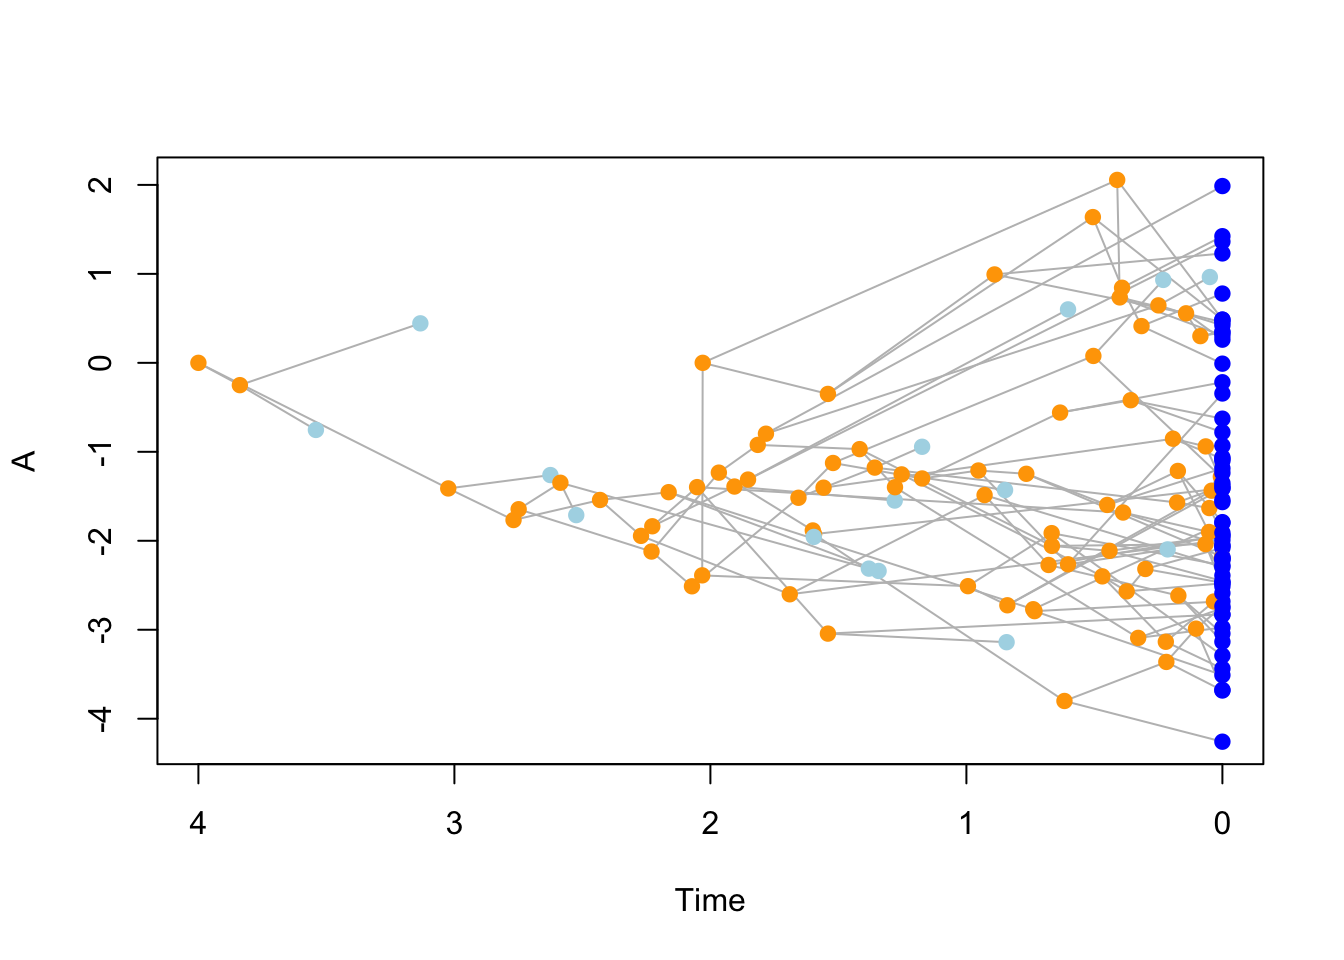
\includegraphics{dads_manual_files/figure-latex/unnamed-chunk-68-1.pdf}

\hypertarget{the-traits}{%
\subsection{The traits}\label{the-traits}}

Then let's create the traits:

\begin{Shaded}
\begin{Highlighting}[]
\CommentTok{## The trait object}
\NormalTok{two_traits <-}\StringTok{ }\KeywordTok{make.traits}\NormalTok{(}\DataTypeTok{process =} \KeywordTok{c}\NormalTok{(BM.process, OU.process), }\DataTypeTok{n =} \KeywordTok{c}\NormalTok{(}\DecValTok{1}\NormalTok{, }\DecValTok{2}\NormalTok{),}
                          \DataTypeTok{trait.names =} \KeywordTok{c}\NormalTok{(}\StringTok{"Distance"}\NormalTok{, }\StringTok{"Variables"}\NormalTok{))}
\end{Highlighting}
\end{Shaded}

\begin{Shaded}
\begin{Highlighting}[]
\CommentTok{## Visualise the 1D trait (BM.process)}
\KeywordTok{plot}\NormalTok{(two_traits, }\DataTypeTok{trait =} \DecValTok{1}\NormalTok{)}
\end{Highlighting}
\end{Shaded}

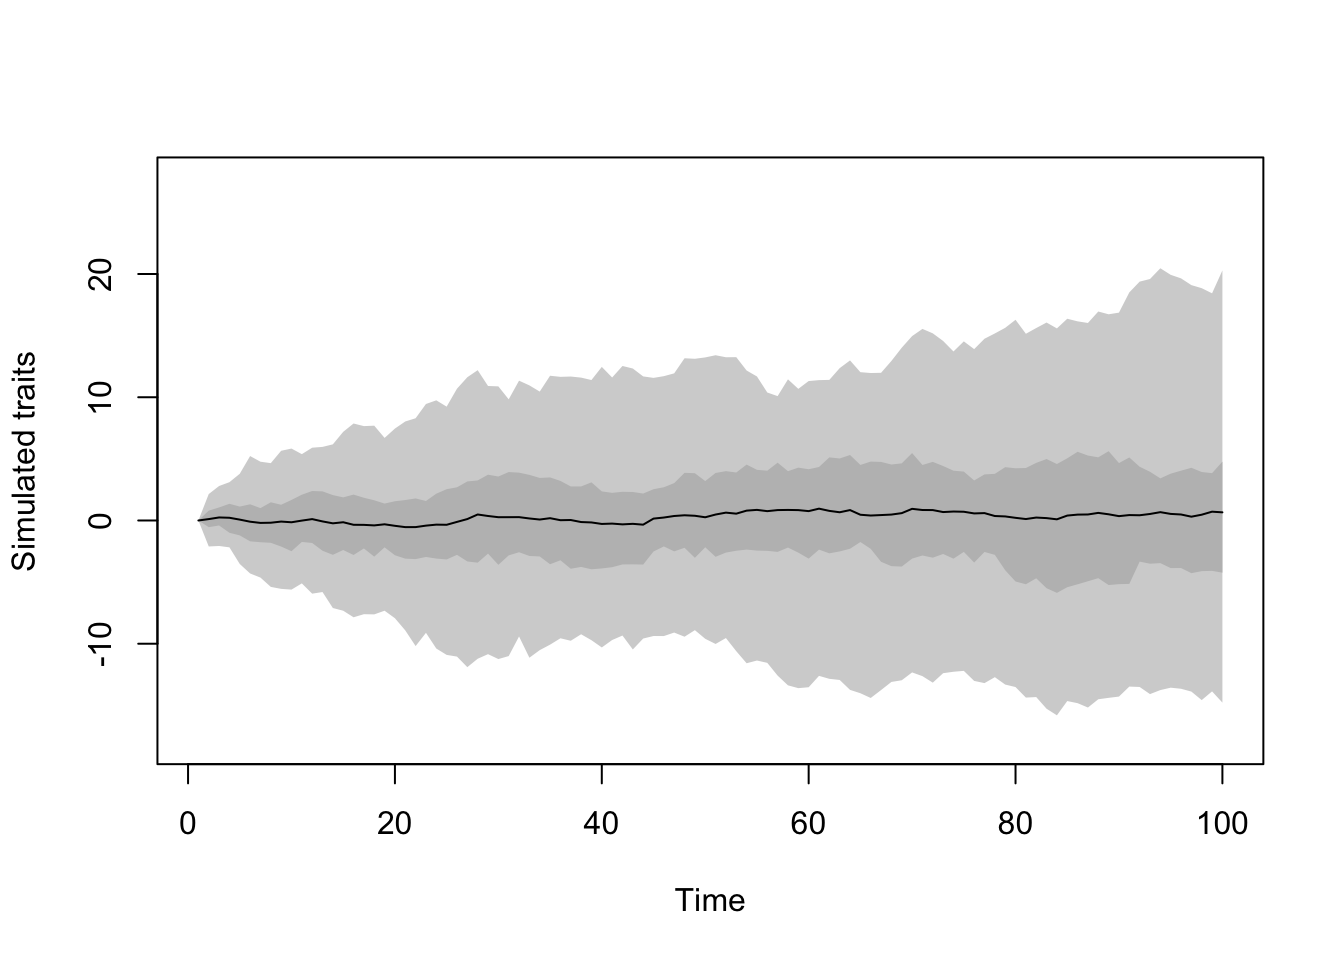
\includegraphics{dads_manual_files/figure-latex/unnamed-chunk-70-1.pdf}

\begin{Shaded}
\begin{Highlighting}[]
\CommentTok{## Visualise the 2D trait (uncorrelated OU.process)}
\KeywordTok{plot}\NormalTok{(two_traits, }\DataTypeTok{trait =} \DecValTok{2}\NormalTok{, }\DataTypeTok{use.3D =} \OtherTok{TRUE}\NormalTok{)}
\end{Highlighting}
\end{Shaded}

Note that specifying the correlation matrix is not necessary here \emph{per se} (since no correlation is the default) but we will modify it through an event later on so it's good practice to have it properly stated before hand (to avoid any confusion).

We can then run the tree with the traits:

\begin{Shaded}
\begin{Highlighting}[]
\KeywordTok{set.seed}\NormalTok{(}\DecValTok{0}\NormalTok{)}
\CommentTok{## Running a birth death tree }
\NormalTok{results <-}\StringTok{ }\KeywordTok{dads}\NormalTok{(}\DataTypeTok{bd.params  =}\NormalTok{ bd_params,}
                \DataTypeTok{stop.rule  =}\NormalTok{ stop_rule,}
                \DataTypeTok{traits     =}\NormalTok{ two_traits)}

\CommentTok{## And displaying the results}
\KeywordTok{par}\NormalTok{(}\DataTypeTok{mfrow =} \KeywordTok{c}\NormalTok{(}\DecValTok{1}\NormalTok{,}\DecValTok{2}\NormalTok{))}
\KeywordTok{plot}\NormalTok{(results, }\DataTypeTok{trait =} \DecValTok{1}\NormalTok{, }\DataTypeTok{main =} \StringTok{"Trait 1: Distance"}\NormalTok{)}
\KeywordTok{plot}\NormalTok{(results, }\DataTypeTok{trait =} \KeywordTok{c}\NormalTok{(}\DecValTok{2}\NormalTok{,}\DecValTok{3}\NormalTok{), }\DataTypeTok{main =} \StringTok{"Variables correlation"}\NormalTok{)}
\end{Highlighting}
\end{Shaded}

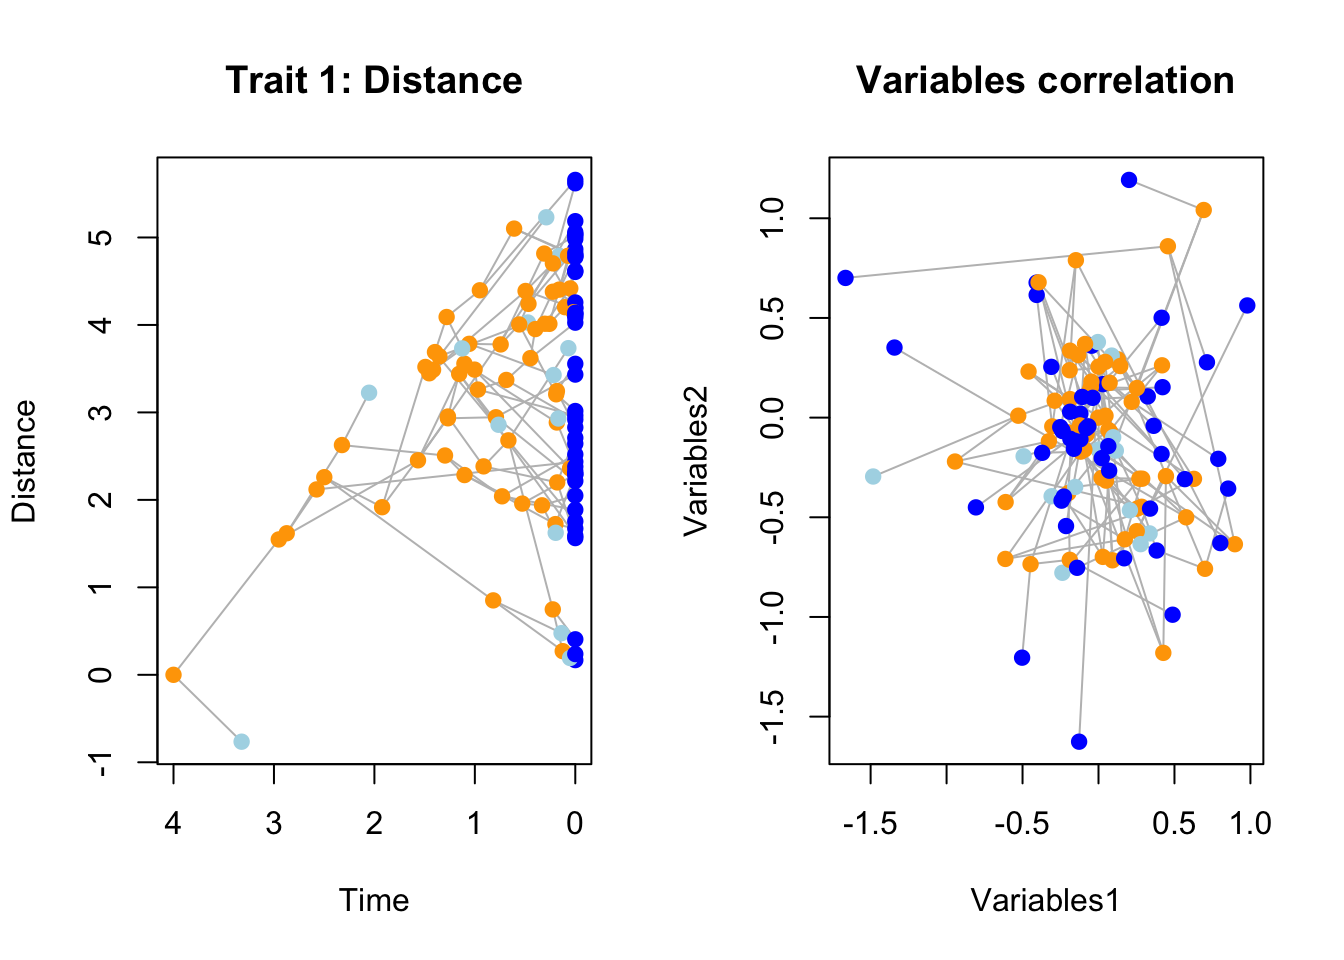
\includegraphics{dads_manual_files/figure-latex/unnamed-chunk-72-1.pdf}

\begin{Shaded}
\begin{Highlighting}[]
\CommentTok{## Visualising the tree in 3D}
\KeywordTok{plot}\NormalTok{(results, }\DataTypeTok{trait =} \KeywordTok{c}\NormalTok{(}\DecValTok{2}\NormalTok{,}\DecValTok{3}\NormalTok{), }\DataTypeTok{use.3D =} \OtherTok{TRUE}\NormalTok{)}
\end{Highlighting}
\end{Shaded}

\hypertarget{the-modifiers}{%
\subsection{The modifiers}\label{the-modifiers}}

\begin{Shaded}
\begin{Highlighting}[]
\CommentTok{## Speciation event is more likely if lineage's ancestor is further away from the mean trait value}
\NormalTok{distance.modify <-}\StringTok{ }\ControlFlowTok{function}\NormalTok{(x, trait.values, lineage) }\KeywordTok{return}\NormalTok{(x }\OperatorTok{+}\StringTok{ }\NormalTok{x }\OperatorTok{*}\StringTok{ }\KeywordTok{abs}\NormalTok{(}\KeywordTok{parent.traits}\NormalTok{(trait.values, lineage)[}\DecValTok{1}\NormalTok{] }\OperatorTok{-}\StringTok{ }\KeywordTok{mean}\NormalTok{(trait.values[,}\DecValTok{1}\NormalTok{])))}

\CommentTok{## Make a distance modifier}
\NormalTok{distance.speciation <-}\StringTok{ }\KeywordTok{make.modifiers}\NormalTok{(}\DataTypeTok{speciation =}\NormalTok{ speciation,}
                                      \DataTypeTok{modify =}\NormalTok{ distance.modify)}
\end{Highlighting}
\end{Shaded}

\begin{Shaded}
\begin{Highlighting}[]
\KeywordTok{set.seed}\NormalTok{(}\DecValTok{42}\NormalTok{)}
\CommentTok{## Running a birth death tree }
\NormalTok{results <-}\StringTok{ }\KeywordTok{dads}\NormalTok{(}\DataTypeTok{bd.params  =}\NormalTok{ bd_params,}
                \DataTypeTok{stop.rule  =}\NormalTok{ stop_rule,}
                \DataTypeTok{traits     =}\NormalTok{ two_traits,}
                \DataTypeTok{modifiers  =}\NormalTok{ distance.speciation)}

\CommentTok{## And displaying the results}
\KeywordTok{par}\NormalTok{(}\DataTypeTok{mfrow =} \KeywordTok{c}\NormalTok{(}\DecValTok{1}\NormalTok{,}\DecValTok{2}\NormalTok{))}
\KeywordTok{plot}\NormalTok{(results, }\DataTypeTok{trait =} \DecValTok{1}\NormalTok{, }\DataTypeTok{main =} \StringTok{"Trait 1: Distance"}\NormalTok{)}
\KeywordTok{plot}\NormalTok{(results, }\DataTypeTok{trait =} \KeywordTok{c}\NormalTok{(}\DecValTok{2}\NormalTok{,}\DecValTok{3}\NormalTok{), }\DataTypeTok{main =} \StringTok{"Variables correlation"}\NormalTok{)}
\end{Highlighting}
\end{Shaded}

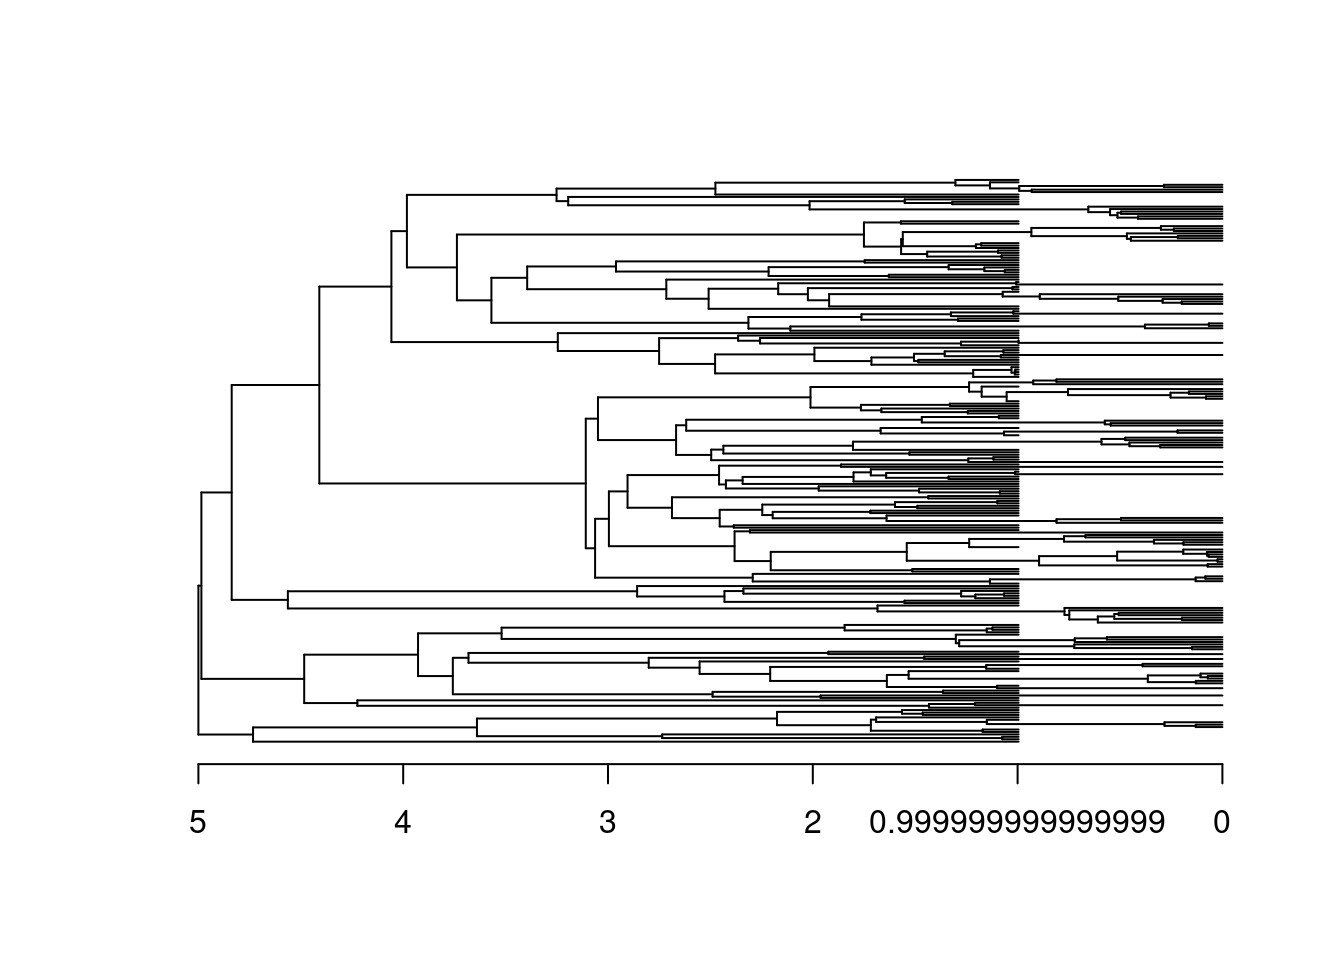
\includegraphics{dads_manual_files/figure-latex/unnamed-chunk-75-1.pdf}

\hypertarget{step-2}{%
\section{Step 2:}\label{step-2}}

\begin{enumerate}
\def\labelenumi{\arabic{enumi}.}
\setcounter{enumi}{1}
\tightlist
\item
  ``Correlation event'': after reaching a certain number of taxa an event happens making the ``Variable'' trait dimensions become correlated.
\end{enumerate}

\begin{Shaded}
\begin{Highlighting}[]
\CommentTok{## The correlation change event}
\NormalTok{events_list <-}\StringTok{ }\KeywordTok{make.events}\NormalTok{(}\DataTypeTok{event.name   =} \StringTok{"Correlation"}\NormalTok{,}
                           \DataTypeTok{target       =} \StringTok{"traits"}\NormalTok{,}
                           \DataTypeTok{condition    =} \KeywordTok{taxa.condition}\NormalTok{(}\DecValTok{30}\NormalTok{),}
                           \DataTypeTok{modification =} \KeywordTok{update.traits}\NormalTok{(}
                    \DataTypeTok{process.args =} \KeywordTok{list}\NormalTok{(}\DataTypeTok{Sigma =} \KeywordTok{matrix}\NormalTok{(}\KeywordTok{c}\NormalTok{(}\FloatTok{0.7}\NormalTok{, }\DecValTok{0}\NormalTok{, }\DecValTok{0}\NormalTok{, }\FloatTok{0.7}\NormalTok{), }\DecValTok{2}\NormalTok{, }\DecValTok{2}\NormalTok{)),}
                    \DataTypeTok{trait.names  =} \StringTok{"Variables"}\NormalTok{))}
\end{Highlighting}
\end{Shaded}

\begin{Shaded}
\begin{Highlighting}[]
\KeywordTok{set.seed}\NormalTok{(}\DecValTok{8}\NormalTok{)}
\CommentTok{## Running a birth death tree }
\NormalTok{results <-}\StringTok{ }\KeywordTok{dads}\NormalTok{(}\DataTypeTok{bd.params  =}\NormalTok{ bd_params,}
                \DataTypeTok{stop.rule  =}\NormalTok{ stop_rule,}
                \DataTypeTok{traits     =}\NormalTok{ two_traits,}
                \DataTypeTok{modifiers  =}\NormalTok{ distance.speciation,}
                \DataTypeTok{events     =}\NormalTok{ events_list)}

\CommentTok{## And displaying the results}
\KeywordTok{par}\NormalTok{(}\DataTypeTok{mfrow =} \KeywordTok{c}\NormalTok{(}\DecValTok{1}\NormalTok{,}\DecValTok{2}\NormalTok{))}
\KeywordTok{plot}\NormalTok{(results, }\DataTypeTok{trait =} \DecValTok{1}\NormalTok{, }\DataTypeTok{main =} \StringTok{"Trait 1: Distance"}\NormalTok{)}
\KeywordTok{plot}\NormalTok{(results, }\DataTypeTok{trait =} \KeywordTok{c}\NormalTok{(}\DecValTok{2}\NormalTok{,}\DecValTok{3}\NormalTok{), }\DataTypeTok{main =} \StringTok{"Variables correlation"}\NormalTok{)}
\end{Highlighting}
\end{Shaded}

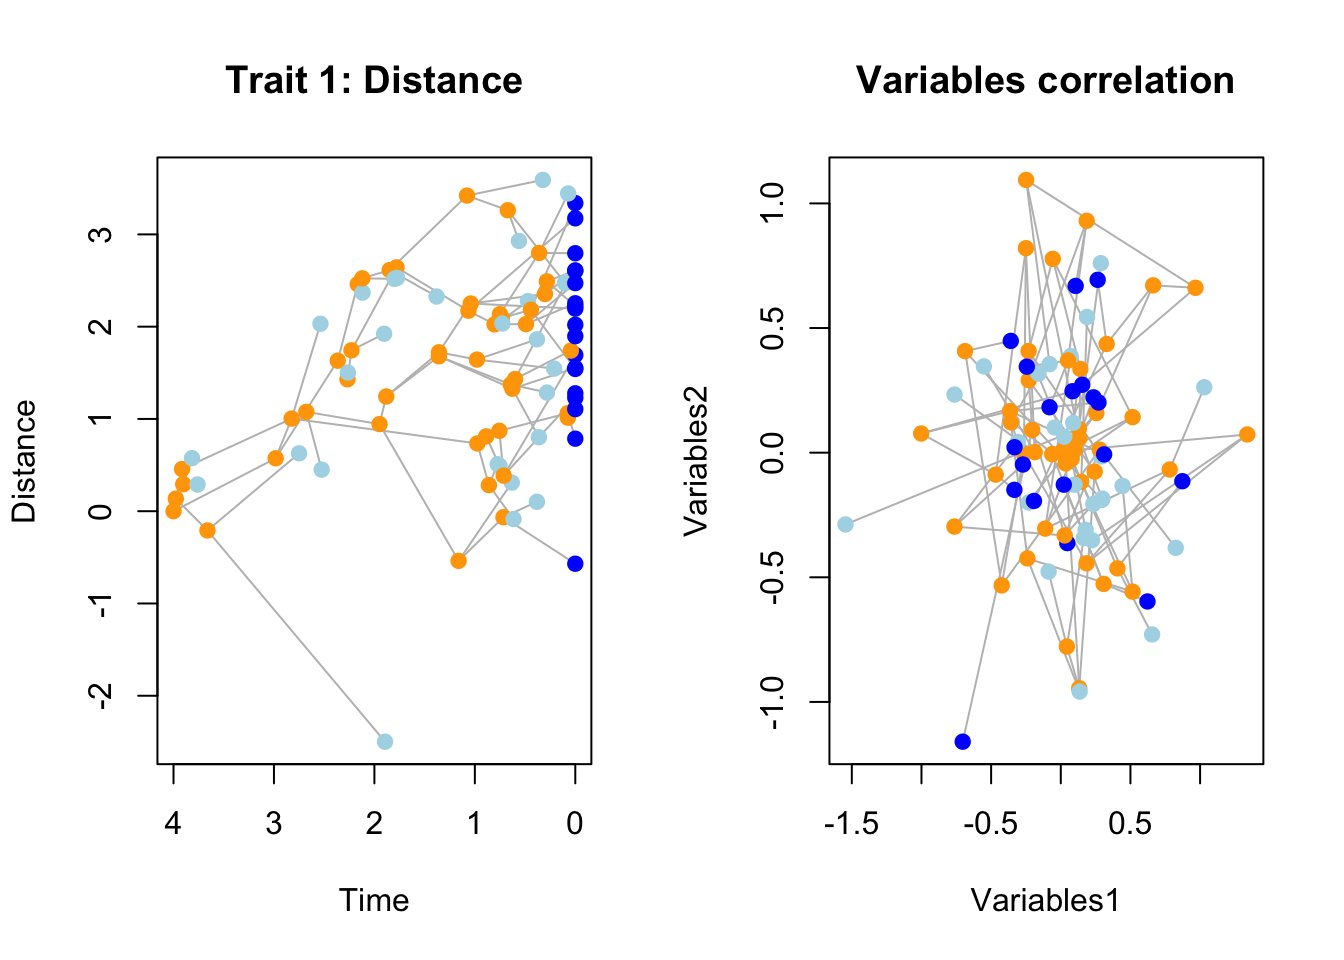
\includegraphics{dads_manual_files/figure-latex/unnamed-chunk-77-1.pdf}

\begin{Shaded}
\begin{Highlighting}[]
\CommentTok{## Visualising the tree in 3D}
\KeywordTok{plot}\NormalTok{(results, }\DataTypeTok{trait =} \KeywordTok{c}\NormalTok{(}\DecValTok{2}\NormalTok{,}\DecValTok{3}\NormalTok{), }\DataTypeTok{use.3D =} \OtherTok{TRUE}\NormalTok{)}
\end{Highlighting}
\end{Shaded}

\hypertarget{step-3}{%
\section{Step 3:}\label{step-3}}

\begin{enumerate}
\def\labelenumi{\arabic{enumi}.}
\setcounter{enumi}{2}
\tightlist
\item
  ``Selective extinction event'': after reaching a certain point in time, lineages with their ``Variables'' values that are negative go extinct
\end{enumerate}

\hypertarget{bugged-from-here}{%
\chapter{BUGGED FROM HERE}\label{bugged-from-here}}

\begin{Shaded}
\begin{Highlighting}[]
\CommentTok{## Adding the selective event}
\NormalTok{events_list <-}\StringTok{ }\KeywordTok{make.events}\NormalTok{(}\DataTypeTok{event.name   =} \StringTok{"Selection"}\NormalTok{,}
                           \DataTypeTok{add          =}\NormalTok{ events_list,}
                           \DataTypeTok{target       =} \StringTok{"taxa"}\NormalTok{,}
                           \DataTypeTok{condition    =} \KeywordTok{time.condition}\NormalTok{(}\DecValTok{4}\NormalTok{),}
                           \DataTypeTok{modification =} \KeywordTok{trait.extinction}\NormalTok{(}\DataTypeTok{x =} \DecValTok{0}\NormalTok{, }\DataTypeTok{condition =} \StringTok{`}\DataTypeTok{<}\StringTok{`}\NormalTok{, }\DataTypeTok{trait =} \DecValTok{2}\NormalTok{))}
\end{Highlighting}
\end{Shaded}

Problem with \texttt{modification} argument here

\begin{Shaded}
\begin{Highlighting}[]
\CommentTok{## Running a birth death tree }
\NormalTok{results <-}\StringTok{ }\KeywordTok{dads}\NormalTok{(}\DataTypeTok{bd.params  =}\NormalTok{ bd_params,}
                \DataTypeTok{stop.rule  =}\NormalTok{ stop_rule,}
                \DataTypeTok{traits     =}\NormalTok{ two_traits,}
                \DataTypeTok{modifiers  =}\NormalTok{ distance.speciation,}
                \DataTypeTok{events     =}\NormalTok{ events_list)}

\CommentTok{## And displaying the results}
\KeywordTok{par}\NormalTok{(}\DataTypeTok{mfrow =} \KeywordTok{c}\NormalTok{(}\DecValTok{1}\NormalTok{,}\DecValTok{2}\NormalTok{))}
\KeywordTok{plot}\NormalTok{(results, }\DataTypeTok{trait =} \DecValTok{1}\NormalTok{, }\DataTypeTok{main =} \StringTok{"Trait 1: Distance"}\NormalTok{)}
\KeywordTok{plot}\NormalTok{(results, }\DataTypeTok{trait =} \KeywordTok{c}\NormalTok{(}\DecValTok{2}\NormalTok{,}\DecValTok{3}\NormalTok{), }\DataTypeTok{main =} \StringTok{"Variables correlation"}\NormalTok{)}
\end{Highlighting}
\end{Shaded}

\hypertarget{step-4-and-5}{%
\section{Step 4 and 5:}\label{step-4-and-5}}

\begin{enumerate}
\def\labelenumi{\arabic{enumi}.}
\setcounter{enumi}{3}
\tightlist
\item
  ``Founding event'': after reaching a value for the ``Distance'' trait, a founding event happens with a new birth-death process with no extinction and where the ``Variable'' is now a 2D correlated Brownian Motion.
\item
  ``Mass extinction event'': after reaching a certain number of taxa in the ``Founding event'', 80\% of taxa go extinct randomly.
\end{enumerate}

\begin{Shaded}
\begin{Highlighting}[]
\CommentTok{## The new trait for the founding event}
\NormalTok{new_traits <-}\StringTok{ }\KeywordTok{make.traits}\NormalTok{(}\DataTypeTok{process =} \KeywordTok{c}\NormalTok{(BM.process, BM.process), }\DataTypeTok{n =} \KeywordTok{c}\NormalTok{(}\DecValTok{1}\NormalTok{, }\DecValTok{2}\NormalTok{),}
                          \DataTypeTok{trait.names =} \KeywordTok{c}\NormalTok{(}\StringTok{"Distance"}\NormalTok{, }\StringTok{"Variables"}\NormalTok{))}

\CommentTok{## The mass extinction event after reaching 50 taxa}
\NormalTok{mass_extinction <-}\StringTok{ }\KeywordTok{make.events}\NormalTok{(}\DataTypeTok{target       =} \StringTok{"taxa"}\NormalTok{,}
                               \DataTypeTok{condition    =} \KeywordTok{taxa.condition}\NormalTok{(}\DecValTok{50}\NormalTok{),}
                               \DataTypeTok{modification =} \KeywordTok{random.extinction}\NormalTok{(}\FloatTok{0.8}\NormalTok{))}
\end{Highlighting}
\end{Shaded}

\begin{Shaded}
\begin{Highlighting}[]
\CommentTok{## The selective event}
\NormalTok{events_list <-}\StringTok{ }\KeywordTok{make.events}\NormalTok{(}\DataTypeTok{event.name   =} \StringTok{"Founding"}\NormalTok{, }
                           \DataTypeTok{add          =}\NormalTok{ events_list,}
                           \DataTypeTok{target       =} \StringTok{"founding"}\NormalTok{,}
                           \DataTypeTok{condition    =} \KeywordTok{trait.condition}\NormalTok{(}\DecValTok{3}\NormalTok{),}
                           \DataTypeTok{modification =} \KeywordTok{founding.event}\NormalTok{(}\DataTypeTok{traits    =}\NormalTok{ new_traits,}
                                                         \DataTypeTok{events    =}\NormalTok{ mass_extinction,}
                                                         \DataTypeTok{bd.params =} \KeywordTok{list}\NormalTok{(}
                                                            \DataTypeTok{speciation =} \DecValTok{2}\NormalTok{,}
                                                            \DataTypeTok{extinction =} \DecValTok{0}\NormalTok{)),}
                           \DataTypeTok{additional.args =} \KeywordTok{list}\NormalTok{(}\DataTypeTok{prefix =} \StringTok{"found_"}\NormalTok{))}
\end{Highlighting}
\end{Shaded}

\begin{Shaded}
\begin{Highlighting}[]
\CommentTok{## Running a birth death tree }
\NormalTok{results <-}\StringTok{ }\KeywordTok{dads}\NormalTok{(}\DataTypeTok{bd.params  =}\NormalTok{ bd_params,}
                \DataTypeTok{stop.rule  =}\NormalTok{ stop_rule,}
                \DataTypeTok{traits     =}\NormalTok{ two_traits,}
                \DataTypeTok{modifiers  =}\NormalTok{ distance.speciation,}
                \DataTypeTok{events     =}\NormalTok{ events_list,}
                \DataTypeTok{null.error =} \DecValTok{100}\NormalTok{)}

\CommentTok{## And displaying the results}
\KeywordTok{par}\NormalTok{(}\DataTypeTok{mfrow =} \KeywordTok{c}\NormalTok{(}\DecValTok{1}\NormalTok{,}\DecValTok{2}\NormalTok{))}
\KeywordTok{plot}\NormalTok{(results, }\DataTypeTok{trait =} \DecValTok{1}\NormalTok{, }\DataTypeTok{main =} \StringTok{"Trait 1: Distance"}\NormalTok{)}
\KeywordTok{plot}\NormalTok{(results, }\DataTypeTok{trait =} \KeywordTok{c}\NormalTok{(}\DecValTok{2}\NormalTok{,}\DecValTok{3}\NormalTok{), }\DataTypeTok{main =} \StringTok{"Variables correlation"}\NormalTok{)}
\end{Highlighting}
\end{Shaded}

\bibliography{../references.bib}

\end{document}
